\documentclass[a4paper]{book}
\usepackage{makeidx}
\usepackage{natbib}
\usepackage{graphicx}
\usepackage{multicol}
\usepackage{float}
\usepackage{listings}
\usepackage{color}
\usepackage{ifthen}
\usepackage[table]{xcolor}
\usepackage{textcomp}
\usepackage{alltt}
\usepackage{ifpdf}
\ifpdf
\usepackage[pdftex,
            pagebackref=true,
            colorlinks=true,
            linkcolor=blue,
            unicode
           ]{hyperref}
\else
\usepackage[ps2pdf,
            pagebackref=true,
            colorlinks=true,
            linkcolor=blue,
            unicode
           ]{hyperref}
\usepackage{pspicture}
\fi
\usepackage[utf8]{inputenc}
\usepackage{mathptmx}
\usepackage[scaled=.90]{helvet}
\usepackage{courier}
\usepackage{sectsty}
\usepackage[titles]{tocloft}
\usepackage{doxygen}
\lstset{language=C++,inputencoding=utf8,basicstyle=\footnotesize,breaklines=true,breakatwhitespace=true,tabsize=8,numbers=left }
\makeindex
\setcounter{tocdepth}{3}
\renewcommand{\footrulewidth}{0.4pt}
\renewcommand{\familydefault}{\sfdefault}
\hfuzz=15pt
\setlength{\emergencystretch}{15pt}
\hbadness=750
\tolerance=750
\begin{document}
\hypersetup{pageanchor=false,citecolor=blue}
\begin{titlepage}
\vspace*{7cm}
\begin{center}
{\Large \-My \-Project }\\
\vspace*{1cm}
{\large \-Generated by Doxygen 1.7.6.1}\\
\vspace*{0.5cm}
{\small Tue Jun 19 2012 05:08:16}\\
\end{center}
\end{titlepage}
\clearemptydoublepage
\pagenumbering{roman}
\tableofcontents
\clearemptydoublepage
\pagenumbering{arabic}
\hypersetup{pageanchor=true,citecolor=blue}
\chapter{\-Class \-Index}
\section{\-Class \-Hierarchy}
\-This inheritance list is sorted roughly, but not completely, alphabetically\-:\begin{DoxyCompactList}
\item \contentsline{section}{\-Back\-Up\-Piles}{\pageref{classBackUpPiles}}{}
\item \contentsline{section}{\-Calculatrice}{\pageref{classCalculatrice}}{}
\item \contentsline{section}{\-Calculatrice\-Exception}{\pageref{classCalculatriceException}}{}
\item \contentsline{section}{\-Constante}{\pageref{classConstante}}{}
\begin{DoxyCompactList}
\item \contentsline{section}{\-Expression}{\pageref{classExpression}}{}
\item \contentsline{section}{\-Nombre}{\pageref{classNombre}}{}
\begin{DoxyCompactList}
\item \contentsline{section}{\-Complexe}{\pageref{classComplexe}}{}
\item \contentsline{section}{\-Non\-Complexe}{\pageref{classNonComplexe}}{}
\begin{DoxyCompactList}
\item \contentsline{section}{\-Entier}{\pageref{classEntier}}{}
\item \contentsline{section}{\-Rationnel}{\pageref{classRationnel}}{}
\item \contentsline{section}{\-Reel}{\pageref{classReel}}{}
\end{DoxyCompactList}
\end{DoxyCompactList}
\end{DoxyCompactList}
\item \contentsline{section}{\-Dialog}{\pageref{classDialog}}{}
\item \contentsline{section}{\-Log\-Message}{\pageref{classLogMessage}}{}
\item \contentsline{section}{\-Log\-System}{\pageref{classLogSystem}}{}
\item \contentsline{section}{\-Main\-Window}{\pageref{classMainWindow}}{}
\item \contentsline{section}{\-Pile\-:\-:\-Memento}{\pageref{classPile_1_1Memento}}{}
\item \contentsline{section}{\-Operateur}{\pageref{classOperateur}}{}
\item \contentsline{section}{\-Pile}{\pageref{classPile}}{}
\item \contentsline{section}{\-Pile\-Affichage}{\pageref{classPileAffichage}}{}
\end{DoxyCompactList}

\chapter{\-Class \-Index}
\section{\-Class \-List}
\-Here are the classes, structs, unions and interfaces with brief descriptions\-:\begin{DoxyCompactList}
\item\contentsline{section}{\hyperlink{classBackUpPiles}{\-Back\-Up\-Piles} \\*\-Classe permettant de garder en mémoire une liste des piles (pointeurs vers des objets de type \-Memento) ce qui permet donc de réaliser le \-Undo et le \-Redo de la pile }{\pageref{classBackUpPiles}}{}
\item\contentsline{section}{\hyperlink{classCalculatrice}{\-Calculatrice} \\*\-Classe permettant de créer les différentes types de constantes et de traiter les opérations }{\pageref{classCalculatrice}}{}
\item\contentsline{section}{\hyperlink{classCalculatriceException}{\-Calculatrice\-Exception} \\*\-Classe permettant de gérer les exceptions (problèmes d'éxécution). \{ hérite de std\-::exception \} }{\pageref{classCalculatriceException}}{}
\item\contentsline{section}{\hyperlink{classComplexe}{\-Complexe} \\*\-Classe permettant de créer et manipuler des constantes de type \hyperlink{classComplexe}{\-Complexe}. \{ hérite de \hyperlink{classNombre}{\-Nombre} \} }{\pageref{classComplexe}}{}
\item\contentsline{section}{\hyperlink{classConstante}{\-Constante} \\*\-Classe abstraite étant utilisée comme interface pour les classes qui en héritent }{\pageref{classConstante}}{}
\item\contentsline{section}{\hyperlink{classDialog}{\-Dialog} }{\pageref{classDialog}}{}
\item\contentsline{section}{\hyperlink{classEntier}{\-Entier} \\*\-Classe permettant de créer et manipuler des constantes de type \hyperlink{classEntier}{\-Entier}. \{ hérite de \hyperlink{classNonComplexe}{\-Non\-Complexe} \} }{\pageref{classEntier}}{}
\item\contentsline{section}{\hyperlink{classExpression}{\-Expression} \\*\-Classe permettant de créer et manipuler des constantes de type \hyperlink{classExpression}{\-Expression}. \{ hérite de \hyperlink{classConstante}{\-Constante} \} }{\pageref{classExpression}}{}
\item\contentsline{section}{\hyperlink{classLogMessage}{\-Log\-Message} \\*\-Classe permettant de créer et manipuler des messages de log }{\pageref{classLogMessage}}{}
\item\contentsline{section}{\hyperlink{classLogSystem}{\-Log\-System} \\*\-Classe permettant d'écrire des messages de log dans un fichier spécifique }{\pageref{classLogSystem}}{}
\item\contentsline{section}{\hyperlink{classMainWindow}{\-Main\-Window} }{\pageref{classMainWindow}}{}
\item\contentsline{section}{\hyperlink{classPile_1_1Memento}{\-Pile\-::\-Memento} }{\pageref{classPile_1_1Memento}}{}
\item\contentsline{section}{\hyperlink{classNombre}{\-Nombre} \\*\-Classe abstraite étant utilisée comme interface pour les classes qui en héritent. \{ hérite de \hyperlink{classConstante}{\-Constante} \} }{\pageref{classNombre}}{}
\item\contentsline{section}{\hyperlink{classNonComplexe}{\-Non\-Complexe} \\*\-Classe permettant de créer et manipuler des constantes de type \hyperlink{classNonComplexe}{\-Non\-Complexe}, fourni également une interface aux classes qui en héritent. \{ hérite de \hyperlink{classNombre}{\-Nombre} \} }{\pageref{classNonComplexe}}{}
\item\contentsline{section}{\hyperlink{classOperateur}{\-Operateur} \\*\-Classe permettant de créer et manipuler des opérateurs }{\pageref{classOperateur}}{}
\item\contentsline{section}{\hyperlink{classPile}{\-Pile} \\*\-Classe permettant de stocker les différentes constantes et résultats de calculs de l'utilisateur de la calculatrice. \{ hérite de \-Q\-Stack$<$\-Constante$\ast$$>$ \} }{\pageref{classPile}}{}
\item\contentsline{section}{\hyperlink{classPileAffichage}{\-Pile\-Affichage} \\*\-Classe permettant de stocker les différentes constantes et résultats de calculs de l'utilisateur de la calculatrice, mais également les opérateurs. \{ hérite de \-Q\-Stack$<$\-Q\-String$>$ \} }{\pageref{classPileAffichage}}{}
\item\contentsline{section}{\hyperlink{classRationnel}{\-Rationnel} \\*\-Classe permettant de créer et manipuler des constantes de type \hyperlink{classRationnel}{\-Rationnel}. \{ hérite de \hyperlink{classNonComplexe}{\-Non\-Complexe} \} }{\pageref{classRationnel}}{}
\item\contentsline{section}{\hyperlink{classReel}{\-Reel} \\*\-Classe permettant de créer et manipuler des constantes de type \hyperlink{classReel}{\-Reel}. \{ hérite de \hyperlink{classNonComplexe}{\-Non\-Complexe} \} }{\pageref{classReel}}{}
\end{DoxyCompactList}

\chapter{\-File \-Index}
\section{\-File \-List}
\-Here is a list of all documented files with brief descriptions\-:\begin{DoxyCompactList}
\item\contentsline{section}{\hyperlink{BackUpPiles_8h}{\-Back\-Up\-Piles.\-h} \\*\-Fichier header de la classe \hyperlink{classBackUpPiles}{\-Back\-Up\-Piles} }{\pageref{BackUpPiles_8h}}{}
\item\contentsline{section}{\hyperlink{Calculatrice_8h}{\-Calculatrice.\-h} \\*\-Fichier header de la classe \hyperlink{classCalculatrice}{\-Calculatrice} }{\pageref{Calculatrice_8h}}{}
\item\contentsline{section}{\hyperlink{CalculatriceException_8h}{\-Calculatrice\-Exception.\-h} \\*\-Fichier header de la classe \hyperlink{classCalculatriceException}{\-Calculatrice\-Exception} }{\pageref{CalculatriceException_8h}}{}
\item\contentsline{section}{\hyperlink{Complexe_8h}{\-Complexe.\-h} \\*\-Fichier header de la classe \hyperlink{classComplexe}{\-Complexe} }{\pageref{Complexe_8h}}{}
\item\contentsline{section}{\hyperlink{Constante_8h}{\-Constante.\-h} \\*\-Fichier header de la classe \hyperlink{classConstante}{\-Constante} }{\pageref{Constante_8h}}{}
\item\contentsline{section}{\hyperlink{dialog_8h}{dialog.\-h} \\*\-Fichier header de la classe \hyperlink{classDialog}{\-Dialog} }{\pageref{dialog_8h}}{}
\item\contentsline{section}{\hyperlink{Entier_8h}{\-Entier.\-h} \\*\-Fichier header de la classe \hyperlink{classEntier}{\-Entier} }{\pageref{Entier_8h}}{}
\item\contentsline{section}{\hyperlink{Expression_8h}{\-Expression.\-h} \\*\-Fichier header de la classe \hyperlink{classExpression}{\-Expression} }{\pageref{Expression_8h}}{}
\item\contentsline{section}{\hyperlink{LogMessage_8h}{\-Log\-Message.\-h} \\*\-Fichier header de la classe \hyperlink{classLogMessage}{\-Log\-Message} }{\pageref{LogMessage_8h}}{}
\item\contentsline{section}{\hyperlink{LogSystem_8h}{\-Log\-System.\-h} \\*\-Fichier header de la classe \hyperlink{classLogSystem}{\-Log\-System} }{\pageref{LogSystem_8h}}{}
\item\contentsline{section}{\hyperlink{mainwindow_8h}{mainwindow.\-h} \\*\-Fichier header de la classe \hyperlink{classMainWindow}{\-Main\-Window} }{\pageref{mainwindow_8h}}{}
\item\contentsline{section}{\hyperlink{Nombre_8h}{\-Nombre.\-h} \\*\-Fichier header de la classe \hyperlink{classNombre}{\-Nombre} }{\pageref{Nombre_8h}}{}
\item\contentsline{section}{\hyperlink{NonComplexe_8h}{\-Non\-Complexe.\-h} \\*\-Fichier header de la classe \hyperlink{classNonComplexe}{\-Non\-Complexe} }{\pageref{NonComplexe_8h}}{}
\item\contentsline{section}{\hyperlink{Operateur_8h}{\-Operateur.\-h} \\*\-Fichier header de la classe \hyperlink{classOperateur}{\-Operateur} }{\pageref{Operateur_8h}}{}
\item\contentsline{section}{\hyperlink{Pile_8h}{\-Pile.\-h} \\*\-Fichier header de la classe \hyperlink{classPile}{\-Pile} }{\pageref{Pile_8h}}{}
\item\contentsline{section}{\hyperlink{PileAffichage_8h}{\-Pile\-Affichage.\-h} \\*\-Fichier header de la classe \hyperlink{classPileAffichage}{\-Pile\-Affichage} }{\pageref{PileAffichage_8h}}{}
\item\contentsline{section}{\hyperlink{Rationnel_8h}{\-Rationnel.\-h} \\*\-Fichier header de la classe \hyperlink{classRationnel}{\-Rationnel} }{\pageref{Rationnel_8h}}{}
\item\contentsline{section}{\hyperlink{Reel_8h}{\-Reel.\-h} \\*\-Fichier header de la classe \hyperlink{classReel}{\-Reel} }{\pageref{Reel_8h}}{}
\end{DoxyCompactList}

\chapter{\-Class \-Documentation}
\hypertarget{classBackUpPiles}{\section{\-Back\-Up\-Piles \-Class \-Reference}
\label{classBackUpPiles}\index{\-Back\-Up\-Piles@{\-Back\-Up\-Piles}}
}


\-Classe permettant de garder en mémoire une liste des piles (pointeurs vers des objets de type \-Memento) ce qui permet donc de réaliser le \-Undo et le \-Redo de la pile.  




{\ttfamily \#include $<$\-Back\-Up\-Piles.\-h$>$}

\subsection*{\-Public \-Member \-Functions}
\begin{DoxyCompactItemize}
\item 
void \hyperlink{classBackUpPiles_a82adf7d399044e2bf5de8861d8a7326e}{ajouter\-Nouvelle\-Pile} (\hyperlink{classPile_1_1Memento}{\-Pile\-::\-Memento} $\ast$pile)
\begin{DoxyCompactList}\small\item\em \-Ajoute une nouvelle instance de pile dans la liste des piles. \end{DoxyCompactList}\item 
const \hyperlink{classPile_1_1Memento}{\-Pile\-::\-Memento} $\ast$ \hyperlink{classBackUpPiles_a6712c6c4a51446c1299585c7078fe3da}{get\-Derniere\-Pile} () const 
\begin{DoxyCompactList}\small\item\em \-Retourne la pile précédente, celle se trouvant à l'index m\-Index\-Liste. \{ \-U\-N\-D\-O \}. \end{DoxyCompactList}\item 
const \hyperlink{classPile_1_1Memento}{\-Pile\-::\-Memento} $\ast$ \hyperlink{classBackUpPiles_ab46243afaf7baf460bcd1eec2ec15a3b}{get\-Pile\-Suivante} () const 
\begin{DoxyCompactList}\small\item\em \-Retourne la pile suivante, celle se trouvant à l'index m\-Index\-Liste. \{ \-R\-E\-D\-O \}. \end{DoxyCompactList}\item 
void \hyperlink{classBackUpPiles_a919f7dfc07a81980442ccfc109c9cbf2}{clear\-Back\-Up\-Piles} ()
\end{DoxyCompactItemize}
\subsection*{\-Static \-Public \-Member \-Functions}
\begin{DoxyCompactItemize}
\item 
static \hyperlink{classBackUpPiles}{\-Back\-Up\-Piles} $\ast$ \hyperlink{classBackUpPiles_a7358321a5930e0ab44a24c967218acc9}{get\-Instance} ()
\begin{DoxyCompactList}\small\item\em \-Retourne l'unique instance de cette classe. \end{DoxyCompactList}\item 
static void \hyperlink{classBackUpPiles_a46e8e72440b3e2f13ee02120f25aaf8b}{libere\-Instance} ()
\end{DoxyCompactItemize}


\subsection{\-Detailed \-Description}
\-Classe permettant de garder en mémoire une liste des piles (pointeurs vers des objets de type \-Memento) ce qui permet donc de réaliser le \-Undo et le \-Redo de la pile. 

\-Le \-Design \-Pattern \-Singleton est utilisé. 

\subsection{\-Member \-Function \-Documentation}
\hypertarget{classBackUpPiles_a82adf7d399044e2bf5de8861d8a7326e}{\index{\-Back\-Up\-Piles@{\-Back\-Up\-Piles}!ajouter\-Nouvelle\-Pile@{ajouter\-Nouvelle\-Pile}}
\index{ajouter\-Nouvelle\-Pile@{ajouter\-Nouvelle\-Pile}!BackUpPiles@{\-Back\-Up\-Piles}}
\subsubsection[{ajouter\-Nouvelle\-Pile}]{\setlength{\rightskip}{0pt plus 5cm}void {\bf \-Back\-Up\-Piles\-::ajouter\-Nouvelle\-Pile} (
\begin{DoxyParamCaption}
\item[{{\bf \-Pile\-::\-Memento} $\ast$}]{pile}
\end{DoxyParamCaption}
)}}\label{classBackUpPiles_a82adf7d399044e2bf5de8861d8a7326e}


\-Ajoute une nouvelle instance de pile dans la liste des piles. 


\begin{DoxyParams}{\-Parameters}
{\em \-Un} & pointeur vers un objet de type \-Memento contenant la nouvelle instance de pile.\\
\hline
\end{DoxyParams}
\-Ajoute une nouvelle instance de pile dans la liste des piles. \hypertarget{classBackUpPiles_a919f7dfc07a81980442ccfc109c9cbf2}{\index{\-Back\-Up\-Piles@{\-Back\-Up\-Piles}!clear\-Back\-Up\-Piles@{clear\-Back\-Up\-Piles}}
\index{clear\-Back\-Up\-Piles@{clear\-Back\-Up\-Piles}!BackUpPiles@{\-Back\-Up\-Piles}}
\subsubsection[{clear\-Back\-Up\-Piles}]{\setlength{\rightskip}{0pt plus 5cm}void {\bf \-Back\-Up\-Piles\-::clear\-Back\-Up\-Piles} (
\begin{DoxyParamCaption}
{}
\end{DoxyParamCaption}
)}}\label{classBackUpPiles_a919f7dfc07a81980442ccfc109c9cbf2}
\-Libère la liste des piles et initialise l'index à 0. \hypertarget{classBackUpPiles_a6712c6c4a51446c1299585c7078fe3da}{\index{\-Back\-Up\-Piles@{\-Back\-Up\-Piles}!get\-Derniere\-Pile@{get\-Derniere\-Pile}}
\index{get\-Derniere\-Pile@{get\-Derniere\-Pile}!BackUpPiles@{\-Back\-Up\-Piles}}
\subsubsection[{get\-Derniere\-Pile}]{\setlength{\rightskip}{0pt plus 5cm}const {\bf \-Pile\-::\-Memento} $\ast$ {\bf \-Back\-Up\-Piles\-::get\-Derniere\-Pile} (
\begin{DoxyParamCaption}
{}
\end{DoxyParamCaption}
) const}}\label{classBackUpPiles_a6712c6c4a51446c1299585c7078fe3da}


\-Retourne la pile précédente, celle se trouvant à l'index m\-Index\-Liste. \{ \-U\-N\-D\-O \}. 

\begin{DoxyReturn}{\-Returns}
\-Un pointeur vers un objet de type \-Memento correspondant contenant la pile précédente.
\end{DoxyReturn}
\-Retourne la pile précédente, celle se trouvant à l'index m\-Index\-Liste. \hypertarget{classBackUpPiles_a7358321a5930e0ab44a24c967218acc9}{\index{\-Back\-Up\-Piles@{\-Back\-Up\-Piles}!get\-Instance@{get\-Instance}}
\index{get\-Instance@{get\-Instance}!BackUpPiles@{\-Back\-Up\-Piles}}
\subsubsection[{get\-Instance}]{\setlength{\rightskip}{0pt plus 5cm}{\bf \-Back\-Up\-Piles} $\ast$ {\bf \-Back\-Up\-Piles\-::get\-Instance} (
\begin{DoxyParamCaption}
{}
\end{DoxyParamCaption}
)\hspace{0.3cm}{\ttfamily  \mbox{[}static\mbox{]}}}}\label{classBackUpPiles_a7358321a5930e0ab44a24c967218acc9}


\-Retourne l'unique instance de cette classe. 

\begin{DoxyReturn}{\-Returns}
\-Un pointeur vers l'unique instance de cette classe.
\end{DoxyReturn}
\-Retourne l'unique instance de cette classe. \hypertarget{classBackUpPiles_ab46243afaf7baf460bcd1eec2ec15a3b}{\index{\-Back\-Up\-Piles@{\-Back\-Up\-Piles}!get\-Pile\-Suivante@{get\-Pile\-Suivante}}
\index{get\-Pile\-Suivante@{get\-Pile\-Suivante}!BackUpPiles@{\-Back\-Up\-Piles}}
\subsubsection[{get\-Pile\-Suivante}]{\setlength{\rightskip}{0pt plus 5cm}const {\bf \-Pile\-::\-Memento} $\ast$ {\bf \-Back\-Up\-Piles\-::get\-Pile\-Suivante} (
\begin{DoxyParamCaption}
{}
\end{DoxyParamCaption}
) const}}\label{classBackUpPiles_ab46243afaf7baf460bcd1eec2ec15a3b}


\-Retourne la pile suivante, celle se trouvant à l'index m\-Index\-Liste. \{ \-R\-E\-D\-O \}. 

\begin{DoxyReturn}{\-Returns}
\-Un pointeur vers un objet de type \-Memento correspondant contenant la pile suivante.
\end{DoxyReturn}
\-Retourne la pile suivante, celle se trouvant à l'index m\-Index\-Liste. \hypertarget{classBackUpPiles_a46e8e72440b3e2f13ee02120f25aaf8b}{\index{\-Back\-Up\-Piles@{\-Back\-Up\-Piles}!libere\-Instance@{libere\-Instance}}
\index{libere\-Instance@{libere\-Instance}!BackUpPiles@{\-Back\-Up\-Piles}}
\subsubsection[{libere\-Instance}]{\setlength{\rightskip}{0pt plus 5cm}void {\bf \-Back\-Up\-Piles\-::libere\-Instance} (
\begin{DoxyParamCaption}
{}
\end{DoxyParamCaption}
)\hspace{0.3cm}{\ttfamily  \mbox{[}static\mbox{]}}}}\label{classBackUpPiles_a46e8e72440b3e2f13ee02120f25aaf8b}
\-Libère l'unique instance de cette classe. 

\-The documentation for this class was generated from the following files\-:\begin{DoxyCompactItemize}
\item 
\hyperlink{BackUpPiles_8h}{\-Back\-Up\-Piles.\-h}\item 
\-Back\-Up\-Piles.\-cpp\end{DoxyCompactItemize}

\hypertarget{classCalculatrice}{\section{\-Calculatrice \-Class \-Reference}
\label{classCalculatrice}\index{\-Calculatrice@{\-Calculatrice}}
}


\-Classe permettant de créer les différentes types de constantes et de traiter les opérations.  




{\ttfamily \#include $<$\-Calculatrice.\-h$>$}

\subsection*{\-Public \-Member \-Functions}
\begin{DoxyCompactItemize}
\item 
void \hyperlink{classCalculatrice_a4ed7c7c9b349d7c469d0622a43c28969}{fabriquer} (const \-Q\-String \&text, enum\-Type type) const 
\begin{DoxyCompactList}\small\item\em \-Fabrique une constante et l'empile ou dans le cas d'un opérateur, on le traite. \end{DoxyCompactList}\item 
bool \hyperlink{classCalculatrice_a6e5a1fbf232590f4f62cfc74625037cd}{is\-Operateur} (const \-Q\-String \&s) const 
\begin{DoxyCompactList}\small\item\em \-Détermine si une chaine de caractères est un opérateur. \end{DoxyCompactList}\item 
bool \hyperlink{classCalculatrice_a890ae3d00b6eb9d244487c5845ab99e1}{is\-Constante} (const \-Q\-String \&s) const 
\begin{DoxyCompactList}\small\item\em \-Détermine si une chaine de caractères est une constante. \end{DoxyCompactList}\item 
bool \hyperlink{classCalculatrice_aefc17b819882371bf7bf4598e95eacd7}{is\-Entier} (const \-Q\-String \&s) const 
\begin{DoxyCompactList}\small\item\em \-Détermine si une chaine de caractères est un entier. \end{DoxyCompactList}\item 
bool \hyperlink{classCalculatrice_a4f7cf40bbf5c34b57f6e5425ce6a3474}{is\-Reel} (const \-Q\-String \&s) const 
\begin{DoxyCompactList}\small\item\em \-Détermine si une chaine de caractères est un réel. \end{DoxyCompactList}\item 
bool \hyperlink{classCalculatrice_a819763881ef5f56d7f3d43e76040b2d2}{is\-Rationnel} (const \-Q\-String \&s) const 
\begin{DoxyCompactList}\small\item\em \-Détermine si une chaine de caractères est un rationnel. \end{DoxyCompactList}\item 
bool \hyperlink{classCalculatrice_ae54ad074ece7af59c66c0ade18477c98}{is\-Complexe} (const \-Q\-String \&s) const 
\begin{DoxyCompactList}\small\item\em \-Détermine si une chaine de caractères est un complexe. \end{DoxyCompactList}\item 
bool \hyperlink{classCalculatrice_ae8e493fdbe9f85ecb9157abf0d2d0c35}{is\-Operateur\-Binaire} (const \-Q\-String \&s) const 
\begin{DoxyCompactList}\small\item\em \-Détermine si une chaine de caractères est un opérateur binaire. \end{DoxyCompactList}\item 
bool \hyperlink{classCalculatrice_a7a31fa3cb1e95ea24d37affe1492486e}{is\-Operateur\-Unaire} (const \-Q\-String \&s) const 
\begin{DoxyCompactList}\small\item\em \-Détermine si une chaine de caractères est un opérateur unaire. \end{DoxyCompactList}\item 
bool \hyperlink{classCalculatrice_abc8e063f53b0d0a14da786fbcb604f29}{is\-Operateur\-Sans\-Arg} (const \-Q\-String \&s) const 
\begin{DoxyCompactList}\small\item\em \-Détermine si une chaine de caractères est un opérateur ne nécessitant aucun aucun argument. \end{DoxyCompactList}\end{DoxyCompactItemize}
\subsection*{\-Static \-Public \-Member \-Functions}
\begin{DoxyCompactItemize}
\item 
static \hyperlink{classCalculatrice}{\-Calculatrice} \& \hyperlink{classCalculatrice_a6311c8e75ac47e9f43ecd47ebc22c10b}{get\-Instance} ()
\begin{DoxyCompactList}\small\item\em \-Retourne l'unique instance de cette classe. \end{DoxyCompactList}\item 
static void \hyperlink{classCalculatrice_aa974f5b58c583ef3aaee055eac238466}{libere\-Instance} ()
\end{DoxyCompactItemize}


\subsection{\-Detailed \-Description}
\-Classe permettant de créer les différentes types de constantes et de traiter les opérations. 

\-Le \-Design \-Pattern \-Singleton est utilisé. 

\subsection{\-Member \-Function \-Documentation}
\hypertarget{classCalculatrice_a4ed7c7c9b349d7c469d0622a43c28969}{\index{\-Calculatrice@{\-Calculatrice}!fabriquer@{fabriquer}}
\index{fabriquer@{fabriquer}!Calculatrice@{\-Calculatrice}}
\subsubsection[{fabriquer}]{\setlength{\rightskip}{0pt plus 5cm}void {\bf \-Calculatrice\-::fabriquer} (
\begin{DoxyParamCaption}
\item[{const \-Q\-String \&}]{text, }
\item[{enum\-Type}]{type}
\end{DoxyParamCaption}
) const}}\label{classCalculatrice_a4ed7c7c9b349d7c469d0622a43c28969}


\-Fabrique une constante et l'empile ou dans le cas d'un opérateur, on le traite. 


\begin{DoxyParams}{\-Parameters}
{\em \-La} & constante ou l'opérateur sous la forme d'une chaine de caractères. \\
\hline
{\em \-Le} & type qui déterminera le type du futur objet à fabriquer et son traitement.\\
\hline
\end{DoxyParams}
\-Fabrique une constante et l'empile ou dans le cas d'un opérateur, on le traite. \hypertarget{classCalculatrice_a6311c8e75ac47e9f43ecd47ebc22c10b}{\index{\-Calculatrice@{\-Calculatrice}!get\-Instance@{get\-Instance}}
\index{get\-Instance@{get\-Instance}!Calculatrice@{\-Calculatrice}}
\subsubsection[{get\-Instance}]{\setlength{\rightskip}{0pt plus 5cm}{\bf \-Calculatrice} \& {\bf \-Calculatrice\-::get\-Instance} (
\begin{DoxyParamCaption}
{}
\end{DoxyParamCaption}
)\hspace{0.3cm}{\ttfamily  \mbox{[}static\mbox{]}}}}\label{classCalculatrice_a6311c8e75ac47e9f43ecd47ebc22c10b}


\-Retourne l'unique instance de cette classe. 

\begin{DoxyReturn}{\-Returns}
\-Un pointeur vers l'unique instance de cette classe.
\end{DoxyReturn}
\-Retourne l'unique instance de cette classe. \hypertarget{classCalculatrice_ae54ad074ece7af59c66c0ade18477c98}{\index{\-Calculatrice@{\-Calculatrice}!is\-Complexe@{is\-Complexe}}
\index{is\-Complexe@{is\-Complexe}!Calculatrice@{\-Calculatrice}}
\subsubsection[{is\-Complexe}]{\setlength{\rightskip}{0pt plus 5cm}bool {\bf \-Calculatrice\-::is\-Complexe} (
\begin{DoxyParamCaption}
\item[{const \-Q\-String \&}]{s}
\end{DoxyParamCaption}
) const}}\label{classCalculatrice_ae54ad074ece7af59c66c0ade18477c98}


\-Détermine si une chaine de caractères est un complexe. 


\begin{DoxyParams}{\-Parameters}
{\em \-La} & chaine de caractères à examiner.\\
\hline
\end{DoxyParams}
\-Détermine si une chaine de caractères est un complexe. \hypertarget{classCalculatrice_a890ae3d00b6eb9d244487c5845ab99e1}{\index{\-Calculatrice@{\-Calculatrice}!is\-Constante@{is\-Constante}}
\index{is\-Constante@{is\-Constante}!Calculatrice@{\-Calculatrice}}
\subsubsection[{is\-Constante}]{\setlength{\rightskip}{0pt plus 5cm}bool {\bf \-Calculatrice\-::is\-Constante} (
\begin{DoxyParamCaption}
\item[{const \-Q\-String \&}]{s}
\end{DoxyParamCaption}
) const}}\label{classCalculatrice_a890ae3d00b6eb9d244487c5845ab99e1}


\-Détermine si une chaine de caractères est une constante. 


\begin{DoxyParams}{\-Parameters}
{\em \-La} & chaine de caractères à examiner.\\
\hline
\end{DoxyParams}
\-Détermine si une chaine de caractères est une constante. \hypertarget{classCalculatrice_aefc17b819882371bf7bf4598e95eacd7}{\index{\-Calculatrice@{\-Calculatrice}!is\-Entier@{is\-Entier}}
\index{is\-Entier@{is\-Entier}!Calculatrice@{\-Calculatrice}}
\subsubsection[{is\-Entier}]{\setlength{\rightskip}{0pt plus 5cm}bool {\bf \-Calculatrice\-::is\-Entier} (
\begin{DoxyParamCaption}
\item[{const \-Q\-String \&}]{s}
\end{DoxyParamCaption}
) const}}\label{classCalculatrice_aefc17b819882371bf7bf4598e95eacd7}


\-Détermine si une chaine de caractères est un entier. 


\begin{DoxyParams}{\-Parameters}
{\em \-La} & chaine de caractères à examiner.\\
\hline
\end{DoxyParams}
\-Détermine si une chaine de caractères est un entier. \hypertarget{classCalculatrice_a6e5a1fbf232590f4f62cfc74625037cd}{\index{\-Calculatrice@{\-Calculatrice}!is\-Operateur@{is\-Operateur}}
\index{is\-Operateur@{is\-Operateur}!Calculatrice@{\-Calculatrice}}
\subsubsection[{is\-Operateur}]{\setlength{\rightskip}{0pt plus 5cm}bool {\bf \-Calculatrice\-::is\-Operateur} (
\begin{DoxyParamCaption}
\item[{const \-Q\-String \&}]{s}
\end{DoxyParamCaption}
) const}}\label{classCalculatrice_a6e5a1fbf232590f4f62cfc74625037cd}


\-Détermine si une chaine de caractères est un opérateur. 


\begin{DoxyParams}{\-Parameters}
{\em \-La} & chaine de caractères à examiner.\\
\hline
\end{DoxyParams}
\-Détermine si une chaine de caractères est un opérateur. \hypertarget{classCalculatrice_ae8e493fdbe9f85ecb9157abf0d2d0c35}{\index{\-Calculatrice@{\-Calculatrice}!is\-Operateur\-Binaire@{is\-Operateur\-Binaire}}
\index{is\-Operateur\-Binaire@{is\-Operateur\-Binaire}!Calculatrice@{\-Calculatrice}}
\subsubsection[{is\-Operateur\-Binaire}]{\setlength{\rightskip}{0pt plus 5cm}bool {\bf \-Calculatrice\-::is\-Operateur\-Binaire} (
\begin{DoxyParamCaption}
\item[{const \-Q\-String \&}]{s}
\end{DoxyParamCaption}
) const}}\label{classCalculatrice_ae8e493fdbe9f85ecb9157abf0d2d0c35}


\-Détermine si une chaine de caractères est un opérateur binaire. 


\begin{DoxyParams}{\-Parameters}
{\em \-La} & chaine de caractères à examiner.\\
\hline
\end{DoxyParams}
\-Détermine si une chaine de caractères est un opérateur binaire. \hypertarget{classCalculatrice_abc8e063f53b0d0a14da786fbcb604f29}{\index{\-Calculatrice@{\-Calculatrice}!is\-Operateur\-Sans\-Arg@{is\-Operateur\-Sans\-Arg}}
\index{is\-Operateur\-Sans\-Arg@{is\-Operateur\-Sans\-Arg}!Calculatrice@{\-Calculatrice}}
\subsubsection[{is\-Operateur\-Sans\-Arg}]{\setlength{\rightskip}{0pt plus 5cm}bool {\bf \-Calculatrice\-::is\-Operateur\-Sans\-Arg} (
\begin{DoxyParamCaption}
\item[{const \-Q\-String \&}]{s}
\end{DoxyParamCaption}
) const}}\label{classCalculatrice_abc8e063f53b0d0a14da786fbcb604f29}


\-Détermine si une chaine de caractères est un opérateur ne nécessitant aucun aucun argument. 


\begin{DoxyParams}{\-Parameters}
{\em \-La} & chaine de caractères à examiner.\\
\hline
\end{DoxyParams}
\-Détermine si une chaine de caractères est un opérateur ne nécessitant aucun aucun argument. \hypertarget{classCalculatrice_a7a31fa3cb1e95ea24d37affe1492486e}{\index{\-Calculatrice@{\-Calculatrice}!is\-Operateur\-Unaire@{is\-Operateur\-Unaire}}
\index{is\-Operateur\-Unaire@{is\-Operateur\-Unaire}!Calculatrice@{\-Calculatrice}}
\subsubsection[{is\-Operateur\-Unaire}]{\setlength{\rightskip}{0pt plus 5cm}bool {\bf \-Calculatrice\-::is\-Operateur\-Unaire} (
\begin{DoxyParamCaption}
\item[{const \-Q\-String \&}]{s}
\end{DoxyParamCaption}
) const}}\label{classCalculatrice_a7a31fa3cb1e95ea24d37affe1492486e}


\-Détermine si une chaine de caractères est un opérateur unaire. 


\begin{DoxyParams}{\-Parameters}
{\em \-La} & chaine de caractères à examiner.\\
\hline
\end{DoxyParams}
\-Détermine si une chaine de caractères est un opérateur unaire. \hypertarget{classCalculatrice_a819763881ef5f56d7f3d43e76040b2d2}{\index{\-Calculatrice@{\-Calculatrice}!is\-Rationnel@{is\-Rationnel}}
\index{is\-Rationnel@{is\-Rationnel}!Calculatrice@{\-Calculatrice}}
\subsubsection[{is\-Rationnel}]{\setlength{\rightskip}{0pt plus 5cm}bool {\bf \-Calculatrice\-::is\-Rationnel} (
\begin{DoxyParamCaption}
\item[{const \-Q\-String \&}]{s}
\end{DoxyParamCaption}
) const}}\label{classCalculatrice_a819763881ef5f56d7f3d43e76040b2d2}


\-Détermine si une chaine de caractères est un rationnel. 


\begin{DoxyParams}{\-Parameters}
{\em \-La} & chaine de caractères à examiner.\\
\hline
\end{DoxyParams}
\-Détermine si une chaine de caractères est un rationnel. \hypertarget{classCalculatrice_a4f7cf40bbf5c34b57f6e5425ce6a3474}{\index{\-Calculatrice@{\-Calculatrice}!is\-Reel@{is\-Reel}}
\index{is\-Reel@{is\-Reel}!Calculatrice@{\-Calculatrice}}
\subsubsection[{is\-Reel}]{\setlength{\rightskip}{0pt plus 5cm}bool {\bf \-Calculatrice\-::is\-Reel} (
\begin{DoxyParamCaption}
\item[{const \-Q\-String \&}]{s}
\end{DoxyParamCaption}
) const}}\label{classCalculatrice_a4f7cf40bbf5c34b57f6e5425ce6a3474}


\-Détermine si une chaine de caractères est un réel. 


\begin{DoxyParams}{\-Parameters}
{\em \-La} & chaine de caractères à examiner.\\
\hline
\end{DoxyParams}
\-Détermine si une chaine de caractères est un réel. \hypertarget{classCalculatrice_aa974f5b58c583ef3aaee055eac238466}{\index{\-Calculatrice@{\-Calculatrice}!libere\-Instance@{libere\-Instance}}
\index{libere\-Instance@{libere\-Instance}!Calculatrice@{\-Calculatrice}}
\subsubsection[{libere\-Instance}]{\setlength{\rightskip}{0pt plus 5cm}void {\bf \-Calculatrice\-::libere\-Instance} (
\begin{DoxyParamCaption}
{}
\end{DoxyParamCaption}
)\hspace{0.3cm}{\ttfamily  \mbox{[}static\mbox{]}}}}\label{classCalculatrice_aa974f5b58c583ef3aaee055eac238466}
\-Libère l'unique instance de cette classe. 

\-The documentation for this class was generated from the following files\-:\begin{DoxyCompactItemize}
\item 
\hyperlink{Calculatrice_8h}{\-Calculatrice.\-h}\item 
\-Calculatrice.\-cpp\end{DoxyCompactItemize}

\hypertarget{classCalculatriceException}{\section{\-Calculatrice\-Exception \-Class \-Reference}
\label{classCalculatriceException}\index{\-Calculatrice\-Exception@{\-Calculatrice\-Exception}}
}


\-Classe permettant de gérer les exceptions (problèmes d'éxécution). \{ hérite de std\-::exception \}.  




{\ttfamily \#include $<$\-Calculatrice\-Exception.\-h$>$}

\subsection*{\-Public \-Member \-Functions}
\begin{DoxyCompactItemize}
\item 
\hyperlink{classCalculatriceException_a8a8ae0692ff39f8024ce25db9fecb19c}{\-Calculatrice\-Exception} (const \-Q\-String \&s)
\begin{DoxyCompactList}\small\item\em \-Crée un objet de cette classe. \end{DoxyCompactList}\item 
virtual \hyperlink{classCalculatriceException_ae361d42068f809808f9225369adb8d5d}{$\sim$\-Calculatrice\-Exception} ()  throw ()
\item 
const char $\ast$ \hyperlink{classCalculatriceException_a4c5cb709fec6dbbd0a059544937440c4}{what} () const   throw ()
\begin{DoxyCompactList}\small\item\em \-Retourne une chaine de caractères correspondant au message de l'exception. \end{DoxyCompactList}\item 
\-Q\-String \hyperlink{classCalculatriceException_a3f579c548ccd49c458a66b0197be3210}{get\-Message} () const 
\begin{DoxyCompactList}\small\item\em \-Retourne une chaine de caractères correspondant au message de l'exception. \end{DoxyCompactList}\end{DoxyCompactItemize}


\subsection{\-Detailed \-Description}
\-Classe permettant de gérer les exceptions (problèmes d'éxécution). \{ hérite de std\-::exception \}. 

\subsection{\-Constructor \& \-Destructor \-Documentation}
\hypertarget{classCalculatriceException_a8a8ae0692ff39f8024ce25db9fecb19c}{\index{\-Calculatrice\-Exception@{\-Calculatrice\-Exception}!\-Calculatrice\-Exception@{\-Calculatrice\-Exception}}
\index{\-Calculatrice\-Exception@{\-Calculatrice\-Exception}!CalculatriceException@{\-Calculatrice\-Exception}}
\subsubsection[{\-Calculatrice\-Exception}]{\setlength{\rightskip}{0pt plus 5cm}{\bf \-Calculatrice\-Exception\-::\-Calculatrice\-Exception} (
\begin{DoxyParamCaption}
\item[{const \-Q\-String \&}]{s}
\end{DoxyParamCaption}
)\hspace{0.3cm}{\ttfamily  \mbox{[}inline\mbox{]}}}}\label{classCalculatriceException_a8a8ae0692ff39f8024ce25db9fecb19c}


\-Crée un objet de cette classe. 


\begin{DoxyParams}{\-Parameters}
{\em \-Une} & chaine de caractères correspondant au message de l'exception.\\
\hline
\end{DoxyParams}
\-Crée un objet de cette classe. \hypertarget{classCalculatriceException_ae361d42068f809808f9225369adb8d5d}{\index{\-Calculatrice\-Exception@{\-Calculatrice\-Exception}!$\sim$\-Calculatrice\-Exception@{$\sim$\-Calculatrice\-Exception}}
\index{$\sim$\-Calculatrice\-Exception@{$\sim$\-Calculatrice\-Exception}!CalculatriceException@{\-Calculatrice\-Exception}}
\subsubsection[{$\sim$\-Calculatrice\-Exception}]{\setlength{\rightskip}{0pt plus 5cm}virtual {\bf \-Calculatrice\-Exception\-::$\sim$\-Calculatrice\-Exception} (
\begin{DoxyParamCaption}
{}
\end{DoxyParamCaption}
)  throw ()\hspace{0.3cm}{\ttfamily  \mbox{[}inline, virtual\mbox{]}}}}\label{classCalculatriceException_ae361d42068f809808f9225369adb8d5d}
\-Détruit cette instance de la classe. 

\subsection{\-Member \-Function \-Documentation}
\hypertarget{classCalculatriceException_a3f579c548ccd49c458a66b0197be3210}{\index{\-Calculatrice\-Exception@{\-Calculatrice\-Exception}!get\-Message@{get\-Message}}
\index{get\-Message@{get\-Message}!CalculatriceException@{\-Calculatrice\-Exception}}
\subsubsection[{get\-Message}]{\setlength{\rightskip}{0pt plus 5cm}\-Q\-String {\bf \-Calculatrice\-Exception\-::get\-Message} (
\begin{DoxyParamCaption}
{}
\end{DoxyParamCaption}
) const\hspace{0.3cm}{\ttfamily  \mbox{[}inline\mbox{]}}}}\label{classCalculatriceException_a3f579c548ccd49c458a66b0197be3210}


\-Retourne une chaine de caractères correspondant au message de l'exception. 

\begin{DoxyReturn}{\-Returns}
\-Une chaine de caractères correspondant au message de l'exception.
\end{DoxyReturn}
\-Retourne une chaine de caractères correspondant au message de l'exception. \hypertarget{classCalculatriceException_a4c5cb709fec6dbbd0a059544937440c4}{\index{\-Calculatrice\-Exception@{\-Calculatrice\-Exception}!what@{what}}
\index{what@{what}!CalculatriceException@{\-Calculatrice\-Exception}}
\subsubsection[{what}]{\setlength{\rightskip}{0pt plus 5cm}const char $\ast$ {\bf \-Calculatrice\-Exception\-::what} (
\begin{DoxyParamCaption}
{}
\end{DoxyParamCaption}
) const  throw ()\hspace{0.3cm}{\ttfamily  \mbox{[}inline\mbox{]}}}}\label{classCalculatriceException_a4c5cb709fec6dbbd0a059544937440c4}


\-Retourne une chaine de caractères correspondant au message de l'exception. 

\begin{DoxyReturn}{\-Returns}
\-Une chaine de caractères correspondant au message de l'exception.
\end{DoxyReturn}
\-Retourne une chaine de caractères correspondant au message de l'exception. 

\-The documentation for this class was generated from the following file\-:\begin{DoxyCompactItemize}
\item 
\hyperlink{CalculatriceException_8h}{\-Calculatrice\-Exception.\-h}\end{DoxyCompactItemize}

\hypertarget{classComplexe}{\section{\-Complexe \-Class \-Reference}
\label{classComplexe}\index{\-Complexe@{\-Complexe}}
}


\-Classe permettant de créer et manipuler des constantes de type \hyperlink{classComplexe}{\-Complexe}. \{ hérite de \hyperlink{classNombre}{\-Nombre} \}.  




{\ttfamily \#include $<$\-Complexe.\-h$>$}

\-Inheritance diagram for \-Complexe\-:\begin{figure}[H]
\begin{center}
\leavevmode
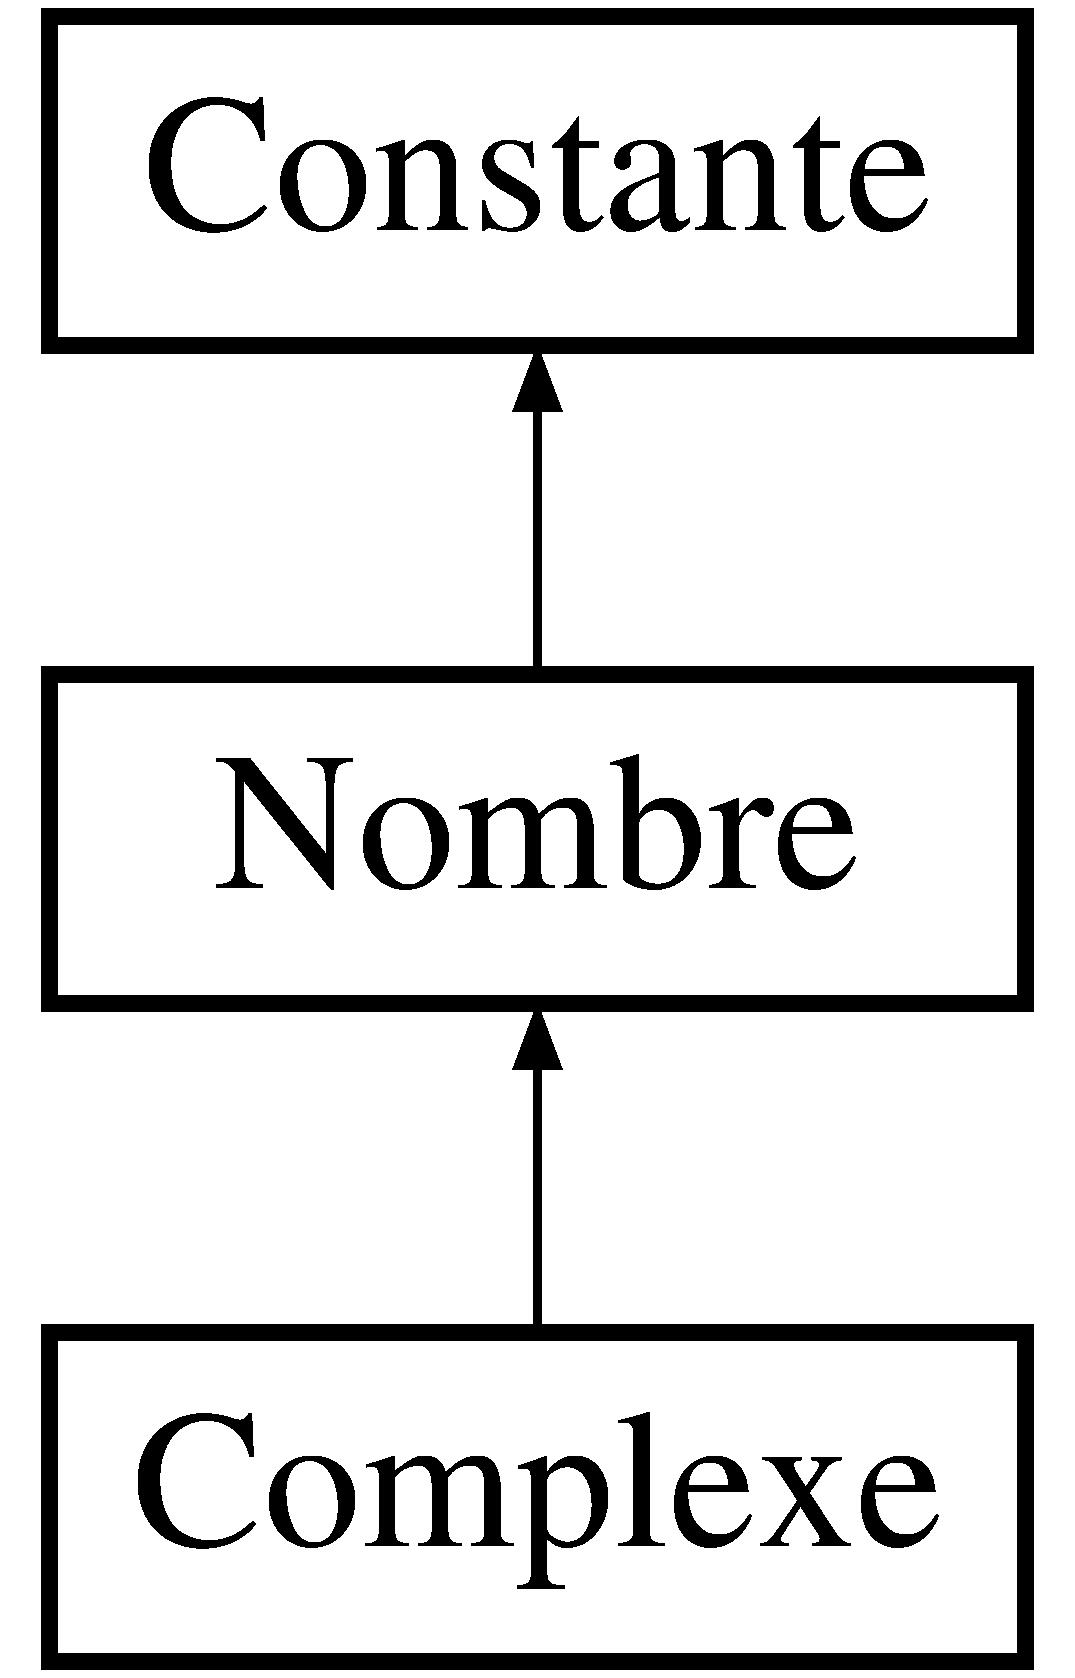
\includegraphics[height=3.000000cm]{classComplexe}
\end{center}
\end{figure}
\subsection*{\-Public \-Member \-Functions}
\begin{DoxyCompactItemize}
\item 
\hyperlink{classComplexe_a562ddecce2f4ab4b7535140fad2d0224}{\-Complexe} (const \hyperlink{classNonComplexe}{\-Non\-Complexe} \&re, const \hyperlink{classNonComplexe}{\-Non\-Complexe} \&im)
\begin{DoxyCompactList}\small\item\em \-Crée un nombre complexe. \end{DoxyCompactList}\item 
\hyperlink{classComplexe_aa0a80cdd5bd70c226641c43c251a0d24}{\-Complexe} (const \hyperlink{classNombre}{\-Nombre} \&re, const \hyperlink{classNombre}{\-Nombre} \&im)
\begin{DoxyCompactList}\small\item\em \-Crée un nombre complexe. \end{DoxyCompactList}\item 
\hyperlink{classComplexe_ac92996231047d39d40e11384bb9311b6}{$\sim$\-Complexe} ()
\item 
\hyperlink{classNombre}{\-Nombre} \& \hyperlink{classComplexe_a699074c8d13ed87b68aeb80463ea1379}{addition} (const \hyperlink{classNombre}{\-Nombre} \&n) const 
\begin{DoxyCompactList}\small\item\em \-Calcule la somme de deux nombres complexe. \-Méthode virtuelle pure héritée et implémentée depuis la classe \hyperlink{classNombre}{\-Nombre}. \end{DoxyCompactList}\item 
\hyperlink{classNombre}{\-Nombre} \& \hyperlink{classComplexe_a54ecc525a7dc0e6491cd3125010b30bf}{soustraction} (const \hyperlink{classNombre}{\-Nombre} \&n) const 
\begin{DoxyCompactList}\small\item\em \-Calcule la soustraction de deux nombres complexe. \-Méthode virtuelle pure héritée et implémentée depuis la classe \hyperlink{classNombre}{\-Nombre}. \end{DoxyCompactList}\item 
\hyperlink{classNombre}{\-Nombre} \& \hyperlink{classComplexe_a1137e6bfa881a8523463adf6f1f15a36}{multiplication} (const \hyperlink{classNombre}{\-Nombre} \&n) const 
\begin{DoxyCompactList}\small\item\em \-Calcule la multiplication de deux nombres complexe. \-Méthode virtuelle pure héritée et implémentée depuis la classe \hyperlink{classNombre}{\-Nombre}. \end{DoxyCompactList}\item 
\hyperlink{classNombre}{\-Nombre} \& \hyperlink{classComplexe_aad8b6ff92139b04c7357a0e566926a20}{division} (const \hyperlink{classNombre}{\-Nombre} \&n) const 
\begin{DoxyCompactList}\small\item\em \-Calcule la division de deux nombres complexe. \-Méthode virtuelle pure héritée et implémentée depuis la classe \hyperlink{classNombre}{\-Nombre}. \end{DoxyCompactList}\item 
\hyperlink{classNombre}{\-Nombre} \& \hyperlink{classComplexe_ae22fa4e15e4d048c6094ae266b6a750e}{sign} () const 
\begin{DoxyCompactList}\small\item\em \-Calcule l'opposée d'un nombre complexe. \-Méthode virtuelle héritée et reimplémentée depuis la classe \hyperlink{classNombre}{\-Nombre}. \end{DoxyCompactList}\item 
\hyperlink{classNombre}{\-Nombre} \& \hyperlink{classComplexe_a4d7ad8bc647f9c3067a0093619f609c0}{sqr} () const 
\begin{DoxyCompactList}\small\item\em \-Calcule le carré d'un nombre complexe. \-Méthode virtuelle héritée et reimplémentée depuis la classe \hyperlink{classNombre}{\-Nombre}. \end{DoxyCompactList}\item 
\hyperlink{classNombre}{\-Nombre} \& \hyperlink{classComplexe_a1f1f8bb3f3c98b55ed934b0c8695bf2f}{cube} () const 
\begin{DoxyCompactList}\small\item\em \-Calcule le cube d'un nombre complexe. \-Méthode virtuelle héritée et reimplémentée depuis la classe \hyperlink{classNombre}{\-Nombre}. \end{DoxyCompactList}\item 
\hyperlink{classNombre}{\-Nombre} \& \hyperlink{classComplexe_a868e620eb3a7cea74b7111254dfd6101}{module} () const 
\begin{DoxyCompactList}\small\item\em \-Calcule le module d'un nombre complexe. \end{DoxyCompactList}\item 
\-Q\-String \hyperlink{classComplexe_a327fd83ec9743fb43c5d47831d8ed45c}{to\-String} () const 
\begin{DoxyCompactList}\small\item\em \-Retourne une chaine de caractères correspondant aux informations encapsulées par un nombre complexe. \-Méthode virtuelle pure héritée et implémentée depuis la classe \hyperlink{classConstante}{\-Constante}. \end{DoxyCompactList}\item 
virtual \hyperlink{classComplexe}{\-Complexe} $\ast$ \hyperlink{classComplexe_a7a7a8d883e959fd7d5f84d5b2b7b2a9e}{clone} () const 
\begin{DoxyCompactList}\small\item\em \-Crée une nouvelle instance de cette classe. \-Méthode virtuelle pure héritée et implémentée depuis la classe \hyperlink{classConstante}{\-Constante}. \end{DoxyCompactList}\end{DoxyCompactItemize}


\subsection{\-Detailed \-Description}
\-Classe permettant de créer et manipuler des constantes de type \hyperlink{classComplexe}{\-Complexe}. \{ hérite de \hyperlink{classNombre}{\-Nombre} \}. 

\subsection{\-Constructor \& \-Destructor \-Documentation}
\hypertarget{classComplexe_a562ddecce2f4ab4b7535140fad2d0224}{\index{\-Complexe@{\-Complexe}!\-Complexe@{\-Complexe}}
\index{\-Complexe@{\-Complexe}!Complexe@{\-Complexe}}
\subsubsection[{\-Complexe}]{\setlength{\rightskip}{0pt plus 5cm}{\bf \-Complexe\-::\-Complexe} (
\begin{DoxyParamCaption}
\item[{const {\bf \-Non\-Complexe} \&}]{re, }
\item[{const {\bf \-Non\-Complexe} \&}]{im}
\end{DoxyParamCaption}
)}}\label{classComplexe_a562ddecce2f4ab4b7535140fad2d0224}


\-Crée un nombre complexe. 


\begin{DoxyParams}{\-Parameters}
{\em re} & \-La partie réelle de ce nombre complexe. \\
\hline
{\em im} & \-La partie imaginaire de ce nombre complexe.\\
\hline
\end{DoxyParams}
\-Crée un nombre complexe. \hypertarget{classComplexe_aa0a80cdd5bd70c226641c43c251a0d24}{\index{\-Complexe@{\-Complexe}!\-Complexe@{\-Complexe}}
\index{\-Complexe@{\-Complexe}!Complexe@{\-Complexe}}
\subsubsection[{\-Complexe}]{\setlength{\rightskip}{0pt plus 5cm}{\bf \-Complexe\-::\-Complexe} (
\begin{DoxyParamCaption}
\item[{const {\bf \-Nombre} \&}]{re, }
\item[{const {\bf \-Nombre} \&}]{im}
\end{DoxyParamCaption}
)}}\label{classComplexe_aa0a80cdd5bd70c226641c43c251a0d24}


\-Crée un nombre complexe. 


\begin{DoxyParams}{\-Parameters}
{\em re} & \-La partie réelle de ce nombre complexe. \\
\hline
{\em im} & \-La partie imaginaire de ce nombre complexe.\\
\hline
\end{DoxyParams}
\-Crée un nombre complexe. \hypertarget{classComplexe_ac92996231047d39d40e11384bb9311b6}{\index{\-Complexe@{\-Complexe}!$\sim$\-Complexe@{$\sim$\-Complexe}}
\index{$\sim$\-Complexe@{$\sim$\-Complexe}!Complexe@{\-Complexe}}
\subsubsection[{$\sim$\-Complexe}]{\setlength{\rightskip}{0pt plus 5cm}{\bf \-Complexe\-::$\sim$\-Complexe} (
\begin{DoxyParamCaption}
{}
\end{DoxyParamCaption}
)}}\label{classComplexe_ac92996231047d39d40e11384bb9311b6}
\-Détruit cette instance de la classe \hyperlink{classComplexe}{\-Complexe}. 

\subsection{\-Member \-Function \-Documentation}
\hypertarget{classComplexe_a699074c8d13ed87b68aeb80463ea1379}{\index{\-Complexe@{\-Complexe}!addition@{addition}}
\index{addition@{addition}!Complexe@{\-Complexe}}
\subsubsection[{addition}]{\setlength{\rightskip}{0pt plus 5cm}{\bf \-Nombre} \& {\bf \-Complexe\-::addition} (
\begin{DoxyParamCaption}
\item[{const {\bf \-Nombre} \&}]{n}
\end{DoxyParamCaption}
) const\hspace{0.3cm}{\ttfamily  \mbox{[}virtual\mbox{]}}}}\label{classComplexe_a699074c8d13ed87b68aeb80463ea1379}


\-Calcule la somme de deux nombres complexe. \-Méthode virtuelle pure héritée et implémentée depuis la classe \hyperlink{classNombre}{\-Nombre}. 


\begin{DoxyParams}{\-Parameters}
{\em n} & \-L'autre nombre complexe. \\
\hline
\end{DoxyParams}
\begin{DoxyReturn}{\-Returns}
\-La somme de deux nombres complexe.
\end{DoxyReturn}
\-Calcule la somme de deux nombres complexe. 

\-Implements \hyperlink{classNombre_ad40df43089fcb34d072b4e955a0eb4fe}{\-Nombre}.

\hypertarget{classComplexe_a7a7a8d883e959fd7d5f84d5b2b7b2a9e}{\index{\-Complexe@{\-Complexe}!clone@{clone}}
\index{clone@{clone}!Complexe@{\-Complexe}}
\subsubsection[{clone}]{\setlength{\rightskip}{0pt plus 5cm}{\bf \-Complexe} $\ast$ {\bf \-Complexe\-::clone} (
\begin{DoxyParamCaption}
{}
\end{DoxyParamCaption}
) const\hspace{0.3cm}{\ttfamily  \mbox{[}inline, virtual\mbox{]}}}}\label{classComplexe_a7a7a8d883e959fd7d5f84d5b2b7b2a9e}


\-Crée une nouvelle instance de cette classe. \-Méthode virtuelle pure héritée et implémentée depuis la classe \hyperlink{classConstante}{\-Constante}. 

\begin{DoxyReturn}{\-Returns}
\-La nouvelle instance de cette classe.
\end{DoxyReturn}
\-Crée une nouvelle instance de cette classe. 

\-Implements \hyperlink{classNombre_afde037df1a7545dbadb537829e90f970}{\-Nombre}.

\hypertarget{classComplexe_a1f1f8bb3f3c98b55ed934b0c8695bf2f}{\index{\-Complexe@{\-Complexe}!cube@{cube}}
\index{cube@{cube}!Complexe@{\-Complexe}}
\subsubsection[{cube}]{\setlength{\rightskip}{0pt plus 5cm}{\bf \-Nombre} \& {\bf \-Complexe\-::cube} (
\begin{DoxyParamCaption}
{}
\end{DoxyParamCaption}
) const\hspace{0.3cm}{\ttfamily  \mbox{[}virtual\mbox{]}}}}\label{classComplexe_a1f1f8bb3f3c98b55ed934b0c8695bf2f}


\-Calcule le cube d'un nombre complexe. \-Méthode virtuelle héritée et reimplémentée depuis la classe \hyperlink{classNombre}{\-Nombre}. 

\begin{DoxyReturn}{\-Returns}
\-Le cube d'un nombre complexe.
\end{DoxyReturn}
\-Calcule le cube d'un nombre complexe. 

\-Reimplemented from \hyperlink{classNombre_a14b257b875fd98a9d53cf275464957e5}{\-Nombre}.

\hypertarget{classComplexe_aad8b6ff92139b04c7357a0e566926a20}{\index{\-Complexe@{\-Complexe}!division@{division}}
\index{division@{division}!Complexe@{\-Complexe}}
\subsubsection[{division}]{\setlength{\rightskip}{0pt plus 5cm}{\bf \-Nombre} \& {\bf \-Complexe\-::division} (
\begin{DoxyParamCaption}
\item[{const {\bf \-Nombre} \&}]{n}
\end{DoxyParamCaption}
) const\hspace{0.3cm}{\ttfamily  \mbox{[}virtual\mbox{]}}}}\label{classComplexe_aad8b6ff92139b04c7357a0e566926a20}


\-Calcule la division de deux nombres complexe. \-Méthode virtuelle pure héritée et implémentée depuis la classe \hyperlink{classNombre}{\-Nombre}. 


\begin{DoxyParams}{\-Parameters}
{\em n} & \-L'autre nombre complexe. \\
\hline
\end{DoxyParams}
\begin{DoxyReturn}{\-Returns}
\-La division de deux nombres complexe.
\end{DoxyReturn}
\-Calcule la division de deux nombres complexe. 

\-Implements \hyperlink{classNombre_ae4e773caee4bb349cdbe7155e26290d6}{\-Nombre}.

\hypertarget{classComplexe_a868e620eb3a7cea74b7111254dfd6101}{\index{\-Complexe@{\-Complexe}!module@{module}}
\index{module@{module}!Complexe@{\-Complexe}}
\subsubsection[{module}]{\setlength{\rightskip}{0pt plus 5cm}{\bf \-Nombre} \& {\bf \-Complexe\-::module} (
\begin{DoxyParamCaption}
{}
\end{DoxyParamCaption}
) const}}\label{classComplexe_a868e620eb3a7cea74b7111254dfd6101}


\-Calcule le module d'un nombre complexe. 

\begin{DoxyReturn}{\-Returns}
\-Le module d'un nombre complexe.
\end{DoxyReturn}
\-Calcule le module d'un nombre complexe. \hypertarget{classComplexe_a1137e6bfa881a8523463adf6f1f15a36}{\index{\-Complexe@{\-Complexe}!multiplication@{multiplication}}
\index{multiplication@{multiplication}!Complexe@{\-Complexe}}
\subsubsection[{multiplication}]{\setlength{\rightskip}{0pt plus 5cm}{\bf \-Nombre} \& {\bf \-Complexe\-::multiplication} (
\begin{DoxyParamCaption}
\item[{const {\bf \-Nombre} \&}]{n}
\end{DoxyParamCaption}
) const\hspace{0.3cm}{\ttfamily  \mbox{[}virtual\mbox{]}}}}\label{classComplexe_a1137e6bfa881a8523463adf6f1f15a36}


\-Calcule la multiplication de deux nombres complexe. \-Méthode virtuelle pure héritée et implémentée depuis la classe \hyperlink{classNombre}{\-Nombre}. 


\begin{DoxyParams}{\-Parameters}
{\em n} & \-L'autre nombre complexe. \\
\hline
\end{DoxyParams}
\begin{DoxyReturn}{\-Returns}
\-La multiplication de deux nombres complexe.
\end{DoxyReturn}
\-Calcule la multiplication de deux nombres complexe. 

\-Implements \hyperlink{classNombre_a742022c5e875fe24046d1c28cf043b42}{\-Nombre}.

\hypertarget{classComplexe_ae22fa4e15e4d048c6094ae266b6a750e}{\index{\-Complexe@{\-Complexe}!sign@{sign}}
\index{sign@{sign}!Complexe@{\-Complexe}}
\subsubsection[{sign}]{\setlength{\rightskip}{0pt plus 5cm}{\bf \-Nombre} \& {\bf \-Complexe\-::sign} (
\begin{DoxyParamCaption}
{}
\end{DoxyParamCaption}
) const\hspace{0.3cm}{\ttfamily  \mbox{[}virtual\mbox{]}}}}\label{classComplexe_ae22fa4e15e4d048c6094ae266b6a750e}


\-Calcule l'opposée d'un nombre complexe. \-Méthode virtuelle héritée et reimplémentée depuis la classe \hyperlink{classNombre}{\-Nombre}. 

\begin{DoxyReturn}{\-Returns}
\-L'opposée d'un nombre complexe.
\end{DoxyReturn}
\-Calcule l'opposée d'un nombre complexe. 

\-Reimplemented from \hyperlink{classNombre_a3fb106bcd953c9d3e03609bf1d49f2e7}{\-Nombre}.

\hypertarget{classComplexe_a54ecc525a7dc0e6491cd3125010b30bf}{\index{\-Complexe@{\-Complexe}!soustraction@{soustraction}}
\index{soustraction@{soustraction}!Complexe@{\-Complexe}}
\subsubsection[{soustraction}]{\setlength{\rightskip}{0pt plus 5cm}{\bf \-Nombre} \& {\bf \-Complexe\-::soustraction} (
\begin{DoxyParamCaption}
\item[{const {\bf \-Nombre} \&}]{n}
\end{DoxyParamCaption}
) const\hspace{0.3cm}{\ttfamily  \mbox{[}virtual\mbox{]}}}}\label{classComplexe_a54ecc525a7dc0e6491cd3125010b30bf}


\-Calcule la soustraction de deux nombres complexe. \-Méthode virtuelle pure héritée et implémentée depuis la classe \hyperlink{classNombre}{\-Nombre}. 


\begin{DoxyParams}{\-Parameters}
{\em n} & \-L'autre nombre complexe. \\
\hline
\end{DoxyParams}
\begin{DoxyReturn}{\-Returns}
\-La soustraction de deux nombres complexe.
\end{DoxyReturn}
\-Calcule la soustraction de deux nombres complexe. 

\-Implements \hyperlink{classNombre_aae525a90cd3ddeda1ce8349a23634e75}{\-Nombre}.

\hypertarget{classComplexe_a4d7ad8bc647f9c3067a0093619f609c0}{\index{\-Complexe@{\-Complexe}!sqr@{sqr}}
\index{sqr@{sqr}!Complexe@{\-Complexe}}
\subsubsection[{sqr}]{\setlength{\rightskip}{0pt plus 5cm}{\bf \-Nombre} \& {\bf \-Complexe\-::sqr} (
\begin{DoxyParamCaption}
{}
\end{DoxyParamCaption}
) const\hspace{0.3cm}{\ttfamily  \mbox{[}virtual\mbox{]}}}}\label{classComplexe_a4d7ad8bc647f9c3067a0093619f609c0}


\-Calcule le carré d'un nombre complexe. \-Méthode virtuelle héritée et reimplémentée depuis la classe \hyperlink{classNombre}{\-Nombre}. 

\begin{DoxyReturn}{\-Returns}
\-Le carré d'un nombre complexe.
\end{DoxyReturn}
\-Calcule le carré d'un nombre complexe. 

\-Reimplemented from \hyperlink{classNombre_a43b5ad781c1274196907939a36ecefcf}{\-Nombre}.

\hypertarget{classComplexe_a327fd83ec9743fb43c5d47831d8ed45c}{\index{\-Complexe@{\-Complexe}!to\-String@{to\-String}}
\index{to\-String@{to\-String}!Complexe@{\-Complexe}}
\subsubsection[{to\-String}]{\setlength{\rightskip}{0pt plus 5cm}\-Q\-String {\bf \-Complexe\-::to\-String} (
\begin{DoxyParamCaption}
{}
\end{DoxyParamCaption}
) const\hspace{0.3cm}{\ttfamily  \mbox{[}virtual\mbox{]}}}}\label{classComplexe_a327fd83ec9743fb43c5d47831d8ed45c}


\-Retourne une chaine de caractères correspondant aux informations encapsulées par un nombre complexe. \-Méthode virtuelle pure héritée et implémentée depuis la classe \hyperlink{classConstante}{\-Constante}. 

\begin{DoxyReturn}{\-Returns}
\-Une chaine de caractères correspondant aux informations encapsulées par un nombre complexe.
\end{DoxyReturn}
\-Retourne une chaine de caractères correspondant aux informations encapsulées par un nombre complexe. 

\-Implements \hyperlink{classNombre_a8df232159bfd0e9f7e153cc73c8b128c}{\-Nombre}.



\-The documentation for this class was generated from the following files\-:\begin{DoxyCompactItemize}
\item 
\hyperlink{Complexe_8h}{\-Complexe.\-h}\item 
\-Complexe.\-cpp\end{DoxyCompactItemize}

\hypertarget{classConstante}{\section{\-Constante \-Class \-Reference}
\label{classConstante}\index{\-Constante@{\-Constante}}
}


\-Classe abstraite étant utilisée comme interface pour les classes qui en héritent.  




{\ttfamily \#include $<$\-Constante.\-h$>$}

\-Inheritance diagram for \-Constante\-:\begin{figure}[H]
\begin{center}
\leavevmode
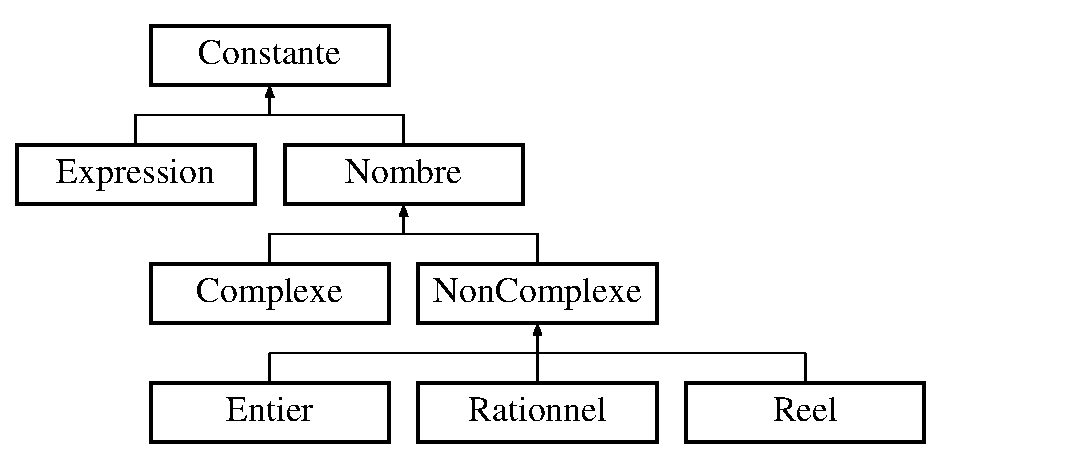
\includegraphics[height=4.000000cm]{classConstante}
\end{center}
\end{figure}
\subsection*{\-Public \-Member \-Functions}
\begin{DoxyCompactItemize}
\item 
void \hyperlink{classConstante_aa1c1c46c040775cbbdf5bee0bba452f9}{afficher} () const 
\item 
virtual \hyperlink{classConstante}{\-Constante} $\ast$ \hyperlink{classConstante_a5769ea385161e02bd2d1bcadefc2c510}{clone} () const =0
\begin{DoxyCompactList}\small\item\em \-Crée une nouvelle instance de cette classe. \-Méthode virtuelle pure. \end{DoxyCompactList}\item 
virtual \-Q\-String \hyperlink{classConstante_ad5ea6850196ee9f86b74c74009a87ab1}{to\-String} () const =0
\begin{DoxyCompactList}\small\item\em \-Retourne une chaine de caractères correspondant aux informations encapsulées par une constante. \-Méthode virtuelle pure. \end{DoxyCompactList}\end{DoxyCompactItemize}


\subsection{\-Detailed \-Description}
\-Classe abstraite étant utilisée comme interface pour les classes qui en héritent. 

\-Le \-Design \-Pattern \-Template \-Method est utilisé. 

\subsection{\-Member \-Function \-Documentation}
\hypertarget{classConstante_aa1c1c46c040775cbbdf5bee0bba452f9}{\index{\-Constante@{\-Constante}!afficher@{afficher}}
\index{afficher@{afficher}!Constante@{\-Constante}}
\subsubsection[{afficher}]{\setlength{\rightskip}{0pt plus 5cm}void {\bf \-Constante\-::afficher} (
\begin{DoxyParamCaption}
{}
\end{DoxyParamCaption}
) const}}\label{classConstante_aa1c1c46c040775cbbdf5bee0bba452f9}
\-Affiche les informations encapsulées par un nombre complexe. \hypertarget{classConstante_a5769ea385161e02bd2d1bcadefc2c510}{\index{\-Constante@{\-Constante}!clone@{clone}}
\index{clone@{clone}!Constante@{\-Constante}}
\subsubsection[{clone}]{\setlength{\rightskip}{0pt plus 5cm}virtual {\bf \-Constante}$\ast$ {\bf \-Constante\-::clone} (
\begin{DoxyParamCaption}
{}
\end{DoxyParamCaption}
) const\hspace{0.3cm}{\ttfamily  \mbox{[}pure virtual\mbox{]}}}}\label{classConstante_a5769ea385161e02bd2d1bcadefc2c510}


\-Crée une nouvelle instance de cette classe. \-Méthode virtuelle pure. 

\begin{DoxyReturn}{\-Returns}
\-La nouvelle instance de cette classe.
\end{DoxyReturn}
\-Crée une nouvelle instance de cette classe. 

\-Implemented in \hyperlink{classNonComplexe_a7f1a3881b59680f3d3a7809c75ab2138}{\-Non\-Complexe}, \hyperlink{classRationnel_a422ec3e0c4465d08c4e9deceda6c442c}{\-Rationnel}, \hyperlink{classComplexe_a7a7a8d883e959fd7d5f84d5b2b7b2a9e}{\-Complexe}, \hyperlink{classEntier_aca1eef6372c8d74274bffd435888ef57}{\-Entier}, \hyperlink{classNombre_afde037df1a7545dbadb537829e90f970}{\-Nombre}, \hyperlink{classReel_ab53c7d10a93c702bd7ccde897fc396df}{\-Reel}, and \hyperlink{classExpression_ad357e8bb1174b3582833ebcbf6d6e232}{\-Expression}.

\hypertarget{classConstante_ad5ea6850196ee9f86b74c74009a87ab1}{\index{\-Constante@{\-Constante}!to\-String@{to\-String}}
\index{to\-String@{to\-String}!Constante@{\-Constante}}
\subsubsection[{to\-String}]{\setlength{\rightskip}{0pt plus 5cm}virtual \-Q\-String {\bf \-Constante\-::to\-String} (
\begin{DoxyParamCaption}
{}
\end{DoxyParamCaption}
) const\hspace{0.3cm}{\ttfamily  \mbox{[}pure virtual\mbox{]}}}}\label{classConstante_ad5ea6850196ee9f86b74c74009a87ab1}


\-Retourne une chaine de caractères correspondant aux informations encapsulées par une constante. \-Méthode virtuelle pure. 

\begin{DoxyReturn}{\-Returns}
\-Une chaine de caractères correspondant aux informations encapsulées par une constante.
\end{DoxyReturn}
\-Retourne une chaine de caractères correspondant aux informations encapsulées par une constante. 

\-Implemented in \hyperlink{classNonComplexe_abae1947a8f9f582f94d5e791ce4624d6}{\-Non\-Complexe}, \hyperlink{classRationnel_a41bc89d21ce161818f67ccfe296766c0}{\-Rationnel}, \hyperlink{classEntier_aa960356dfeae8af6dfa2cd25136a1a6f}{\-Entier}, \hyperlink{classNombre_a8df232159bfd0e9f7e153cc73c8b128c}{\-Nombre}, \hyperlink{classReel_a990e8324822ba3dbc64fc7ff727411e2}{\-Reel}, \hyperlink{classComplexe_a327fd83ec9743fb43c5d47831d8ed45c}{\-Complexe}, and \hyperlink{classExpression_a60e6e305cdd8e878df2e3081ae15a4d0}{\-Expression}.



\-The documentation for this class was generated from the following files\-:\begin{DoxyCompactItemize}
\item 
\hyperlink{Constante_8h}{\-Constante.\-h}\item 
\-Constante.\-cpp\end{DoxyCompactItemize}

\hypertarget{classDialog}{\section{\-Dialog \-Class \-Reference}
\label{classDialog}\index{\-Dialog@{\-Dialog}}
}
\subsection*{\-Public \-Member \-Functions}
\begin{DoxyCompactItemize}
\item 
\hypertarget{classDialog_acfa2063f9f962d394c6a645b6e7e08d8}{{\bfseries \-Dialog} (\-Q\-Widget $\ast$parent=0)}\label{classDialog_acfa2063f9f962d394c6a645b6e7e08d8}

\end{DoxyCompactItemize}
\subsection*{\-Public \-Attributes}
\begin{DoxyCompactItemize}
\item 
\hypertarget{classDialog_aaa4b5bfb9a0f64900d524f14bc32e6df}{\-Ui\-::\-Dialog $\ast$ {\bfseries ui}}\label{classDialog_aaa4b5bfb9a0f64900d524f14bc32e6df}

\end{DoxyCompactItemize}


\-The documentation for this class was generated from the following files\-:\begin{DoxyCompactItemize}
\item 
\hyperlink{dialog_8h}{dialog.\-h}\item 
dialog.\-cpp\end{DoxyCompactItemize}

\hypertarget{classEntier}{\section{\-Entier \-Class \-Reference}
\label{classEntier}\index{\-Entier@{\-Entier}}
}


\-Classe permettant de créer et manipuler des constantes de type \hyperlink{classEntier}{\-Entier}. \{ hérite de \hyperlink{classNonComplexe}{\-Non\-Complexe} \}.  




{\ttfamily \#include $<$\-Entier.\-h$>$}

\-Inheritance diagram for \-Entier\-:\begin{figure}[H]
\begin{center}
\leavevmode
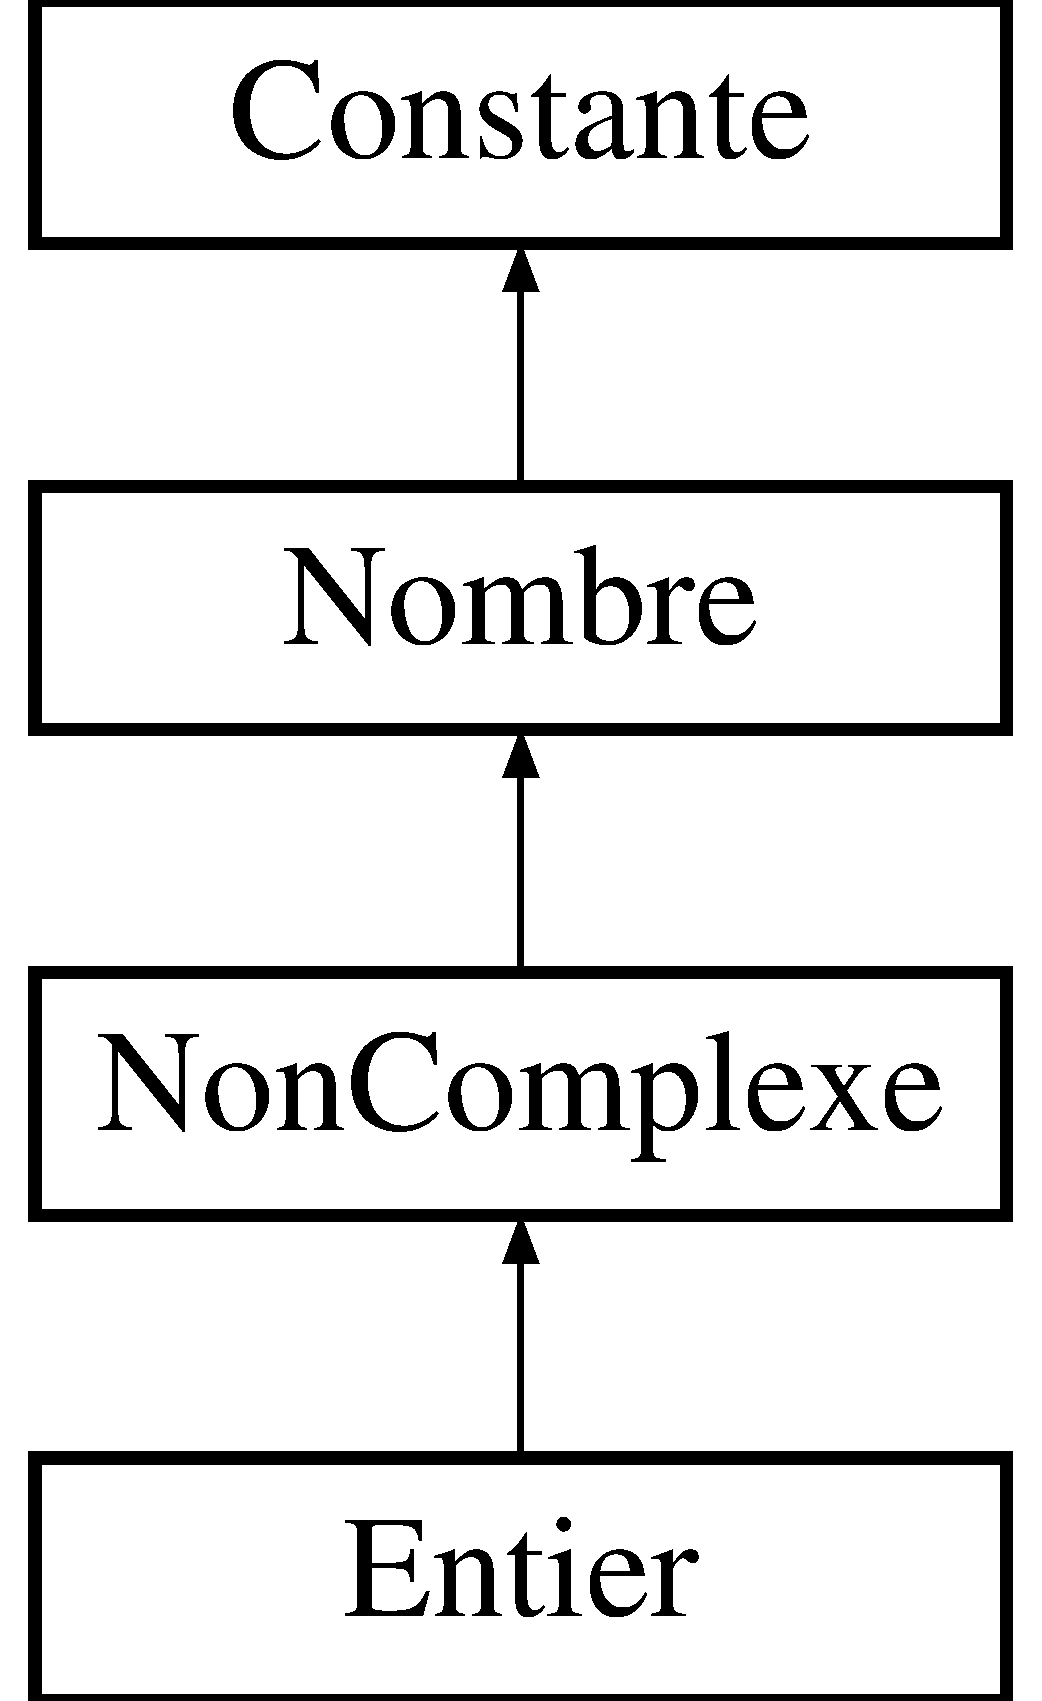
\includegraphics[height=4.000000cm]{classEntier}
\end{center}
\end{figure}
\subsection*{\-Public \-Member \-Functions}
\begin{DoxyCompactItemize}
\item 
\hyperlink{classEntier_a8eea484d9052df02d4ac9e03019863ec}{\-Entier} (int x=0)
\begin{DoxyCompactList}\small\item\em \-Crée un nombre entier. \end{DoxyCompactList}\item 
\hyperlink{classNombre}{\-Nombre} \& \hyperlink{classEntier_abbb59e17a481b81158182411a46faf82}{addition} (const \hyperlink{classNombre}{\-Nombre} \&n) const 
\begin{DoxyCompactList}\small\item\em \-Calcule la somme de ce nombre entier et d'un nombre. \-Méthode virtuelle pure héritée et implémentée depuis la classe \hyperlink{classNombre}{\-Nombre}. \end{DoxyCompactList}\item 
\hyperlink{classNombre}{\-Nombre} \& \hyperlink{classEntier_aad2b72821451bf5a0445f1cccc8ab1cb}{soustraction} (const \hyperlink{classNombre}{\-Nombre} \&n) const 
\begin{DoxyCompactList}\small\item\em \-Calcule la soustraction de ce nombre entier et d'un nombre. \-Méthode virtuelle pure héritée et implémentée depuis la classe \hyperlink{classNombre}{\-Nombre}. \end{DoxyCompactList}\item 
\hyperlink{classNombre}{\-Nombre} \& \hyperlink{classEntier_a4e51200ae8e5e704ecb349d2d69f0dbf}{multiplication} (const \hyperlink{classNombre}{\-Nombre} \&n) const 
\begin{DoxyCompactList}\small\item\em \-Calcule la multiplication de ce nombre entier et d'un nombre. \-Méthode virtuelle pure héritée et implémentée depuis la classe \hyperlink{classNombre}{\-Nombre}. \end{DoxyCompactList}\item 
\hyperlink{classNombre}{\-Nombre} \& \hyperlink{classEntier_a968f1bd92ad6fc703aa3160921d905f7}{division} (const \hyperlink{classNombre}{\-Nombre} \&n) const 
\begin{DoxyCompactList}\small\item\em \-Calcule la division de ce nombre entier et d'un nombre. \-Méthode virtuelle pure héritée et implémentée depuis la classe \hyperlink{classNombre}{\-Nombre}. \end{DoxyCompactList}\item 
\hyperlink{classNonComplexe}{\-Non\-Complexe} \& \hyperlink{classEntier_a0d34eb382eb7329b16552d191592ed27}{to\-Entier} () const 
\begin{DoxyCompactList}\small\item\em \-Converti le nombre entier en un nombre entier. \-Méthode virtuelle pure héritée et implémentée depuis la classe \hyperlink{classNonComplexe}{\-Non\-Complexe}. \end{DoxyCompactList}\item 
\hyperlink{classNonComplexe}{\-Non\-Complexe} \& \hyperlink{classEntier_a8ac645f157658a958ec4b46f9f60d3cd}{to\-Reel} () const 
\begin{DoxyCompactList}\small\item\em \-Converti le nombre entier en un nombre réel. \-Méthode virtuelle pure héritée et implémentée depuis la classe \hyperlink{classNonComplexe}{\-Non\-Complexe}. \end{DoxyCompactList}\item 
\hyperlink{classNonComplexe}{\-Non\-Complexe} \& \hyperlink{classEntier_a7a7e540ab2ea666819e6f916ed6617de}{to\-Rationnel} () const 
\begin{DoxyCompactList}\small\item\em \-Converti le nombre entier en un nombre rationnel. \-Méthode virtuelle pure héritée et implémentée depuis la classe \hyperlink{classNonComplexe}{\-Non\-Complexe}. \end{DoxyCompactList}\item 
\hyperlink{classNonComplexe}{\-Non\-Complexe} \& \hyperlink{classEntier_a33148f1d942abe9f810542ae8b71e653}{to\-Complexe} () const 
\begin{DoxyCompactList}\small\item\em \-Converti le nombre entier en un nombre complexe. \-Méthode virtuelle pure héritée et implémentée depuis la classe \hyperlink{classNonComplexe}{\-Non\-Complexe}. \end{DoxyCompactList}\item 
\hyperlink{classEntier}{\-Entier} \& \hyperlink{classEntier_a79059e2d7c89d2e27a6fba79efb392d1}{mod} (const \hyperlink{classEntier}{\-Entier} \&e)
\begin{DoxyCompactList}\small\item\em \-Calcule le module de ce nombre entier. \end{DoxyCompactList}\item 
\hyperlink{classEntier}{\-Entier} \& \hyperlink{classEntier_af330a9378ef16e9e5381bf0d0a97d443}{fact} ()
\begin{DoxyCompactList}\small\item\em \-Calcule la factorielle de ce nombre entier. \end{DoxyCompactList}\item 
int \hyperlink{classEntier_ae9b5afc145e621aba2b872c9dcd4b3ba}{get\-X} () const 
\begin{DoxyCompactList}\small\item\em \-Retourne l'entier de ce nombre entier. \end{DoxyCompactList}\item 
virtual \hyperlink{classEntier}{\-Entier} $\ast$ \hyperlink{classEntier_aca1eef6372c8d74274bffd435888ef57}{clone} () const 
\begin{DoxyCompactList}\small\item\em \-Crée une nouvelle instance de cette classe. \-Méthode virtuelle pure héritée et implémentée depuis la classe \hyperlink{classConstante}{\-Constante}. \end{DoxyCompactList}\item 
\-Q\-String \hyperlink{classEntier_aa960356dfeae8af6dfa2cd25136a1a6f}{to\-String} () const 
\begin{DoxyCompactList}\small\item\em \-Retourne une chaine de caractères correspondant aux informations encapsulées par un nombre entier. \-Méthode virtuelle pure héritée et implémentée depuis la classe \hyperlink{classConstante}{\-Constante}. \end{DoxyCompactList}\end{DoxyCompactItemize}


\subsection{\-Detailed \-Description}
\-Classe permettant de créer et manipuler des constantes de type \hyperlink{classEntier}{\-Entier}. \{ hérite de \hyperlink{classNonComplexe}{\-Non\-Complexe} \}. 

\subsection{\-Constructor \& \-Destructor \-Documentation}
\hypertarget{classEntier_a8eea484d9052df02d4ac9e03019863ec}{\index{\-Entier@{\-Entier}!\-Entier@{\-Entier}}
\index{\-Entier@{\-Entier}!Entier@{\-Entier}}
\subsubsection[{\-Entier}]{\setlength{\rightskip}{0pt plus 5cm}{\bf \-Entier\-::\-Entier} (
\begin{DoxyParamCaption}
\item[{int}]{x = {\ttfamily 0}}
\end{DoxyParamCaption}
)\hspace{0.3cm}{\ttfamily  \mbox{[}inline\mbox{]}}}}\label{classEntier_a8eea484d9052df02d4ac9e03019863ec}


\-Crée un nombre entier. 


\begin{DoxyParams}{\-Parameters}
{\em x} & \-La valeur de ce nombre entier.\\
\hline
\end{DoxyParams}
\-Crée un nombre entier de valeur donnée. 

\subsection{\-Member \-Function \-Documentation}
\hypertarget{classEntier_abbb59e17a481b81158182411a46faf82}{\index{\-Entier@{\-Entier}!addition@{addition}}
\index{addition@{addition}!Entier@{\-Entier}}
\subsubsection[{addition}]{\setlength{\rightskip}{0pt plus 5cm}{\bf \-Nombre} \& {\bf \-Entier\-::addition} (
\begin{DoxyParamCaption}
\item[{const {\bf \-Nombre} \&}]{n}
\end{DoxyParamCaption}
) const\hspace{0.3cm}{\ttfamily  \mbox{[}virtual\mbox{]}}}}\label{classEntier_abbb59e17a481b81158182411a46faf82}


\-Calcule la somme de ce nombre entier et d'un nombre. \-Méthode virtuelle pure héritée et implémentée depuis la classe \hyperlink{classNombre}{\-Nombre}. 


\begin{DoxyParams}{\-Parameters}
{\em n} & \-Un nombre. \\
\hline
\end{DoxyParams}
\begin{DoxyReturn}{\-Returns}
\-La somme de ce nombre entier et d'un nombre.
\end{DoxyReturn}
\-Calcule la somme de ce nombre entier et d'un nombre. 

\-Implements \hyperlink{classNonComplexe_a1ed6f047d5c576f03616535e3e92ab39}{\-Non\-Complexe}.

\hypertarget{classEntier_aca1eef6372c8d74274bffd435888ef57}{\index{\-Entier@{\-Entier}!clone@{clone}}
\index{clone@{clone}!Entier@{\-Entier}}
\subsubsection[{clone}]{\setlength{\rightskip}{0pt plus 5cm}{\bf \-Entier} $\ast$ {\bf \-Entier\-::clone} (
\begin{DoxyParamCaption}
{}
\end{DoxyParamCaption}
) const\hspace{0.3cm}{\ttfamily  \mbox{[}inline, virtual\mbox{]}}}}\label{classEntier_aca1eef6372c8d74274bffd435888ef57}


\-Crée une nouvelle instance de cette classe. \-Méthode virtuelle pure héritée et implémentée depuis la classe \hyperlink{classConstante}{\-Constante}. 

\begin{DoxyReturn}{\-Returns}
\-La nouvelle instance de cette classe.
\end{DoxyReturn}
\-Crée une nouvelle instance de cette classe. 

\-Implements \hyperlink{classNonComplexe_a7f1a3881b59680f3d3a7809c75ab2138}{\-Non\-Complexe}.

\hypertarget{classEntier_a968f1bd92ad6fc703aa3160921d905f7}{\index{\-Entier@{\-Entier}!division@{division}}
\index{division@{division}!Entier@{\-Entier}}
\subsubsection[{division}]{\setlength{\rightskip}{0pt plus 5cm}{\bf \-Nombre} \& {\bf \-Entier\-::division} (
\begin{DoxyParamCaption}
\item[{const {\bf \-Nombre} \&}]{n}
\end{DoxyParamCaption}
) const\hspace{0.3cm}{\ttfamily  \mbox{[}virtual\mbox{]}}}}\label{classEntier_a968f1bd92ad6fc703aa3160921d905f7}


\-Calcule la division de ce nombre entier et d'un nombre. \-Méthode virtuelle pure héritée et implémentée depuis la classe \hyperlink{classNombre}{\-Nombre}. 


\begin{DoxyParams}{\-Parameters}
{\em n} & \-Un nombre. \\
\hline
\end{DoxyParams}
\begin{DoxyReturn}{\-Returns}
\-La division de ce nombre entier et d'un nombre.
\end{DoxyReturn}
\-Calcule la division de ce nombre entier et d'un nombre. 

\-Implements \hyperlink{classNonComplexe_a1af698f4c7d50e69f2c7dfa3e7998cdd}{\-Non\-Complexe}.

\hypertarget{classEntier_af330a9378ef16e9e5381bf0d0a97d443}{\index{\-Entier@{\-Entier}!fact@{fact}}
\index{fact@{fact}!Entier@{\-Entier}}
\subsubsection[{fact}]{\setlength{\rightskip}{0pt plus 5cm}{\bf \-Entier} \& {\bf \-Entier\-::fact} (
\begin{DoxyParamCaption}
{}
\end{DoxyParamCaption}
)}}\label{classEntier_af330a9378ef16e9e5381bf0d0a97d443}


\-Calcule la factorielle de ce nombre entier. 

\begin{DoxyReturn}{\-Returns}
\-Une référence vers la factorielle de ce nombre entier.
\end{DoxyReturn}
\-Calcule la factorielle de ce nombre entier. \hypertarget{classEntier_ae9b5afc145e621aba2b872c9dcd4b3ba}{\index{\-Entier@{\-Entier}!get\-X@{get\-X}}
\index{get\-X@{get\-X}!Entier@{\-Entier}}
\subsubsection[{get\-X}]{\setlength{\rightskip}{0pt plus 5cm}int {\bf \-Entier\-::get\-X} (
\begin{DoxyParamCaption}
{}
\end{DoxyParamCaption}
) const\hspace{0.3cm}{\ttfamily  \mbox{[}inline\mbox{]}}}}\label{classEntier_ae9b5afc145e621aba2b872c9dcd4b3ba}


\-Retourne l'entier de ce nombre entier. 

\begin{DoxyReturn}{\-Returns}
\-Un entier.
\end{DoxyReturn}
\-Retourne l'entier de ce nombre entier. \hypertarget{classEntier_a79059e2d7c89d2e27a6fba79efb392d1}{\index{\-Entier@{\-Entier}!mod@{mod}}
\index{mod@{mod}!Entier@{\-Entier}}
\subsubsection[{mod}]{\setlength{\rightskip}{0pt plus 5cm}{\bf \-Entier} \& {\bf \-Entier\-::mod} (
\begin{DoxyParamCaption}
\item[{const {\bf \-Entier} \&}]{e}
\end{DoxyParamCaption}
)}}\label{classEntier_a79059e2d7c89d2e27a6fba79efb392d1}


\-Calcule le module de ce nombre entier. 


\begin{DoxyParams}{\-Parameters}
{\em \-Une} & référence constante vers un nombre entier correspondant au diviseur. \\
\hline
\end{DoxyParams}
\begin{DoxyReturn}{\-Returns}
\-Une référence vers le modulo de ce nombre entier.
\end{DoxyReturn}
\-Calcule le module de ce nombre entier. \hypertarget{classEntier_a4e51200ae8e5e704ecb349d2d69f0dbf}{\index{\-Entier@{\-Entier}!multiplication@{multiplication}}
\index{multiplication@{multiplication}!Entier@{\-Entier}}
\subsubsection[{multiplication}]{\setlength{\rightskip}{0pt plus 5cm}{\bf \-Nombre} \& {\bf \-Entier\-::multiplication} (
\begin{DoxyParamCaption}
\item[{const {\bf \-Nombre} \&}]{n}
\end{DoxyParamCaption}
) const\hspace{0.3cm}{\ttfamily  \mbox{[}virtual\mbox{]}}}}\label{classEntier_a4e51200ae8e5e704ecb349d2d69f0dbf}


\-Calcule la multiplication de ce nombre entier et d'un nombre. \-Méthode virtuelle pure héritée et implémentée depuis la classe \hyperlink{classNombre}{\-Nombre}. 


\begin{DoxyParams}{\-Parameters}
{\em n} & \-Un nombre. \\
\hline
\end{DoxyParams}
\begin{DoxyReturn}{\-Returns}
\-La multiplication de ce nombre entier et d'un nombre.
\end{DoxyReturn}
\-Calcule la multiplication de ce nombre entier et d'un nombre. 

\-Implements \hyperlink{classNonComplexe_a7343c4742a895813a4b031fb67170dc8}{\-Non\-Complexe}.

\hypertarget{classEntier_aad2b72821451bf5a0445f1cccc8ab1cb}{\index{\-Entier@{\-Entier}!soustraction@{soustraction}}
\index{soustraction@{soustraction}!Entier@{\-Entier}}
\subsubsection[{soustraction}]{\setlength{\rightskip}{0pt plus 5cm}{\bf \-Nombre} \& {\bf \-Entier\-::soustraction} (
\begin{DoxyParamCaption}
\item[{const {\bf \-Nombre} \&}]{n}
\end{DoxyParamCaption}
) const\hspace{0.3cm}{\ttfamily  \mbox{[}virtual\mbox{]}}}}\label{classEntier_aad2b72821451bf5a0445f1cccc8ab1cb}


\-Calcule la soustraction de ce nombre entier et d'un nombre. \-Méthode virtuelle pure héritée et implémentée depuis la classe \hyperlink{classNombre}{\-Nombre}. 


\begin{DoxyParams}{\-Parameters}
{\em n} & \-Un nombre. \\
\hline
\end{DoxyParams}
\begin{DoxyReturn}{\-Returns}
\-La soustraction de ce nombre entier et d'un nombre.
\end{DoxyReturn}
\-Calcule la soustraction de ce nombre entier et d'un nombre. 

\-Implements \hyperlink{classNonComplexe_ac7e41f7e2f5422687985a5fe501e243f}{\-Non\-Complexe}.

\hypertarget{classEntier_a33148f1d942abe9f810542ae8b71e653}{\index{\-Entier@{\-Entier}!to\-Complexe@{to\-Complexe}}
\index{to\-Complexe@{to\-Complexe}!Entier@{\-Entier}}
\subsubsection[{to\-Complexe}]{\setlength{\rightskip}{0pt plus 5cm}{\bf \-Non\-Complexe} \& {\bf \-Entier\-::to\-Complexe} (
\begin{DoxyParamCaption}
{}
\end{DoxyParamCaption}
) const\hspace{0.3cm}{\ttfamily  \mbox{[}virtual\mbox{]}}}}\label{classEntier_a33148f1d942abe9f810542ae8b71e653}


\-Converti le nombre entier en un nombre complexe. \-Méthode virtuelle pure héritée et implémentée depuis la classe \hyperlink{classNonComplexe}{\-Non\-Complexe}. 

\begin{DoxyReturn}{\-Returns}
\-Une référence vers un nombre non complexe emmagasinant en réalité un nombre complexe.
\end{DoxyReturn}
\-Converti le nombre entier en un nombre complexe. 

\-Implements \hyperlink{classNonComplexe_ad29a8407072d909cd204945d5cd5bc17}{\-Non\-Complexe}.

\hypertarget{classEntier_a0d34eb382eb7329b16552d191592ed27}{\index{\-Entier@{\-Entier}!to\-Entier@{to\-Entier}}
\index{to\-Entier@{to\-Entier}!Entier@{\-Entier}}
\subsubsection[{to\-Entier}]{\setlength{\rightskip}{0pt plus 5cm}{\bf \-Non\-Complexe} \& {\bf \-Entier\-::to\-Entier} (
\begin{DoxyParamCaption}
{}
\end{DoxyParamCaption}
) const\hspace{0.3cm}{\ttfamily  \mbox{[}virtual\mbox{]}}}}\label{classEntier_a0d34eb382eb7329b16552d191592ed27}


\-Converti le nombre entier en un nombre entier. \-Méthode virtuelle pure héritée et implémentée depuis la classe \hyperlink{classNonComplexe}{\-Non\-Complexe}. 

\begin{DoxyReturn}{\-Returns}
\-Une référence vers un nombre non complexe emmagasinant en réalité un nombre entier.
\end{DoxyReturn}
\-Converti le nombre entier en un nombre entier. 

\-Implements \hyperlink{classNonComplexe_af5751554285a6bf0bb1433a059bbfcdd}{\-Non\-Complexe}.

\hypertarget{classEntier_a7a7e540ab2ea666819e6f916ed6617de}{\index{\-Entier@{\-Entier}!to\-Rationnel@{to\-Rationnel}}
\index{to\-Rationnel@{to\-Rationnel}!Entier@{\-Entier}}
\subsubsection[{to\-Rationnel}]{\setlength{\rightskip}{0pt plus 5cm}{\bf \-Non\-Complexe} \& {\bf \-Entier\-::to\-Rationnel} (
\begin{DoxyParamCaption}
{}
\end{DoxyParamCaption}
) const\hspace{0.3cm}{\ttfamily  \mbox{[}virtual\mbox{]}}}}\label{classEntier_a7a7e540ab2ea666819e6f916ed6617de}


\-Converti le nombre entier en un nombre rationnel. \-Méthode virtuelle pure héritée et implémentée depuis la classe \hyperlink{classNonComplexe}{\-Non\-Complexe}. 

\begin{DoxyReturn}{\-Returns}
\-Une référence vers un nombre non complexe emmagasinant en réalité un nombre rationnel.
\end{DoxyReturn}
\-Converti le nombre entier en un nombre rationnel. 

\-Implements \hyperlink{classNonComplexe_a5c416e7c9d4c011c67b69b112cc30cc1}{\-Non\-Complexe}.

\hypertarget{classEntier_a8ac645f157658a958ec4b46f9f60d3cd}{\index{\-Entier@{\-Entier}!to\-Reel@{to\-Reel}}
\index{to\-Reel@{to\-Reel}!Entier@{\-Entier}}
\subsubsection[{to\-Reel}]{\setlength{\rightskip}{0pt plus 5cm}{\bf \-Non\-Complexe} \& {\bf \-Entier\-::to\-Reel} (
\begin{DoxyParamCaption}
{}
\end{DoxyParamCaption}
) const\hspace{0.3cm}{\ttfamily  \mbox{[}virtual\mbox{]}}}}\label{classEntier_a8ac645f157658a958ec4b46f9f60d3cd}


\-Converti le nombre entier en un nombre réel. \-Méthode virtuelle pure héritée et implémentée depuis la classe \hyperlink{classNonComplexe}{\-Non\-Complexe}. 

\begin{DoxyReturn}{\-Returns}
\-Une référence vers un nombre non complexe emmagasinant en réalité un nombre réel.
\end{DoxyReturn}
\-Converti le nombre entier en un nombre réel. 

\-Implements \hyperlink{classNonComplexe_a0bd70b66aeb18213beb9d777287540de}{\-Non\-Complexe}.

\hypertarget{classEntier_aa960356dfeae8af6dfa2cd25136a1a6f}{\index{\-Entier@{\-Entier}!to\-String@{to\-String}}
\index{to\-String@{to\-String}!Entier@{\-Entier}}
\subsubsection[{to\-String}]{\setlength{\rightskip}{0pt plus 5cm}\-Q\-String {\bf \-Entier\-::to\-String} (
\begin{DoxyParamCaption}
{}
\end{DoxyParamCaption}
) const\hspace{0.3cm}{\ttfamily  \mbox{[}inline, virtual\mbox{]}}}}\label{classEntier_aa960356dfeae8af6dfa2cd25136a1a6f}


\-Retourne une chaine de caractères correspondant aux informations encapsulées par un nombre entier. \-Méthode virtuelle pure héritée et implémentée depuis la classe \hyperlink{classConstante}{\-Constante}. 

\begin{DoxyReturn}{\-Returns}
\-Une chaine de caractères correspondant aux informations encapsulées par un nombre entier.
\end{DoxyReturn}
\-Retourne une chaine de caractères correspondant aux informations encapsulées par un nombre entier. 

\-Implements \hyperlink{classNonComplexe_abae1947a8f9f582f94d5e791ce4624d6}{\-Non\-Complexe}.



\-The documentation for this class was generated from the following files\-:\begin{DoxyCompactItemize}
\item 
\hyperlink{Entier_8h}{\-Entier.\-h}\item 
\-Entier.\-cpp\end{DoxyCompactItemize}

\hypertarget{classExpression}{\section{\-Expression \-Class \-Reference}
\label{classExpression}\index{\-Expression@{\-Expression}}
}


\-Classe permettant de créer et manipuler des constantes de type \hyperlink{classExpression}{\-Expression}. \{ hérite de \hyperlink{classConstante}{\-Constante} \}.  




{\ttfamily \#include $<$\-Expression.\-h$>$}

\-Inheritance diagram for \-Expression\-:\begin{figure}[H]
\begin{center}
\leavevmode
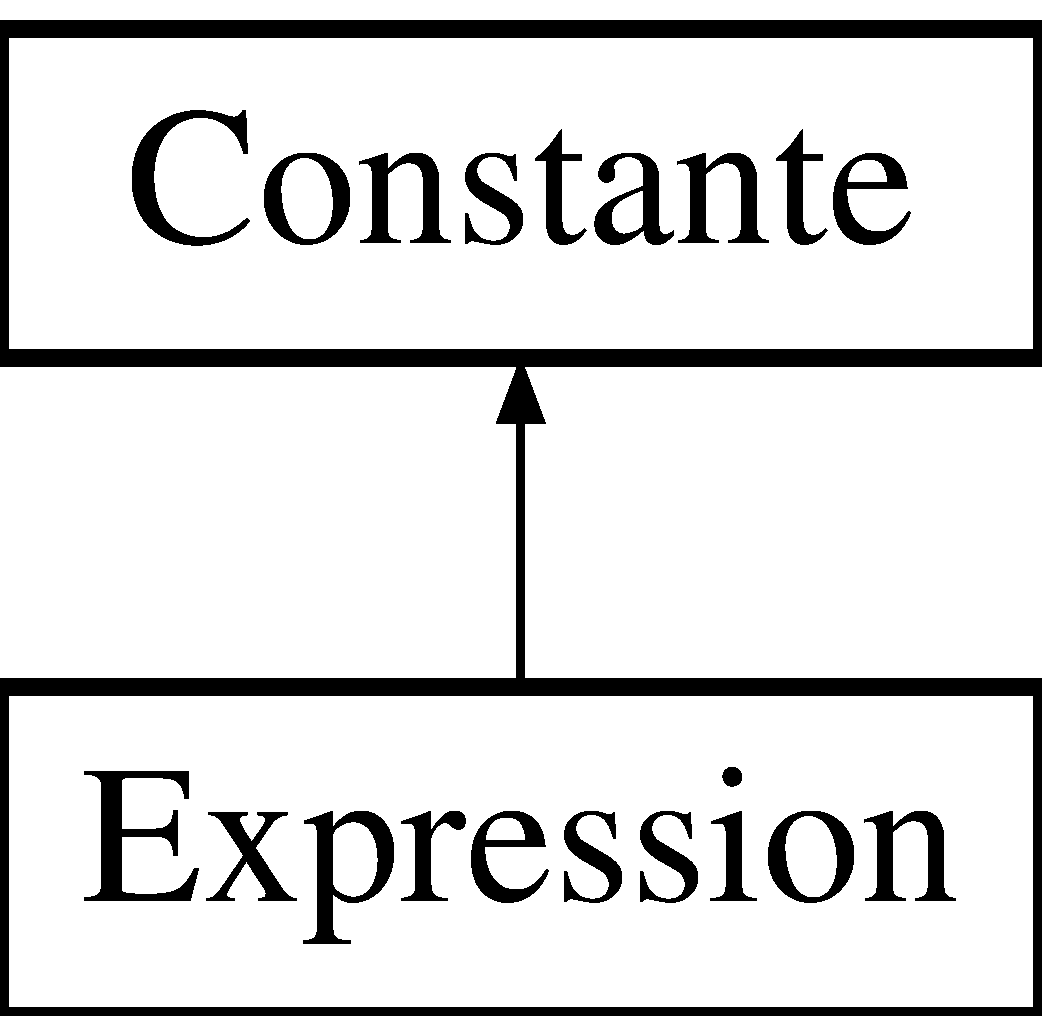
\includegraphics[height=2.000000cm]{classExpression}
\end{center}
\end{figure}
\subsection*{\-Public \-Member \-Functions}
\begin{DoxyCompactItemize}
\item 
\hyperlink{classExpression_aa235eb34251cdfe3cd9c76bb236688fe}{\-Expression} (const \-Q\-String \&s=\char`\"{}\char`\"{})
\begin{DoxyCompactList}\small\item\em \-Crée un objet de cette classe. \end{DoxyCompactList}\item 
void \hyperlink{classExpression_a1cb7bec11fe237eba6caab975f7323e7}{eval} () const 
\item 
\hyperlink{classConstante}{\-Constante} \& \hyperlink{classExpression_a1c721aa4c3ea8e860fb229f719652667}{addition} (const \hyperlink{classConstante}{\-Constante} \&n) const 
\begin{DoxyCompactList}\small\item\em \-Retourne la concatenation de l'expression encapsulée par cette classe, de la constante passée en paramètre et de l'opérateur '+'. \end{DoxyCompactList}\item 
\hyperlink{classConstante}{\-Constante} \& \hyperlink{classExpression_abd4850801886dae0b74e0c22fd45006f}{soustraction} (const \hyperlink{classConstante}{\-Constante} \&n) const 
\begin{DoxyCompactList}\small\item\em \-Retourne la concatenation de l'expression encapsulée par cette classe, de la constante passée en paramètre et de l'opérateur '-\/'. \end{DoxyCompactList}\item 
\hyperlink{classConstante}{\-Constante} \& \hyperlink{classExpression_af3b11dc48c440f08df10aa98aaf11deb}{multiplication} (const \hyperlink{classConstante}{\-Constante} \&n) const 
\begin{DoxyCompactList}\small\item\em \-Retourne la concatenation de l'expression encapsulée par cette classe, de la constante passée en paramètre et de l'opérateur '$\ast$'. \end{DoxyCompactList}\item 
\hyperlink{classConstante}{\-Constante} \& \hyperlink{classExpression_ae9b021228fe5cbbe66583784a4f9ed40}{division} (const \hyperlink{classConstante}{\-Constante} \&n) const 
\begin{DoxyCompactList}\small\item\em \-Retourne la concatenation de l'expression encapsulée par cette classe, de la constante passée en paramètre et de l'opérateur '/'. \end{DoxyCompactList}\item 
virtual \hyperlink{classExpression}{\-Expression} $\ast$ \hyperlink{classExpression_ad357e8bb1174b3582833ebcbf6d6e232}{clone} () const 
\begin{DoxyCompactList}\small\item\em \-Crée une nouvelle instance de cette classe. \-Méthode virtuelle pure héritée et implémentée depuis la classe \hyperlink{classConstante}{\-Constante}. \end{DoxyCompactList}\item 
\-Q\-String \hyperlink{classExpression_a60e6e305cdd8e878df2e3081ae15a4d0}{to\-String} () const 
\begin{DoxyCompactList}\small\item\em \-Retourne une chaine de caractères correspondant aux informations encapsulées par une expression. \-Méthode virtuelle pure héritée et implémentée depuis la classe \hyperlink{classConstante}{\-Constante}. \end{DoxyCompactList}\end{DoxyCompactItemize}


\subsection{\-Detailed \-Description}
\-Classe permettant de créer et manipuler des constantes de type \hyperlink{classExpression}{\-Expression}. \{ hérite de \hyperlink{classConstante}{\-Constante} \}. 

\subsection{\-Constructor \& \-Destructor \-Documentation}
\hypertarget{classExpression_aa235eb34251cdfe3cd9c76bb236688fe}{\index{\-Expression@{\-Expression}!\-Expression@{\-Expression}}
\index{\-Expression@{\-Expression}!Expression@{\-Expression}}
\subsubsection[{\-Expression}]{\setlength{\rightskip}{0pt plus 5cm}{\bf \-Expression\-::\-Expression} (
\begin{DoxyParamCaption}
\item[{const \-Q\-String \&}]{s = {\ttfamily \char`\"{}\char`\"{}}}
\end{DoxyParamCaption}
)\hspace{0.3cm}{\ttfamily  \mbox{[}inline\mbox{]}}}}\label{classExpression_aa235eb34251cdfe3cd9c76bb236688fe}


\-Crée un objet de cette classe. 


\begin{DoxyParams}{\-Parameters}
{\em \-Une} & chaine de caractères correspondant à l'expression.\\
\hline
\end{DoxyParams}
\-Crée un objet de cette classe. 

\subsection{\-Member \-Function \-Documentation}
\hypertarget{classExpression_a1c721aa4c3ea8e860fb229f719652667}{\index{\-Expression@{\-Expression}!addition@{addition}}
\index{addition@{addition}!Expression@{\-Expression}}
\subsubsection[{addition}]{\setlength{\rightskip}{0pt plus 5cm}{\bf \-Constante} \& {\bf \-Expression\-::addition} (
\begin{DoxyParamCaption}
\item[{const {\bf \-Constante} \&}]{n}
\end{DoxyParamCaption}
) const}}\label{classExpression_a1c721aa4c3ea8e860fb229f719652667}


\-Retourne la concatenation de l'expression encapsulée par cette classe, de la constante passée en paramètre et de l'opérateur '+'. 


\begin{DoxyParams}{\-Parameters}
{\em n} & \-La constante à concatener. \\
\hline
\end{DoxyParams}
\begin{DoxyReturn}{\-Returns}
\-Retourne la concatenation de l'expression encapsulée par cette classe, de la constante passée en paramètre et de l'opérateur '+'.
\end{DoxyReturn}
\-Retourne la concatenation de l'expression encapsulée par cette classe, de la constante passée en paramètre et de l'opérateur '+'. \hypertarget{classExpression_ad357e8bb1174b3582833ebcbf6d6e232}{\index{\-Expression@{\-Expression}!clone@{clone}}
\index{clone@{clone}!Expression@{\-Expression}}
\subsubsection[{clone}]{\setlength{\rightskip}{0pt plus 5cm}{\bf \-Expression} $\ast$ {\bf \-Expression\-::clone} (
\begin{DoxyParamCaption}
{}
\end{DoxyParamCaption}
) const\hspace{0.3cm}{\ttfamily  \mbox{[}inline, virtual\mbox{]}}}}\label{classExpression_ad357e8bb1174b3582833ebcbf6d6e232}


\-Crée une nouvelle instance de cette classe. \-Méthode virtuelle pure héritée et implémentée depuis la classe \hyperlink{classConstante}{\-Constante}. 

\begin{DoxyReturn}{\-Returns}
\-La nouvelle instance de cette classe.
\end{DoxyReturn}
\-Crée une nouvelle instance de cette classe. 

\-Implements \hyperlink{classConstante_a5769ea385161e02bd2d1bcadefc2c510}{\-Constante}.

\hypertarget{classExpression_ae9b021228fe5cbbe66583784a4f9ed40}{\index{\-Expression@{\-Expression}!division@{division}}
\index{division@{division}!Expression@{\-Expression}}
\subsubsection[{division}]{\setlength{\rightskip}{0pt plus 5cm}{\bf \-Constante} \& {\bf \-Expression\-::division} (
\begin{DoxyParamCaption}
\item[{const {\bf \-Constante} \&}]{n}
\end{DoxyParamCaption}
) const}}\label{classExpression_ae9b021228fe5cbbe66583784a4f9ed40}


\-Retourne la concatenation de l'expression encapsulée par cette classe, de la constante passée en paramètre et de l'opérateur '/'. 


\begin{DoxyParams}{\-Parameters}
{\em n} & \-La constante à concatener. \\
\hline
\end{DoxyParams}
\begin{DoxyReturn}{\-Returns}
\-Retourne la concatenation de l'expression encapsulée par cette classe, de la constante passée en paramètre et de l'opérateur '/'.
\end{DoxyReturn}
\-Retourne la concatenation de l'expression encapsulée par cette classe, de la constante passée en paramètre et de l'opérateur '/'. \hypertarget{classExpression_a1cb7bec11fe237eba6caab975f7323e7}{\index{\-Expression@{\-Expression}!eval@{eval}}
\index{eval@{eval}!Expression@{\-Expression}}
\subsubsection[{eval}]{\setlength{\rightskip}{0pt plus 5cm}void {\bf \-Expression\-::eval} (
\begin{DoxyParamCaption}
{}
\end{DoxyParamCaption}
) const}}\label{classExpression_a1cb7bec11fe237eba6caab975f7323e7}
\-Evalue l'expression encapsulée par cette classe. \hypertarget{classExpression_af3b11dc48c440f08df10aa98aaf11deb}{\index{\-Expression@{\-Expression}!multiplication@{multiplication}}
\index{multiplication@{multiplication}!Expression@{\-Expression}}
\subsubsection[{multiplication}]{\setlength{\rightskip}{0pt plus 5cm}{\bf \-Constante} \& {\bf \-Expression\-::multiplication} (
\begin{DoxyParamCaption}
\item[{const {\bf \-Constante} \&}]{n}
\end{DoxyParamCaption}
) const}}\label{classExpression_af3b11dc48c440f08df10aa98aaf11deb}


\-Retourne la concatenation de l'expression encapsulée par cette classe, de la constante passée en paramètre et de l'opérateur '$\ast$'. 


\begin{DoxyParams}{\-Parameters}
{\em n} & \-La constante à concatener. \\
\hline
\end{DoxyParams}
\begin{DoxyReturn}{\-Returns}
\-Retourne la concatenation de l'expression encapsulée par cette classe, de la constante passée en paramètre et de l'opérateur '$\ast$'.
\end{DoxyReturn}
\-Retourne la concatenation de l'expression encapsulée par cette classe, de la constante passée en paramètre et de l'opérateur '/'. \hypertarget{classExpression_abd4850801886dae0b74e0c22fd45006f}{\index{\-Expression@{\-Expression}!soustraction@{soustraction}}
\index{soustraction@{soustraction}!Expression@{\-Expression}}
\subsubsection[{soustraction}]{\setlength{\rightskip}{0pt plus 5cm}{\bf \-Constante} \& {\bf \-Expression\-::soustraction} (
\begin{DoxyParamCaption}
\item[{const {\bf \-Constante} \&}]{n}
\end{DoxyParamCaption}
) const}}\label{classExpression_abd4850801886dae0b74e0c22fd45006f}


\-Retourne la concatenation de l'expression encapsulée par cette classe, de la constante passée en paramètre et de l'opérateur '-\/'. 


\begin{DoxyParams}{\-Parameters}
{\em n} & \-La constante à concatener. \\
\hline
\end{DoxyParams}
\begin{DoxyReturn}{\-Returns}
\-Retourne la concatenation de l'expression encapsulée par cette classe, de la constante passée en paramètre et de l'opérateur '-\/'.
\end{DoxyReturn}
\-Retourne la concatenation de l'expression encapsulée par cette classe, de la constante passée en paramètre et de l'opérateur '-\/'. \hypertarget{classExpression_a60e6e305cdd8e878df2e3081ae15a4d0}{\index{\-Expression@{\-Expression}!to\-String@{to\-String}}
\index{to\-String@{to\-String}!Expression@{\-Expression}}
\subsubsection[{to\-String}]{\setlength{\rightskip}{0pt plus 5cm}\-Q\-String {\bf \-Expression\-::to\-String} (
\begin{DoxyParamCaption}
{}
\end{DoxyParamCaption}
) const\hspace{0.3cm}{\ttfamily  \mbox{[}inline, virtual\mbox{]}}}}\label{classExpression_a60e6e305cdd8e878df2e3081ae15a4d0}


\-Retourne une chaine de caractères correspondant aux informations encapsulées par une expression. \-Méthode virtuelle pure héritée et implémentée depuis la classe \hyperlink{classConstante}{\-Constante}. 

\begin{DoxyReturn}{\-Returns}
\-Une chaine de caractères correspondant aux informations encapsulées par une expression.
\end{DoxyReturn}
\-Retourne une chaine de caractères correspondant aux informations encapsulées par une expression. 

\-Implements \hyperlink{classConstante_ad5ea6850196ee9f86b74c74009a87ab1}{\-Constante}.



\-The documentation for this class was generated from the following files\-:\begin{DoxyCompactItemize}
\item 
\hyperlink{Expression_8h}{\-Expression.\-h}\item 
\-Expression.\-cpp\end{DoxyCompactItemize}

\hypertarget{classLogMessage}{\section{\-Log\-Message \-Class \-Reference}
\label{classLogMessage}\index{\-Log\-Message@{\-Log\-Message}}
}


\-Classe permettant de créer et manipuler des messages de log.  




{\ttfamily \#include $<$\-Log\-Message.\-h$>$}

\subsection*{\-Public \-Member \-Functions}
\begin{DoxyCompactItemize}
\item 
\hyperlink{classLogMessage_a4b2f72dc7a7dcdc46b719c485b48dece}{\-Log\-Message} (const \-Q\-String \&message, \hyperlink{LogMessage_8h_a1d3861c8dbb6437102a5f0d835982b80}{enum\-Importance} importance)
\begin{DoxyCompactList}\small\item\em \-Crée un objet de cette classe. \end{DoxyCompactList}\item 
std\-::string \hyperlink{classLogMessage_a48a47da01f0b389de8a7418d3c1f6671}{to\-String} ()
\begin{DoxyCompactList}\small\item\em \-Retourne une chaine de caractères correspondant aux informations encapsulées par un message de log. \end{DoxyCompactList}\end{DoxyCompactItemize}


\subsection{\-Detailed \-Description}
\-Classe permettant de créer et manipuler des messages de log. 

\subsection{\-Constructor \& \-Destructor \-Documentation}
\hypertarget{classLogMessage_a4b2f72dc7a7dcdc46b719c485b48dece}{\index{\-Log\-Message@{\-Log\-Message}!\-Log\-Message@{\-Log\-Message}}
\index{\-Log\-Message@{\-Log\-Message}!LogMessage@{\-Log\-Message}}
\subsubsection[{\-Log\-Message}]{\setlength{\rightskip}{0pt plus 5cm}{\bf \-Log\-Message\-::\-Log\-Message} (
\begin{DoxyParamCaption}
\item[{const \-Q\-String \&}]{message, }
\item[{{\bf enum\-Importance}}]{importance}
\end{DoxyParamCaption}
)}}\label{classLogMessage_a4b2f72dc7a7dcdc46b719c485b48dece}


\-Crée un objet de cette classe. 


\begin{DoxyParams}{\-Parameters}
{\em \-Une} & chaine de caractères correspondant au message de log. \\
\hline
{\em \-Un} & type enum correspondant à l'importance du message de log.\\
\hline
\end{DoxyParams}
\-Crée un objet de cette classe. 

\subsection{\-Member \-Function \-Documentation}
\hypertarget{classLogMessage_a48a47da01f0b389de8a7418d3c1f6671}{\index{\-Log\-Message@{\-Log\-Message}!to\-String@{to\-String}}
\index{to\-String@{to\-String}!LogMessage@{\-Log\-Message}}
\subsubsection[{to\-String}]{\setlength{\rightskip}{0pt plus 5cm}std\-::string {\bf \-Log\-Message\-::to\-String} (
\begin{DoxyParamCaption}
{}
\end{DoxyParamCaption}
)}}\label{classLogMessage_a48a47da01f0b389de8a7418d3c1f6671}


\-Retourne une chaine de caractères correspondant aux informations encapsulées par un message de log. 

\begin{DoxyReturn}{\-Returns}
\-Une chaine de caractères correspondant aux informations encapsulées par un message de log.
\end{DoxyReturn}
\-Retourne une chaine de caractères correspondant aux informations encapsulées par un message de log. 

\-The documentation for this class was generated from the following files\-:\begin{DoxyCompactItemize}
\item 
\hyperlink{LogMessage_8h}{\-Log\-Message.\-h}\item 
\-Log\-Message.\-cpp\end{DoxyCompactItemize}

\hypertarget{classLogSystem}{\section{\-Log\-System \-Class \-Reference}
\label{classLogSystem}\index{\-Log\-System@{\-Log\-System}}
}


\-Classe permettant d'écrire des messages de log dans un fichier spécifique.  




{\ttfamily \#include $<$\-Log\-System.\-h$>$}

\subsection*{\-Static \-Public \-Member \-Functions}
\begin{DoxyCompactItemize}
\item 
static void \hyperlink{classLogSystem_aef5c0aeb754ff25e118ca1ed14a7b5eb}{add} (\hyperlink{classLogMessage}{\-Log\-Message} log)
\begin{DoxyCompactList}\small\item\em \-Ajoute un message de log dans un fichier spécifique, et l'écrit dans la console. \end{DoxyCompactList}\item 
static void \hyperlink{classLogSystem_a003444a7d6ea5679c1380d80e51320dc}{add} (const \-Q\-String \&message, \hyperlink{LogMessage_8h_a1d3861c8dbb6437102a5f0d835982b80}{enum\-Importance} importance)
\begin{DoxyCompactList}\small\item\em \-Ajoute un message de log dans un fichier spécifique, et l'écrit dans la console. \end{DoxyCompactList}\end{DoxyCompactItemize}


\subsection{\-Detailed \-Description}
\-Classe permettant d'écrire des messages de log dans un fichier spécifique. 

\subsection{\-Member \-Function \-Documentation}
\hypertarget{classLogSystem_aef5c0aeb754ff25e118ca1ed14a7b5eb}{\index{\-Log\-System@{\-Log\-System}!add@{add}}
\index{add@{add}!LogSystem@{\-Log\-System}}
\subsubsection[{add}]{\setlength{\rightskip}{0pt plus 5cm}void {\bf \-Log\-System\-::add} (
\begin{DoxyParamCaption}
\item[{{\bf \-Log\-Message}}]{log}
\end{DoxyParamCaption}
)\hspace{0.3cm}{\ttfamily  \mbox{[}static\mbox{]}}}}\label{classLogSystem_aef5c0aeb754ff25e118ca1ed14a7b5eb}


\-Ajoute un message de log dans un fichier spécifique, et l'écrit dans la console. 


\begin{DoxyParams}{\-Parameters}
{\em log} & \-Un message de log.\\
\hline
\end{DoxyParams}
\-Ajoute un message de log dans un fichier spécifique, et l'écrit dans la console. \hypertarget{classLogSystem_a003444a7d6ea5679c1380d80e51320dc}{\index{\-Log\-System@{\-Log\-System}!add@{add}}
\index{add@{add}!LogSystem@{\-Log\-System}}
\subsubsection[{add}]{\setlength{\rightskip}{0pt plus 5cm}void {\bf \-Log\-System\-::add} (
\begin{DoxyParamCaption}
\item[{const \-Q\-String \&}]{message, }
\item[{{\bf enum\-Importance}}]{importance}
\end{DoxyParamCaption}
)\hspace{0.3cm}{\ttfamily  \mbox{[}static\mbox{]}}}}\label{classLogSystem_a003444a7d6ea5679c1380d80e51320dc}


\-Ajoute un message de log dans un fichier spécifique, et l'écrit dans la console. 


\begin{DoxyParams}{\-Parameters}
{\em message} & \-Une chaine de caractères correspondant au message de log. \\
\hline
{\em importance} & \-Un type enum correspondant à l'importance du message de log.\\
\hline
\end{DoxyParams}
\-Ajoute un message de log dans un fichier spécifique, et l'écrit dans la console. 

\-The documentation for this class was generated from the following files\-:\begin{DoxyCompactItemize}
\item 
\hyperlink{LogSystem_8h}{\-Log\-System.\-h}\item 
\-Log\-System.\-cpp\end{DoxyCompactItemize}

\hypertarget{classMainWindow}{\section{\-Main\-Window \-Class \-Reference}
\label{classMainWindow}\index{\-Main\-Window@{\-Main\-Window}}
}
\subsection*{\-Public \-Member \-Functions}
\begin{DoxyCompactItemize}
\item 
\hypertarget{classMainWindow_a8b244be8b7b7db1b08de2a2acb9409db}{{\bfseries \-Main\-Window} (\-Q\-Widget $\ast$parent=0)}\label{classMainWindow_a8b244be8b7b7db1b08de2a2acb9409db}

\item 
\hypertarget{classMainWindow_ae3d7a4598609a86e8bd317c0d85c4495}{void {\bfseries show} ()}\label{classMainWindow_ae3d7a4598609a86e8bd317c0d85c4495}

\item 
\hypertarget{classMainWindow_a430b81b3bb84b8561b4e63fe76e28c39}{void {\bfseries connections} ()}\label{classMainWindow_a430b81b3bb84b8561b4e63fe76e28c39}

\end{DoxyCompactItemize}


\-The documentation for this class was generated from the following files\-:\begin{DoxyCompactItemize}
\item 
\hyperlink{mainwindow_8h}{mainwindow.\-h}\item 
mainwindow.\-cpp\end{DoxyCompactItemize}

\hypertarget{classPile_1_1Memento}{\section{\-Pile\-:\-:\-Memento \-Class \-Reference}
\label{classPile_1_1Memento}\index{\-Pile\-::\-Memento@{\-Pile\-::\-Memento}}
}


{\ttfamily \#include $<$\-Pile.\-h$>$}

\subsection*{\-Public \-Member \-Functions}
\begin{DoxyCompactItemize}
\item 
\hyperlink{classPile_1_1Memento_a4fa4f1c31669ae315d096a81e5dad2aa}{\-Memento} (const \hyperlink{classPile}{\-Pile} $\ast$pile)
\begin{DoxyCompactList}\small\item\em \-Crée un objet de cette classe. \end{DoxyCompactList}\item 
\hyperlink{classPile}{\-Pile} $\ast$ \hyperlink{classPile_1_1Memento_a4c59910a99349a8be31ef5c10e8272ee}{get\-Pile\-Memento} () const 
\begin{DoxyCompactList}\small\item\em \-Retourne la pile courante. \end{DoxyCompactList}\end{DoxyCompactItemize}


\subsection{\-Detailed \-Description}
\-Classe permettant de toujours garder en mémoire une pile donnée. 

\subsection{\-Constructor \& \-Destructor \-Documentation}
\hypertarget{classPile_1_1Memento_a4fa4f1c31669ae315d096a81e5dad2aa}{\index{\-Pile\-::\-Memento@{\-Pile\-::\-Memento}!\-Memento@{\-Memento}}
\index{\-Memento@{\-Memento}!Pile::Memento@{\-Pile\-::\-Memento}}
\subsubsection[{\-Memento}]{\setlength{\rightskip}{0pt plus 5cm}{\bf \-Pile\-::\-Memento\-::\-Memento} (
\begin{DoxyParamCaption}
\item[{const {\bf \-Pile} $\ast$}]{pile}
\end{DoxyParamCaption}
)\hspace{0.3cm}{\ttfamily  \mbox{[}inline\mbox{]}}}}\label{classPile_1_1Memento_a4fa4f1c31669ae315d096a81e5dad2aa}


\-Crée un objet de cette classe. 


\begin{DoxyParams}{\-Parameters}
{\em \-Un} & pointeur vers une pile.\\
\hline
\end{DoxyParams}
\-Crée un objet de cette classe. 

\subsection{\-Member \-Function \-Documentation}
\hypertarget{classPile_1_1Memento_a4c59910a99349a8be31ef5c10e8272ee}{\index{\-Pile\-::\-Memento@{\-Pile\-::\-Memento}!get\-Pile\-Memento@{get\-Pile\-Memento}}
\index{get\-Pile\-Memento@{get\-Pile\-Memento}!Pile::Memento@{\-Pile\-::\-Memento}}
\subsubsection[{get\-Pile\-Memento}]{\setlength{\rightskip}{0pt plus 5cm}{\bf \-Pile}$\ast$ {\bf \-Pile\-::\-Memento\-::get\-Pile\-Memento} (
\begin{DoxyParamCaption}
{}
\end{DoxyParamCaption}
) const\hspace{0.3cm}{\ttfamily  \mbox{[}inline\mbox{]}}}}\label{classPile_1_1Memento_a4c59910a99349a8be31ef5c10e8272ee}


\-Retourne la pile courante. 

\begin{DoxyReturn}{\-Returns}
\-La pile courante.
\end{DoxyReturn}
\-Retourne la pile courante. 

\-The documentation for this class was generated from the following file\-:\begin{DoxyCompactItemize}
\item 
\hyperlink{Pile_8h}{\-Pile.\-h}\end{DoxyCompactItemize}

\hypertarget{classNombre}{\section{\-Nombre \-Class \-Reference}
\label{classNombre}\index{\-Nombre@{\-Nombre}}
}


\-Classe abstraite étant utilisée comme interface pour les classes qui en héritent. \{ hérite de \hyperlink{classConstante}{\-Constante} \}.  




{\ttfamily \#include $<$\-Nombre.\-h$>$}

\-Inheritance diagram for \-Nombre\-:\begin{figure}[H]
\begin{center}
\leavevmode
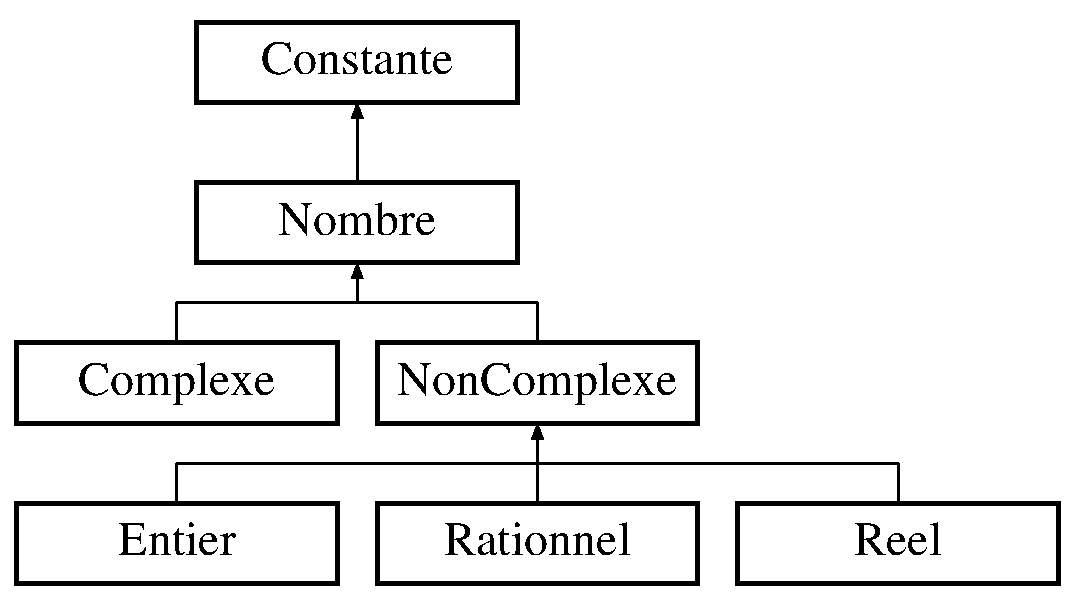
\includegraphics[height=4.000000cm]{classNombre}
\end{center}
\end{figure}
\subsection*{\-Public \-Member \-Functions}
\begin{DoxyCompactItemize}
\item 
\hyperlink{classNombre_a3c74c643475c2df0e2ecafe93a1e113a}{\-Nombre} ()
\item 
virtual \hyperlink{classNombre}{\-Nombre} \& \hyperlink{classNombre_a3fb106bcd953c9d3e03609bf1d49f2e7}{sign} () const 
\begin{DoxyCompactList}\small\item\em \-Calcule l'opposée d'un nombre. \-Méthode virtuelle. \end{DoxyCompactList}\item 
virtual \hyperlink{classNombre}{\-Nombre} \& \hyperlink{classNombre_a43b5ad781c1274196907939a36ecefcf}{sqr} () const 
\begin{DoxyCompactList}\small\item\em \-Calcule le carré d'un nombre. \-Méthode virtuelle. \end{DoxyCompactList}\item 
virtual \hyperlink{classNombre}{\-Nombre} \& \hyperlink{classNombre_a14b257b875fd98a9d53cf275464957e5}{cube} () const 
\begin{DoxyCompactList}\small\item\em \-Calcule le cube d'un nombre. \-Méthode virtuelle. \end{DoxyCompactList}\item 
\hyperlink{classNombre}{\-Nombre} \& \hyperlink{classNombre_a3e5a5aca1c59ff671feab5639ffed9b0}{operator+} (const \hyperlink{classNombre}{\-Nombre} \&n)
\begin{DoxyCompactList}\small\item\em \-Calcule la somme de deux nombres. \end{DoxyCompactList}\item 
\hyperlink{classNombre}{\-Nombre} \& \hyperlink{classNombre_a4d78f1887b4896ac59cbc66bdd919644}{operator-\/} (const \hyperlink{classNombre}{\-Nombre} \&n)
\begin{DoxyCompactList}\small\item\em \-Calcule la soustraction de deux nombres. \end{DoxyCompactList}\item 
\hyperlink{classNombre}{\-Nombre} \& \hyperlink{classNombre_a8d0fa5c9724a72a81dfb5a50f8698bad}{operator$\ast$} (const \hyperlink{classNombre}{\-Nombre} \&n)
\begin{DoxyCompactList}\small\item\em \-Calcule la multiplication de deux nombres. \end{DoxyCompactList}\item 
\hyperlink{classNombre}{\-Nombre} \& \hyperlink{classNombre_a0d46caf2a005dceb4f643a5d167d79a9}{operator/} (const \hyperlink{classNombre}{\-Nombre} \&n)
\begin{DoxyCompactList}\small\item\em \-Calcule la division de deux nombres. \end{DoxyCompactList}\item 
virtual \hyperlink{classNombre}{\-Nombre} \& \hyperlink{classNombre_ad40df43089fcb34d072b4e955a0eb4fe}{addition} (const \hyperlink{classNombre}{\-Nombre} \&nb) const =0
\begin{DoxyCompactList}\small\item\em \-Calcule la somme de deux nombres. \-Méthode virtuelle pure héritée depuis la classe \hyperlink{classNombre}{\-Nombre}. \end{DoxyCompactList}\item 
virtual \hyperlink{classNombre}{\-Nombre} \& \hyperlink{classNombre_aae525a90cd3ddeda1ce8349a23634e75}{soustraction} (const \hyperlink{classNombre}{\-Nombre} \&nb) const =0
\begin{DoxyCompactList}\small\item\em \-Calcule la soustraction de deux nombres. \-Méthode virtuelle pure héritée depuis la classe \hyperlink{classNombre}{\-Nombre}. \end{DoxyCompactList}\item 
virtual \hyperlink{classNombre}{\-Nombre} \& \hyperlink{classNombre_a742022c5e875fe24046d1c28cf043b42}{multiplication} (const \hyperlink{classNombre}{\-Nombre} \&nb) const =0
\begin{DoxyCompactList}\small\item\em \-Calcule la multiplication de deux nombres. \-Méthode virtuelle pure héritée depuis la classe \hyperlink{classNombre}{\-Nombre}. \end{DoxyCompactList}\item 
virtual \hyperlink{classNombre}{\-Nombre} \& \hyperlink{classNombre_ae4e773caee4bb349cdbe7155e26290d6}{division} (const \hyperlink{classNombre}{\-Nombre} \&nb) const =0
\begin{DoxyCompactList}\small\item\em \-Calcule la division de deux nombres. \-Méthode virtuelle pure héritée depuis la classe \hyperlink{classNombre}{\-Nombre}. \end{DoxyCompactList}\item 
virtual \hyperlink{classNombre}{\-Nombre} $\ast$ \hyperlink{classNombre_afde037df1a7545dbadb537829e90f970}{clone} () const =0
\begin{DoxyCompactList}\small\item\em \-Crée une nouvelle instance de cette classe. \-Méthode virtuelle pure héritée depuis la classe \hyperlink{classConstante}{\-Constante}. \end{DoxyCompactList}\item 
virtual \-Q\-String \hyperlink{classNombre_a8df232159bfd0e9f7e153cc73c8b128c}{to\-String} () const =0
\begin{DoxyCompactList}\small\item\em \-Retourne une chaine de caractères correspondant aux informations encapsulées par un nombre. \-Méthode virtuelle pure héritée depuis la classe \hyperlink{classConstante}{\-Constante}. \end{DoxyCompactList}\end{DoxyCompactItemize}


\subsection{\-Detailed \-Description}
\-Classe abstraite étant utilisée comme interface pour les classes qui en héritent. \{ hérite de \hyperlink{classConstante}{\-Constante} \}. 

\-Un \hyperlink{classNombre}{\-Nombre} peut être soit un \hyperlink{classComplexe}{\-Complexe} soit un \hyperlink{classNonComplexe}{\-Non\-Complexe}.

\-Le \-Design \-Pattern \-Template \-Method est utilisé. 

\subsection{\-Constructor \& \-Destructor \-Documentation}
\hypertarget{classNombre_a3c74c643475c2df0e2ecafe93a1e113a}{\index{\-Nombre@{\-Nombre}!\-Nombre@{\-Nombre}}
\index{\-Nombre@{\-Nombre}!Nombre@{\-Nombre}}
\subsubsection[{\-Nombre}]{\setlength{\rightskip}{0pt plus 5cm}{\bf \-Nombre\-::\-Nombre} (
\begin{DoxyParamCaption}
{}
\end{DoxyParamCaption}
)\hspace{0.3cm}{\ttfamily  \mbox{[}inline\mbox{]}}}}\label{classNombre_a3c74c643475c2df0e2ecafe93a1e113a}
\-Constructeur d'un nombre. 

\subsection{\-Member \-Function \-Documentation}
\hypertarget{classNombre_ad40df43089fcb34d072b4e955a0eb4fe}{\index{\-Nombre@{\-Nombre}!addition@{addition}}
\index{addition@{addition}!Nombre@{\-Nombre}}
\subsubsection[{addition}]{\setlength{\rightskip}{0pt plus 5cm}virtual {\bf \-Nombre}\& {\bf \-Nombre\-::addition} (
\begin{DoxyParamCaption}
\item[{const {\bf \-Nombre} \&}]{nb}
\end{DoxyParamCaption}
) const\hspace{0.3cm}{\ttfamily  \mbox{[}pure virtual\mbox{]}}}}\label{classNombre_ad40df43089fcb34d072b4e955a0eb4fe}


\-Calcule la somme de deux nombres. \-Méthode virtuelle pure héritée depuis la classe \hyperlink{classNombre}{\-Nombre}. 


\begin{DoxyParams}{\-Parameters}
{\em n} & \-L'autre nombre.\\
\hline
\end{DoxyParams}
\-Calcule la somme de deux nombres. 

\-Implemented in \hyperlink{classRationnel_a0b04b9aa79b75d4a9af8cb8b79f753a7}{\-Rationnel}, \hyperlink{classComplexe_a699074c8d13ed87b68aeb80463ea1379}{\-Complexe}, \hyperlink{classEntier_abbb59e17a481b81158182411a46faf82}{\-Entier}, \hyperlink{classReel_a9bad18cd80469dfb8a16900f699abf2a}{\-Reel}, and \hyperlink{classNonComplexe_a1ed6f047d5c576f03616535e3e92ab39}{\-Non\-Complexe}.

\hypertarget{classNombre_afde037df1a7545dbadb537829e90f970}{\index{\-Nombre@{\-Nombre}!clone@{clone}}
\index{clone@{clone}!Nombre@{\-Nombre}}
\subsubsection[{clone}]{\setlength{\rightskip}{0pt plus 5cm}virtual {\bf \-Nombre}$\ast$ {\bf \-Nombre\-::clone} (
\begin{DoxyParamCaption}
{}
\end{DoxyParamCaption}
) const\hspace{0.3cm}{\ttfamily  \mbox{[}inline, pure virtual\mbox{]}}}}\label{classNombre_afde037df1a7545dbadb537829e90f970}


\-Crée une nouvelle instance de cette classe. \-Méthode virtuelle pure héritée depuis la classe \hyperlink{classConstante}{\-Constante}. 

\begin{DoxyReturn}{\-Returns}
\-La nouvelle instance de cette classe.
\end{DoxyReturn}
\-Crée une nouvelle instance de cette classe. 

\-Implements \hyperlink{classConstante_a5769ea385161e02bd2d1bcadefc2c510}{\-Constante}.



\-Implemented in \hyperlink{classNonComplexe_a7f1a3881b59680f3d3a7809c75ab2138}{\-Non\-Complexe}, \hyperlink{classRationnel_a422ec3e0c4465d08c4e9deceda6c442c}{\-Rationnel}, \hyperlink{classComplexe_a7a7a8d883e959fd7d5f84d5b2b7b2a9e}{\-Complexe}, \hyperlink{classEntier_aca1eef6372c8d74274bffd435888ef57}{\-Entier}, and \hyperlink{classReel_ab53c7d10a93c702bd7ccde897fc396df}{\-Reel}.

\hypertarget{classNombre_a14b257b875fd98a9d53cf275464957e5}{\index{\-Nombre@{\-Nombre}!cube@{cube}}
\index{cube@{cube}!Nombre@{\-Nombre}}
\subsubsection[{cube}]{\setlength{\rightskip}{0pt plus 5cm}{\bf \-Nombre} \& {\bf \-Nombre\-::cube} (
\begin{DoxyParamCaption}
{}
\end{DoxyParamCaption}
) const\hspace{0.3cm}{\ttfamily  \mbox{[}virtual\mbox{]}}}}\label{classNombre_a14b257b875fd98a9d53cf275464957e5}


\-Calcule le cube d'un nombre. \-Méthode virtuelle. 

\begin{DoxyReturn}{\-Returns}
\-Le cube d'un nombre.
\end{DoxyReturn}
\-Calcule le cube d'un nombre. 

\-Reimplemented in \hyperlink{classComplexe_a1f1f8bb3f3c98b55ed934b0c8695bf2f}{\-Complexe}.

\hypertarget{classNombre_ae4e773caee4bb349cdbe7155e26290d6}{\index{\-Nombre@{\-Nombre}!division@{division}}
\index{division@{division}!Nombre@{\-Nombre}}
\subsubsection[{division}]{\setlength{\rightskip}{0pt plus 5cm}virtual {\bf \-Nombre}\& {\bf \-Nombre\-::division} (
\begin{DoxyParamCaption}
\item[{const {\bf \-Nombre} \&}]{nb}
\end{DoxyParamCaption}
) const\hspace{0.3cm}{\ttfamily  \mbox{[}pure virtual\mbox{]}}}}\label{classNombre_ae4e773caee4bb349cdbe7155e26290d6}


\-Calcule la division de deux nombres. \-Méthode virtuelle pure héritée depuis la classe \hyperlink{classNombre}{\-Nombre}. 


\begin{DoxyParams}{\-Parameters}
{\em n} & \-L'autre nombre.\\
\hline
\end{DoxyParams}
\-Calcule la division de deux nombres. 

\-Implemented in \hyperlink{classRationnel_a7797b234a41853c34db9a7bae8b77538}{\-Rationnel}, \hyperlink{classComplexe_aad8b6ff92139b04c7357a0e566926a20}{\-Complexe}, \hyperlink{classReel_a041d68cd7ee92fe30178ef1270d4628b}{\-Reel}, \hyperlink{classEntier_a968f1bd92ad6fc703aa3160921d905f7}{\-Entier}, and \hyperlink{classNonComplexe_a1af698f4c7d50e69f2c7dfa3e7998cdd}{\-Non\-Complexe}.

\hypertarget{classNombre_a742022c5e875fe24046d1c28cf043b42}{\index{\-Nombre@{\-Nombre}!multiplication@{multiplication}}
\index{multiplication@{multiplication}!Nombre@{\-Nombre}}
\subsubsection[{multiplication}]{\setlength{\rightskip}{0pt plus 5cm}virtual {\bf \-Nombre}\& {\bf \-Nombre\-::multiplication} (
\begin{DoxyParamCaption}
\item[{const {\bf \-Nombre} \&}]{nb}
\end{DoxyParamCaption}
) const\hspace{0.3cm}{\ttfamily  \mbox{[}pure virtual\mbox{]}}}}\label{classNombre_a742022c5e875fe24046d1c28cf043b42}


\-Calcule la multiplication de deux nombres. \-Méthode virtuelle pure héritée depuis la classe \hyperlink{classNombre}{\-Nombre}. 


\begin{DoxyParams}{\-Parameters}
{\em n} & \-L'autre nombre.\\
\hline
\end{DoxyParams}
\-Calcule la multiplication de deux nombres. 

\-Implemented in \hyperlink{classRationnel_a08cda12f3d5f7ed92a4a133ad2cf0b31}{\-Rationnel}, \hyperlink{classComplexe_a1137e6bfa881a8523463adf6f1f15a36}{\-Complexe}, \hyperlink{classReel_a5bdfb76995bdea709a971fa2d134de46}{\-Reel}, \hyperlink{classEntier_a4e51200ae8e5e704ecb349d2d69f0dbf}{\-Entier}, and \hyperlink{classNonComplexe_a7343c4742a895813a4b031fb67170dc8}{\-Non\-Complexe}.

\hypertarget{classNombre_a8d0fa5c9724a72a81dfb5a50f8698bad}{\index{\-Nombre@{\-Nombre}!operator$\ast$@{operator$\ast$}}
\index{operator$\ast$@{operator$\ast$}!Nombre@{\-Nombre}}
\subsubsection[{operator$\ast$}]{\setlength{\rightskip}{0pt plus 5cm}{\bf \-Nombre} \& \-Nombre\-::operator$\ast$ (
\begin{DoxyParamCaption}
\item[{const {\bf \-Nombre} \&}]{n}
\end{DoxyParamCaption}
)\hspace{0.3cm}{\ttfamily  \mbox{[}inline\mbox{]}}}}\label{classNombre_a8d0fa5c9724a72a81dfb5a50f8698bad}


\-Calcule la multiplication de deux nombres. 


\begin{DoxyParams}{\-Parameters}
{\em n} & \-L'autre nombre. \\
\hline
\end{DoxyParams}
\begin{DoxyReturn}{\-Returns}
\-La multiplication de deux nombres.
\end{DoxyReturn}
\-Calcule la multiplication de deux nombres. \hypertarget{classNombre_a3e5a5aca1c59ff671feab5639ffed9b0}{\index{\-Nombre@{\-Nombre}!operator+@{operator+}}
\index{operator+@{operator+}!Nombre@{\-Nombre}}
\subsubsection[{operator+}]{\setlength{\rightskip}{0pt plus 5cm}{\bf \-Nombre} \& \-Nombre\-::operator+ (
\begin{DoxyParamCaption}
\item[{const {\bf \-Nombre} \&}]{n}
\end{DoxyParamCaption}
)\hspace{0.3cm}{\ttfamily  \mbox{[}inline\mbox{]}}}}\label{classNombre_a3e5a5aca1c59ff671feab5639ffed9b0}


\-Calcule la somme de deux nombres. 


\begin{DoxyParams}{\-Parameters}
{\em n} & \-L'autre nombre. \\
\hline
\end{DoxyParams}
\begin{DoxyReturn}{\-Returns}
\-La somme de deux nombres.
\end{DoxyReturn}
\-Calcule la somme de deux nombres. \hypertarget{classNombre_a4d78f1887b4896ac59cbc66bdd919644}{\index{\-Nombre@{\-Nombre}!operator-\/@{operator-\/}}
\index{operator-\/@{operator-\/}!Nombre@{\-Nombre}}
\subsubsection[{operator-\/}]{\setlength{\rightskip}{0pt plus 5cm}{\bf \-Nombre} \& \-Nombre\-::operator-\/ (
\begin{DoxyParamCaption}
\item[{const {\bf \-Nombre} \&}]{n}
\end{DoxyParamCaption}
)\hspace{0.3cm}{\ttfamily  \mbox{[}inline\mbox{]}}}}\label{classNombre_a4d78f1887b4896ac59cbc66bdd919644}


\-Calcule la soustraction de deux nombres. 


\begin{DoxyParams}{\-Parameters}
{\em n} & \-L'autre nombre. \\
\hline
\end{DoxyParams}
\begin{DoxyReturn}{\-Returns}
\-La soustraction de deux nombres.
\end{DoxyReturn}
\-Calcule la soustraction de deux nombres. \hypertarget{classNombre_a0d46caf2a005dceb4f643a5d167d79a9}{\index{\-Nombre@{\-Nombre}!operator/@{operator/}}
\index{operator/@{operator/}!Nombre@{\-Nombre}}
\subsubsection[{operator/}]{\setlength{\rightskip}{0pt plus 5cm}{\bf \-Nombre} \& \-Nombre\-::operator/ (
\begin{DoxyParamCaption}
\item[{const {\bf \-Nombre} \&}]{n}
\end{DoxyParamCaption}
)\hspace{0.3cm}{\ttfamily  \mbox{[}inline\mbox{]}}}}\label{classNombre_a0d46caf2a005dceb4f643a5d167d79a9}


\-Calcule la division de deux nombres. 


\begin{DoxyParams}{\-Parameters}
{\em n} & \-L'autre nombre. \\
\hline
\end{DoxyParams}
\begin{DoxyReturn}{\-Returns}
\-La division de deux nombres.
\end{DoxyReturn}
\-Calcule la division de deux nombres. \hypertarget{classNombre_a3fb106bcd953c9d3e03609bf1d49f2e7}{\index{\-Nombre@{\-Nombre}!sign@{sign}}
\index{sign@{sign}!Nombre@{\-Nombre}}
\subsubsection[{sign}]{\setlength{\rightskip}{0pt plus 5cm}{\bf \-Nombre} \& {\bf \-Nombre\-::sign} (
\begin{DoxyParamCaption}
{}
\end{DoxyParamCaption}
) const\hspace{0.3cm}{\ttfamily  \mbox{[}virtual\mbox{]}}}}\label{classNombre_a3fb106bcd953c9d3e03609bf1d49f2e7}


\-Calcule l'opposée d'un nombre. \-Méthode virtuelle. 

\begin{DoxyReturn}{\-Returns}
\-L'opposée d'un nombre.
\end{DoxyReturn}
\-Calcule l'opposée d'un nombre. 

\-Reimplemented in \hyperlink{classComplexe_ae22fa4e15e4d048c6094ae266b6a750e}{\-Complexe}.

\hypertarget{classNombre_aae525a90cd3ddeda1ce8349a23634e75}{\index{\-Nombre@{\-Nombre}!soustraction@{soustraction}}
\index{soustraction@{soustraction}!Nombre@{\-Nombre}}
\subsubsection[{soustraction}]{\setlength{\rightskip}{0pt plus 5cm}virtual {\bf \-Nombre}\& {\bf \-Nombre\-::soustraction} (
\begin{DoxyParamCaption}
\item[{const {\bf \-Nombre} \&}]{nb}
\end{DoxyParamCaption}
) const\hspace{0.3cm}{\ttfamily  \mbox{[}pure virtual\mbox{]}}}}\label{classNombre_aae525a90cd3ddeda1ce8349a23634e75}


\-Calcule la soustraction de deux nombres. \-Méthode virtuelle pure héritée depuis la classe \hyperlink{classNombre}{\-Nombre}. 


\begin{DoxyParams}{\-Parameters}
{\em n} & \-L'autre nombre.\\
\hline
\end{DoxyParams}
\-Calcule la soustraction de deux nombres. 

\-Implemented in \hyperlink{classRationnel_a568a44d3bb7c39ec7096a939ce067f8f}{\-Rationnel}, \hyperlink{classComplexe_a54ecc525a7dc0e6491cd3125010b30bf}{\-Complexe}, \hyperlink{classEntier_aad2b72821451bf5a0445f1cccc8ab1cb}{\-Entier}, \hyperlink{classReel_a5ab824ed0b29698abbe95d0edb671f97}{\-Reel}, and \hyperlink{classNonComplexe_ac7e41f7e2f5422687985a5fe501e243f}{\-Non\-Complexe}.

\hypertarget{classNombre_a43b5ad781c1274196907939a36ecefcf}{\index{\-Nombre@{\-Nombre}!sqr@{sqr}}
\index{sqr@{sqr}!Nombre@{\-Nombre}}
\subsubsection[{sqr}]{\setlength{\rightskip}{0pt plus 5cm}{\bf \-Nombre} \& {\bf \-Nombre\-::sqr} (
\begin{DoxyParamCaption}
{}
\end{DoxyParamCaption}
) const\hspace{0.3cm}{\ttfamily  \mbox{[}virtual\mbox{]}}}}\label{classNombre_a43b5ad781c1274196907939a36ecefcf}


\-Calcule le carré d'un nombre. \-Méthode virtuelle. 

\begin{DoxyReturn}{\-Returns}
\-Le carré d'un nombre.
\end{DoxyReturn}
\-Calcule le carré d'un nombre. 

\-Reimplemented in \hyperlink{classComplexe_a4d7ad8bc647f9c3067a0093619f609c0}{\-Complexe}.

\hypertarget{classNombre_a8df232159bfd0e9f7e153cc73c8b128c}{\index{\-Nombre@{\-Nombre}!to\-String@{to\-String}}
\index{to\-String@{to\-String}!Nombre@{\-Nombre}}
\subsubsection[{to\-String}]{\setlength{\rightskip}{0pt plus 5cm}virtual \-Q\-String {\bf \-Nombre\-::to\-String} (
\begin{DoxyParamCaption}
{}
\end{DoxyParamCaption}
) const\hspace{0.3cm}{\ttfamily  \mbox{[}pure virtual\mbox{]}}}}\label{classNombre_a8df232159bfd0e9f7e153cc73c8b128c}


\-Retourne une chaine de caractères correspondant aux informations encapsulées par un nombre. \-Méthode virtuelle pure héritée depuis la classe \hyperlink{classConstante}{\-Constante}. 

\begin{DoxyReturn}{\-Returns}
\-Une chaine de caractères correspondant aux informations encapsulées par un nombre.
\end{DoxyReturn}
\-Retourne une chaine de caractères correspondant aux informations encapsulées par un nombre. 

\-Implements \hyperlink{classConstante_ad5ea6850196ee9f86b74c74009a87ab1}{\-Constante}.



\-Implemented in \hyperlink{classNonComplexe_abae1947a8f9f582f94d5e791ce4624d6}{\-Non\-Complexe}, \hyperlink{classRationnel_a41bc89d21ce161818f67ccfe296766c0}{\-Rationnel}, \hyperlink{classEntier_aa960356dfeae8af6dfa2cd25136a1a6f}{\-Entier}, \hyperlink{classReel_a990e8324822ba3dbc64fc7ff727411e2}{\-Reel}, and \hyperlink{classComplexe_a327fd83ec9743fb43c5d47831d8ed45c}{\-Complexe}.



\-The documentation for this class was generated from the following files\-:\begin{DoxyCompactItemize}
\item 
\hyperlink{Nombre_8h}{\-Nombre.\-h}\item 
\-Nombre.\-cpp\end{DoxyCompactItemize}

\hypertarget{classNonComplexe}{\section{\-Non\-Complexe \-Class \-Reference}
\label{classNonComplexe}\index{\-Non\-Complexe@{\-Non\-Complexe}}
}


\-Classe permettant de créer et manipuler des constantes de type \hyperlink{classNonComplexe}{\-Non\-Complexe}, fourni également une interface aux classes qui en héritent. \{ hérite de \hyperlink{classNombre}{\-Nombre} \}.  




{\ttfamily \#include $<$\-Non\-Complexe.\-h$>$}

\-Inheritance diagram for \-Non\-Complexe\-:\begin{figure}[H]
\begin{center}
\leavevmode
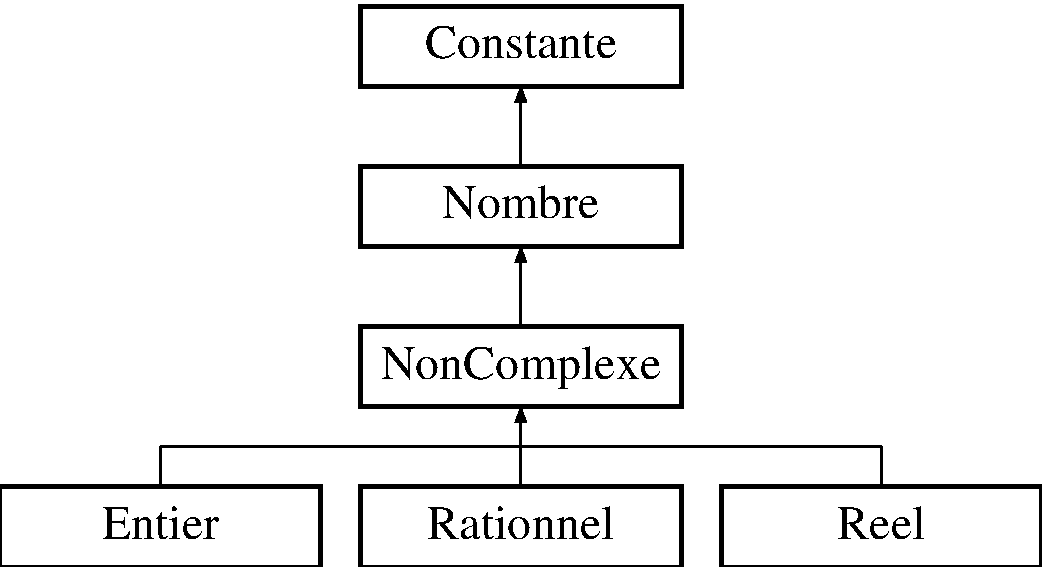
\includegraphics[height=4.000000cm]{classNonComplexe}
\end{center}
\end{figure}
\subsection*{\-Public \-Member \-Functions}
\begin{DoxyCompactItemize}
\item 
virtual \hyperlink{classNombre}{\-Nombre} \& \hyperlink{classNonComplexe_a1ed6f047d5c576f03616535e3e92ab39}{addition} (const \hyperlink{classNombre}{\-Nombre} \&n) const =0
\begin{DoxyCompactList}\small\item\em \-Calcule la somme de deux nombres. \-Méthode virtuelle pure héritée depuis la classe \hyperlink{classNombre}{\-Nombre}. \end{DoxyCompactList}\item 
virtual \hyperlink{classNombre}{\-Nombre} \& \hyperlink{classNonComplexe_ac7e41f7e2f5422687985a5fe501e243f}{soustraction} (const \hyperlink{classNombre}{\-Nombre} \&n) const =0
\begin{DoxyCompactList}\small\item\em \-Calcule la soustraction de deux nombres. \-Méthode virtuelle pure héritée depuis la classe \hyperlink{classNombre}{\-Nombre}. \end{DoxyCompactList}\item 
virtual \hyperlink{classNombre}{\-Nombre} \& \hyperlink{classNonComplexe_a7343c4742a895813a4b031fb67170dc8}{multiplication} (const \hyperlink{classNombre}{\-Nombre} \&n) const =0
\begin{DoxyCompactList}\small\item\em \-Calcule la multiplication de deux nombres. \-Méthode virtuelle pure héritée depuis la classe \hyperlink{classNombre}{\-Nombre}. \end{DoxyCompactList}\item 
virtual \hyperlink{classNombre}{\-Nombre} \& \hyperlink{classNonComplexe_a1af698f4c7d50e69f2c7dfa3e7998cdd}{division} (const \hyperlink{classNombre}{\-Nombre} \&n) const =0
\begin{DoxyCompactList}\small\item\em \-Calcule la division de deux nombres. \-Méthode virtuelle pure héritée depuis la classe \hyperlink{classNombre}{\-Nombre}. \end{DoxyCompactList}\item 
virtual \hyperlink{classNonComplexe}{\-Non\-Complexe} \& \hyperlink{classNonComplexe_af5751554285a6bf0bb1433a059bbfcdd}{to\-Entier} () const =0
\begin{DoxyCompactList}\small\item\em \-Converti le nombre non complexe en un nombre non complexe. \-Méthode virtuelle pure. \end{DoxyCompactList}\item 
virtual \hyperlink{classNonComplexe}{\-Non\-Complexe} \& \hyperlink{classNonComplexe_a0bd70b66aeb18213beb9d777287540de}{to\-Reel} () const =0
\begin{DoxyCompactList}\small\item\em \-Converti le nombre non complexe en un nombre non complexe. \-Méthode virtuelle pure. \end{DoxyCompactList}\item 
virtual \hyperlink{classNonComplexe}{\-Non\-Complexe} \& \hyperlink{classNonComplexe_a5c416e7c9d4c011c67b69b112cc30cc1}{to\-Rationnel} () const =0
\begin{DoxyCompactList}\small\item\em \-Converti le nombre non complexe en un nombre non complexe. \-Méthode virtuelle pure. \end{DoxyCompactList}\item 
virtual \hyperlink{classNonComplexe}{\-Non\-Complexe} \& \hyperlink{classNonComplexe_ad29a8407072d909cd204945d5cd5bc17}{to\-Complexe} () const =0
\begin{DoxyCompactList}\small\item\em \-Converti le nombre non complexe en un nombre non complexe. \-Méthode virtuelle pure. \end{DoxyCompactList}\item 
\hyperlink{classNonComplexe}{\-Non\-Complexe} \& \hyperlink{classNonComplexe_abf88a21ec1084e4a38cb2b5395baab6c}{sin} () const 
\begin{DoxyCompactList}\small\item\em \-Calcule le sinus du nombre non complexe. \end{DoxyCompactList}\item 
\hyperlink{classNonComplexe}{\-Non\-Complexe} \& \hyperlink{classNonComplexe_a48b17af73b9f5394bb59d092dddc84e0}{cos} () const 
\begin{DoxyCompactList}\small\item\em \-Calcule le cosinus du nombre non complexe. \end{DoxyCompactList}\item 
\hyperlink{classNonComplexe}{\-Non\-Complexe} \& \hyperlink{classNonComplexe_a76dce5128e2121dfbcda9c75d12279b2}{tan} () const 
\begin{DoxyCompactList}\small\item\em \-Calcule la tangente du nombre non complexe. \end{DoxyCompactList}\item 
\hyperlink{classNonComplexe}{\-Non\-Complexe} \& \hyperlink{classNonComplexe_aefb53599f4ea91e92f76fa66a879fe89}{sinh} () const 
\begin{DoxyCompactList}\small\item\em \-Calcule le sinus hiperbolique du nombre non complexe. \end{DoxyCompactList}\item 
\hyperlink{classNonComplexe}{\-Non\-Complexe} \& \hyperlink{classNonComplexe_a3f24a0e8d18159aee3a04c464b99a2e6}{cosh} () const 
\begin{DoxyCompactList}\small\item\em \-Calcule le cosinus hiperbolique du nombre non complexe. \end{DoxyCompactList}\item 
\hyperlink{classNonComplexe}{\-Non\-Complexe} \& \hyperlink{classNonComplexe_a6f52bc836c518adaba10464adbeb6c34}{tanh} () const 
\begin{DoxyCompactList}\small\item\em \-Calcule la tangente hiperbolique du nombre non complexe. \end{DoxyCompactList}\item 
\hyperlink{classNonComplexe}{\-Non\-Complexe} \& \hyperlink{classNonComplexe_abb6c6f03a84dfc34ee0765bd0f2e3819}{ln} () const 
\begin{DoxyCompactList}\small\item\em \-Calcule le logarithme du nombre non complexe. \end{DoxyCompactList}\item 
\hyperlink{classNonComplexe}{\-Non\-Complexe} \& \hyperlink{classNonComplexe_ad767b7dbc48a0ba68e4bc4470433ed23}{inv} () const 
\begin{DoxyCompactList}\small\item\em \-Calcule l'inverse du nombre non complexe. \end{DoxyCompactList}\item 
\hyperlink{classNonComplexe}{\-Non\-Complexe} \& \hyperlink{classNonComplexe_a9edb82d1b81fa55756bb2b4f3c19570b}{log} () const 
\begin{DoxyCompactList}\small\item\em \-Calcule le logarithme du nombre non complexe. \end{DoxyCompactList}\item 
\hyperlink{classNonComplexe}{\-Non\-Complexe} \& \hyperlink{classNonComplexe_a08f4b861f175730b81be376d8f30dcfa}{sqrt} () const 
\begin{DoxyCompactList}\small\item\em \-Calcule la racine carrée du nombre non complexe. \end{DoxyCompactList}\item 
\hyperlink{classNonComplexe}{\-Non\-Complexe} \& \hyperlink{classNonComplexe_a84716dcd2b4cd511ba6000f88e02b759}{pow} (const \hyperlink{classNonComplexe}{\-Non\-Complexe} \&puiss) const 
\begin{DoxyCompactList}\small\item\em \-Calcule la puissance passée en parametre du nombre non complexe. \end{DoxyCompactList}\item 
virtual \hyperlink{classNonComplexe}{\-Non\-Complexe} $\ast$ \hyperlink{classNonComplexe_a7f1a3881b59680f3d3a7809c75ab2138}{clone} () const =0
\begin{DoxyCompactList}\small\item\em \-Crée une nouvelle instance de cette classe. \-Méthode virtuelle pure héritée depuis la classe \hyperlink{classConstante}{\-Constante}. \end{DoxyCompactList}\item 
virtual \-Q\-String \hyperlink{classNonComplexe_abae1947a8f9f582f94d5e791ce4624d6}{to\-String} () const =0
\begin{DoxyCompactList}\small\item\em \-Retourne une chaine de caractères correspondant aux informations encapsulées par un nombre non complexe. \-Méthode virtuelle pure héritée depuis la classe \hyperlink{classConstante}{\-Constante}. \end{DoxyCompactList}\end{DoxyCompactItemize}


\subsection{\-Detailed \-Description}
\-Classe permettant de créer et manipuler des constantes de type \hyperlink{classNonComplexe}{\-Non\-Complexe}, fourni également une interface aux classes qui en héritent. \{ hérite de \hyperlink{classNombre}{\-Nombre} \}. 

\subsection{\-Member \-Function \-Documentation}
\hypertarget{classNonComplexe_a1ed6f047d5c576f03616535e3e92ab39}{\index{\-Non\-Complexe@{\-Non\-Complexe}!addition@{addition}}
\index{addition@{addition}!NonComplexe@{\-Non\-Complexe}}
\subsubsection[{addition}]{\setlength{\rightskip}{0pt plus 5cm}virtual {\bf \-Nombre}\& {\bf \-Non\-Complexe\-::addition} (
\begin{DoxyParamCaption}
\item[{const {\bf \-Nombre} \&}]{n}
\end{DoxyParamCaption}
) const\hspace{0.3cm}{\ttfamily  \mbox{[}pure virtual\mbox{]}}}}\label{classNonComplexe_a1ed6f047d5c576f03616535e3e92ab39}


\-Calcule la somme de deux nombres. \-Méthode virtuelle pure héritée depuis la classe \hyperlink{classNombre}{\-Nombre}. 


\begin{DoxyParams}{\-Parameters}
{\em n} & \-L'autre nombre.\\
\hline
\end{DoxyParams}
\-Calcule la somme de deux nombres. 

\-Implements \hyperlink{classNombre_ad40df43089fcb34d072b4e955a0eb4fe}{\-Nombre}.



\-Implemented in \hyperlink{classRationnel_a0b04b9aa79b75d4a9af8cb8b79f753a7}{\-Rationnel}, \hyperlink{classEntier_abbb59e17a481b81158182411a46faf82}{\-Entier}, and \hyperlink{classReel_a9bad18cd80469dfb8a16900f699abf2a}{\-Reel}.

\hypertarget{classNonComplexe_a7f1a3881b59680f3d3a7809c75ab2138}{\index{\-Non\-Complexe@{\-Non\-Complexe}!clone@{clone}}
\index{clone@{clone}!NonComplexe@{\-Non\-Complexe}}
\subsubsection[{clone}]{\setlength{\rightskip}{0pt plus 5cm}virtual {\bf \-Non\-Complexe}$\ast$ {\bf \-Non\-Complexe\-::clone} (
\begin{DoxyParamCaption}
{}
\end{DoxyParamCaption}
) const\hspace{0.3cm}{\ttfamily  \mbox{[}inline, pure virtual\mbox{]}}}}\label{classNonComplexe_a7f1a3881b59680f3d3a7809c75ab2138}


\-Crée une nouvelle instance de cette classe. \-Méthode virtuelle pure héritée depuis la classe \hyperlink{classConstante}{\-Constante}. 

\begin{DoxyReturn}{\-Returns}
\-La nouvelle instance de cette classe.
\end{DoxyReturn}
\-Crée une nouvelle instance de cette classe. 

\-Implements \hyperlink{classNombre_afde037df1a7545dbadb537829e90f970}{\-Nombre}.



\-Implemented in \hyperlink{classRationnel_a422ec3e0c4465d08c4e9deceda6c442c}{\-Rationnel}, \hyperlink{classEntier_aca1eef6372c8d74274bffd435888ef57}{\-Entier}, and \hyperlink{classReel_ab53c7d10a93c702bd7ccde897fc396df}{\-Reel}.

\hypertarget{classNonComplexe_a48b17af73b9f5394bb59d092dddc84e0}{\index{\-Non\-Complexe@{\-Non\-Complexe}!cos@{cos}}
\index{cos@{cos}!NonComplexe@{\-Non\-Complexe}}
\subsubsection[{cos}]{\setlength{\rightskip}{0pt plus 5cm}{\bf \-Non\-Complexe} \& {\bf \-Non\-Complexe\-::cos} (
\begin{DoxyParamCaption}
{}
\end{DoxyParamCaption}
) const}}\label{classNonComplexe_a48b17af73b9f5394bb59d092dddc84e0}


\-Calcule le cosinus du nombre non complexe. 

\begin{DoxyReturn}{\-Returns}
\-Une référence vers un nombre non complexe emmagasinant le résultat du calcul.
\end{DoxyReturn}
\-Calcule le cosinus du nombre non complexe. \hypertarget{classNonComplexe_a3f24a0e8d18159aee3a04c464b99a2e6}{\index{\-Non\-Complexe@{\-Non\-Complexe}!cosh@{cosh}}
\index{cosh@{cosh}!NonComplexe@{\-Non\-Complexe}}
\subsubsection[{cosh}]{\setlength{\rightskip}{0pt plus 5cm}{\bf \-Non\-Complexe} \& {\bf \-Non\-Complexe\-::cosh} (
\begin{DoxyParamCaption}
{}
\end{DoxyParamCaption}
) const}}\label{classNonComplexe_a3f24a0e8d18159aee3a04c464b99a2e6}


\-Calcule le cosinus hiperbolique du nombre non complexe. 

\begin{DoxyReturn}{\-Returns}
\-Une référence vers un nombre non complexe emmagasinant le résultat du calcul.
\end{DoxyReturn}
\-Calcule le cosinus hiperbolique du nombre non complexe. \hypertarget{classNonComplexe_a1af698f4c7d50e69f2c7dfa3e7998cdd}{\index{\-Non\-Complexe@{\-Non\-Complexe}!division@{division}}
\index{division@{division}!NonComplexe@{\-Non\-Complexe}}
\subsubsection[{division}]{\setlength{\rightskip}{0pt plus 5cm}virtual {\bf \-Nombre}\& {\bf \-Non\-Complexe\-::division} (
\begin{DoxyParamCaption}
\item[{const {\bf \-Nombre} \&}]{n}
\end{DoxyParamCaption}
) const\hspace{0.3cm}{\ttfamily  \mbox{[}pure virtual\mbox{]}}}}\label{classNonComplexe_a1af698f4c7d50e69f2c7dfa3e7998cdd}


\-Calcule la division de deux nombres. \-Méthode virtuelle pure héritée depuis la classe \hyperlink{classNombre}{\-Nombre}. 


\begin{DoxyParams}{\-Parameters}
{\em n} & \-L'autre nombre.\\
\hline
\end{DoxyParams}
\-Calcule la division de deux nombres. 

\-Implements \hyperlink{classNombre_ae4e773caee4bb349cdbe7155e26290d6}{\-Nombre}.



\-Implemented in \hyperlink{classRationnel_a7797b234a41853c34db9a7bae8b77538}{\-Rationnel}, \hyperlink{classReel_a041d68cd7ee92fe30178ef1270d4628b}{\-Reel}, and \hyperlink{classEntier_a968f1bd92ad6fc703aa3160921d905f7}{\-Entier}.

\hypertarget{classNonComplexe_ad767b7dbc48a0ba68e4bc4470433ed23}{\index{\-Non\-Complexe@{\-Non\-Complexe}!inv@{inv}}
\index{inv@{inv}!NonComplexe@{\-Non\-Complexe}}
\subsubsection[{inv}]{\setlength{\rightskip}{0pt plus 5cm}{\bf \-Non\-Complexe} \& {\bf \-Non\-Complexe\-::inv} (
\begin{DoxyParamCaption}
{}
\end{DoxyParamCaption}
) const}}\label{classNonComplexe_ad767b7dbc48a0ba68e4bc4470433ed23}


\-Calcule l'inverse du nombre non complexe. 

\begin{DoxyReturn}{\-Returns}
\-Une référence vers un nombre non complexe emmagasinant le résultat du calcul.
\end{DoxyReturn}
\-Calcule l'inverse du nombre non complexe. \hypertarget{classNonComplexe_abb6c6f03a84dfc34ee0765bd0f2e3819}{\index{\-Non\-Complexe@{\-Non\-Complexe}!ln@{ln}}
\index{ln@{ln}!NonComplexe@{\-Non\-Complexe}}
\subsubsection[{ln}]{\setlength{\rightskip}{0pt plus 5cm}{\bf \-Non\-Complexe} \& {\bf \-Non\-Complexe\-::ln} (
\begin{DoxyParamCaption}
{}
\end{DoxyParamCaption}
) const}}\label{classNonComplexe_abb6c6f03a84dfc34ee0765bd0f2e3819}


\-Calcule le logarithme du nombre non complexe. 

\begin{DoxyReturn}{\-Returns}
\-Une référence vers un nombre non complexe emmagasinant le résultat du calcul.
\end{DoxyReturn}
\-Calcule le logarithme du nombre non complexe. \hypertarget{classNonComplexe_a9edb82d1b81fa55756bb2b4f3c19570b}{\index{\-Non\-Complexe@{\-Non\-Complexe}!log@{log}}
\index{log@{log}!NonComplexe@{\-Non\-Complexe}}
\subsubsection[{log}]{\setlength{\rightskip}{0pt plus 5cm}{\bf \-Non\-Complexe} \& {\bf \-Non\-Complexe\-::log} (
\begin{DoxyParamCaption}
{}
\end{DoxyParamCaption}
) const}}\label{classNonComplexe_a9edb82d1b81fa55756bb2b4f3c19570b}


\-Calcule le logarithme du nombre non complexe. 

\begin{DoxyReturn}{\-Returns}
\-Une référence vers un nombre non complexe emmagasinant le résultat du calcul.
\end{DoxyReturn}
\-Calcule le logarithme du nombre non complexe. \hypertarget{classNonComplexe_a7343c4742a895813a4b031fb67170dc8}{\index{\-Non\-Complexe@{\-Non\-Complexe}!multiplication@{multiplication}}
\index{multiplication@{multiplication}!NonComplexe@{\-Non\-Complexe}}
\subsubsection[{multiplication}]{\setlength{\rightskip}{0pt plus 5cm}virtual {\bf \-Nombre}\& {\bf \-Non\-Complexe\-::multiplication} (
\begin{DoxyParamCaption}
\item[{const {\bf \-Nombre} \&}]{n}
\end{DoxyParamCaption}
) const\hspace{0.3cm}{\ttfamily  \mbox{[}pure virtual\mbox{]}}}}\label{classNonComplexe_a7343c4742a895813a4b031fb67170dc8}


\-Calcule la multiplication de deux nombres. \-Méthode virtuelle pure héritée depuis la classe \hyperlink{classNombre}{\-Nombre}. 


\begin{DoxyParams}{\-Parameters}
{\em n} & \-L'autre nombre.\\
\hline
\end{DoxyParams}
\-Calcule la multiplication de deux nombres. 

\-Implements \hyperlink{classNombre_a742022c5e875fe24046d1c28cf043b42}{\-Nombre}.



\-Implemented in \hyperlink{classRationnel_a08cda12f3d5f7ed92a4a133ad2cf0b31}{\-Rationnel}, \hyperlink{classReel_a5bdfb76995bdea709a971fa2d134de46}{\-Reel}, and \hyperlink{classEntier_a4e51200ae8e5e704ecb349d2d69f0dbf}{\-Entier}.

\hypertarget{classNonComplexe_a84716dcd2b4cd511ba6000f88e02b759}{\index{\-Non\-Complexe@{\-Non\-Complexe}!pow@{pow}}
\index{pow@{pow}!NonComplexe@{\-Non\-Complexe}}
\subsubsection[{pow}]{\setlength{\rightskip}{0pt plus 5cm}{\bf \-Non\-Complexe} \& {\bf \-Non\-Complexe\-::pow} (
\begin{DoxyParamCaption}
\item[{const {\bf \-Non\-Complexe} \&}]{puiss}
\end{DoxyParamCaption}
) const}}\label{classNonComplexe_a84716dcd2b4cd511ba6000f88e02b759}


\-Calcule la puissance passée en parametre du nombre non complexe. 


\begin{DoxyParams}{\-Parameters}
{\em \-Une} & puissance. \\
\hline
\end{DoxyParams}
\begin{DoxyReturn}{\-Returns}
\-Une référence vers un nombre non complexe emmagasinant le résultat du calcul.
\end{DoxyReturn}
\-Calcule la puissance passée en parametre du nombre non complexe. \hypertarget{classNonComplexe_abf88a21ec1084e4a38cb2b5395baab6c}{\index{\-Non\-Complexe@{\-Non\-Complexe}!sin@{sin}}
\index{sin@{sin}!NonComplexe@{\-Non\-Complexe}}
\subsubsection[{sin}]{\setlength{\rightskip}{0pt plus 5cm}{\bf \-Non\-Complexe} \& {\bf \-Non\-Complexe\-::sin} (
\begin{DoxyParamCaption}
{}
\end{DoxyParamCaption}
) const}}\label{classNonComplexe_abf88a21ec1084e4a38cb2b5395baab6c}


\-Calcule le sinus du nombre non complexe. 

\begin{DoxyReturn}{\-Returns}
\-Une référence vers un nombre non complexe emmagasinant le résultat du calcul.
\end{DoxyReturn}
\-Calcule le sinus du nombre non complexe. \hypertarget{classNonComplexe_aefb53599f4ea91e92f76fa66a879fe89}{\index{\-Non\-Complexe@{\-Non\-Complexe}!sinh@{sinh}}
\index{sinh@{sinh}!NonComplexe@{\-Non\-Complexe}}
\subsubsection[{sinh}]{\setlength{\rightskip}{0pt plus 5cm}{\bf \-Non\-Complexe} \& {\bf \-Non\-Complexe\-::sinh} (
\begin{DoxyParamCaption}
{}
\end{DoxyParamCaption}
) const}}\label{classNonComplexe_aefb53599f4ea91e92f76fa66a879fe89}


\-Calcule le sinus hiperbolique du nombre non complexe. 

\begin{DoxyReturn}{\-Returns}
\-Une référence vers un nombre non complexe emmagasinant le résultat du calcul.
\end{DoxyReturn}
\-Calcule le sinus du nombre non complexe. \hypertarget{classNonComplexe_ac7e41f7e2f5422687985a5fe501e243f}{\index{\-Non\-Complexe@{\-Non\-Complexe}!soustraction@{soustraction}}
\index{soustraction@{soustraction}!NonComplexe@{\-Non\-Complexe}}
\subsubsection[{soustraction}]{\setlength{\rightskip}{0pt plus 5cm}virtual {\bf \-Nombre}\& {\bf \-Non\-Complexe\-::soustraction} (
\begin{DoxyParamCaption}
\item[{const {\bf \-Nombre} \&}]{n}
\end{DoxyParamCaption}
) const\hspace{0.3cm}{\ttfamily  \mbox{[}pure virtual\mbox{]}}}}\label{classNonComplexe_ac7e41f7e2f5422687985a5fe501e243f}


\-Calcule la soustraction de deux nombres. \-Méthode virtuelle pure héritée depuis la classe \hyperlink{classNombre}{\-Nombre}. 


\begin{DoxyParams}{\-Parameters}
{\em n} & \-L'autre nombre.\\
\hline
\end{DoxyParams}
\-Calcule la soustraction de deux nombres. 

\-Implements \hyperlink{classNombre_aae525a90cd3ddeda1ce8349a23634e75}{\-Nombre}.



\-Implemented in \hyperlink{classRationnel_a568a44d3bb7c39ec7096a939ce067f8f}{\-Rationnel}, \hyperlink{classEntier_aad2b72821451bf5a0445f1cccc8ab1cb}{\-Entier}, and \hyperlink{classReel_a5ab824ed0b29698abbe95d0edb671f97}{\-Reel}.

\hypertarget{classNonComplexe_a08f4b861f175730b81be376d8f30dcfa}{\index{\-Non\-Complexe@{\-Non\-Complexe}!sqrt@{sqrt}}
\index{sqrt@{sqrt}!NonComplexe@{\-Non\-Complexe}}
\subsubsection[{sqrt}]{\setlength{\rightskip}{0pt plus 5cm}{\bf \-Non\-Complexe} \& {\bf \-Non\-Complexe\-::sqrt} (
\begin{DoxyParamCaption}
{}
\end{DoxyParamCaption}
) const}}\label{classNonComplexe_a08f4b861f175730b81be376d8f30dcfa}


\-Calcule la racine carrée du nombre non complexe. 

\begin{DoxyReturn}{\-Returns}
\-Une référence vers un nombre non complexe emmagasinant le résultat du calcul.
\end{DoxyReturn}
\-Calcule le racine carrée du nombre non complexe. \hypertarget{classNonComplexe_a76dce5128e2121dfbcda9c75d12279b2}{\index{\-Non\-Complexe@{\-Non\-Complexe}!tan@{tan}}
\index{tan@{tan}!NonComplexe@{\-Non\-Complexe}}
\subsubsection[{tan}]{\setlength{\rightskip}{0pt plus 5cm}{\bf \-Non\-Complexe} \& {\bf \-Non\-Complexe\-::tan} (
\begin{DoxyParamCaption}
{}
\end{DoxyParamCaption}
) const}}\label{classNonComplexe_a76dce5128e2121dfbcda9c75d12279b2}


\-Calcule la tangente du nombre non complexe. 

\begin{DoxyReturn}{\-Returns}
\-Une référence vers un nombre non complexe emmagasinant le résultat du calcul.
\end{DoxyReturn}
\-Calcule la tangente du nombre non complexe. \hypertarget{classNonComplexe_a6f52bc836c518adaba10464adbeb6c34}{\index{\-Non\-Complexe@{\-Non\-Complexe}!tanh@{tanh}}
\index{tanh@{tanh}!NonComplexe@{\-Non\-Complexe}}
\subsubsection[{tanh}]{\setlength{\rightskip}{0pt plus 5cm}{\bf \-Non\-Complexe} \& {\bf \-Non\-Complexe\-::tanh} (
\begin{DoxyParamCaption}
{}
\end{DoxyParamCaption}
) const}}\label{classNonComplexe_a6f52bc836c518adaba10464adbeb6c34}


\-Calcule la tangente hiperbolique du nombre non complexe. 

\begin{DoxyReturn}{\-Returns}
\-Une référence vers un nombre non complexe emmagasinant le résultat du calcul.
\end{DoxyReturn}
\-Calcule la tangente hiperbolique du nombre non complexe. \hypertarget{classNonComplexe_ad29a8407072d909cd204945d5cd5bc17}{\index{\-Non\-Complexe@{\-Non\-Complexe}!to\-Complexe@{to\-Complexe}}
\index{to\-Complexe@{to\-Complexe}!NonComplexe@{\-Non\-Complexe}}
\subsubsection[{to\-Complexe}]{\setlength{\rightskip}{0pt plus 5cm}virtual {\bf \-Non\-Complexe}\& {\bf \-Non\-Complexe\-::to\-Complexe} (
\begin{DoxyParamCaption}
{}
\end{DoxyParamCaption}
) const\hspace{0.3cm}{\ttfamily  \mbox{[}pure virtual\mbox{]}}}}\label{classNonComplexe_ad29a8407072d909cd204945d5cd5bc17}


\-Converti le nombre non complexe en un nombre non complexe. \-Méthode virtuelle pure. 

\begin{DoxyReturn}{\-Returns}
\-Une référence vers un nombre non complexe emmagasinant en réalité un nombre non complexe.
\end{DoxyReturn}
\-Converti le nombre non complexe en un nombre non complexe. 

\-Implemented in \hyperlink{classRationnel_a5f58000bd9f49cb352b389460e4ec7d9}{\-Rationnel}, \hyperlink{classReel_ab8195ae116be9eca6cd69b9b03a311ba}{\-Reel}, and \hyperlink{classEntier_a33148f1d942abe9f810542ae8b71e653}{\-Entier}.

\hypertarget{classNonComplexe_af5751554285a6bf0bb1433a059bbfcdd}{\index{\-Non\-Complexe@{\-Non\-Complexe}!to\-Entier@{to\-Entier}}
\index{to\-Entier@{to\-Entier}!NonComplexe@{\-Non\-Complexe}}
\subsubsection[{to\-Entier}]{\setlength{\rightskip}{0pt plus 5cm}virtual {\bf \-Non\-Complexe}\& {\bf \-Non\-Complexe\-::to\-Entier} (
\begin{DoxyParamCaption}
{}
\end{DoxyParamCaption}
) const\hspace{0.3cm}{\ttfamily  \mbox{[}pure virtual\mbox{]}}}}\label{classNonComplexe_af5751554285a6bf0bb1433a059bbfcdd}


\-Converti le nombre non complexe en un nombre non complexe. \-Méthode virtuelle pure. 

\begin{DoxyReturn}{\-Returns}
\-Une référence vers un nombre non complexe emmagasinant en réalité un nombre non complexe.
\end{DoxyReturn}
\-Converti le nombre non complexe en un nombre non complexe. 

\-Implemented in \hyperlink{classRationnel_ab828112026340067e5b938b94fcbe110}{\-Rationnel}, \hyperlink{classReel_ad9e955b349afd277bf6694aab9d928cf}{\-Reel}, and \hyperlink{classEntier_a0d34eb382eb7329b16552d191592ed27}{\-Entier}.

\hypertarget{classNonComplexe_a5c416e7c9d4c011c67b69b112cc30cc1}{\index{\-Non\-Complexe@{\-Non\-Complexe}!to\-Rationnel@{to\-Rationnel}}
\index{to\-Rationnel@{to\-Rationnel}!NonComplexe@{\-Non\-Complexe}}
\subsubsection[{to\-Rationnel}]{\setlength{\rightskip}{0pt plus 5cm}virtual {\bf \-Non\-Complexe}\& {\bf \-Non\-Complexe\-::to\-Rationnel} (
\begin{DoxyParamCaption}
{}
\end{DoxyParamCaption}
) const\hspace{0.3cm}{\ttfamily  \mbox{[}pure virtual\mbox{]}}}}\label{classNonComplexe_a5c416e7c9d4c011c67b69b112cc30cc1}


\-Converti le nombre non complexe en un nombre non complexe. \-Méthode virtuelle pure. 

\begin{DoxyReturn}{\-Returns}
\-Une référence vers un nombre non complexe emmagasinant en réalité un nombre non complexe.
\end{DoxyReturn}
\-Converti le nombre non complexe en un nombre non complexe. 

\-Implemented in \hyperlink{classRationnel_abee7f0032fc3edb4e0e4922174f988c9}{\-Rationnel}, \hyperlink{classReel_ad2c2981a8a9f140efadfef310a1c58fc}{\-Reel}, and \hyperlink{classEntier_a7a7e540ab2ea666819e6f916ed6617de}{\-Entier}.

\hypertarget{classNonComplexe_a0bd70b66aeb18213beb9d777287540de}{\index{\-Non\-Complexe@{\-Non\-Complexe}!to\-Reel@{to\-Reel}}
\index{to\-Reel@{to\-Reel}!NonComplexe@{\-Non\-Complexe}}
\subsubsection[{to\-Reel}]{\setlength{\rightskip}{0pt plus 5cm}virtual {\bf \-Non\-Complexe}\& {\bf \-Non\-Complexe\-::to\-Reel} (
\begin{DoxyParamCaption}
{}
\end{DoxyParamCaption}
) const\hspace{0.3cm}{\ttfamily  \mbox{[}pure virtual\mbox{]}}}}\label{classNonComplexe_a0bd70b66aeb18213beb9d777287540de}


\-Converti le nombre non complexe en un nombre non complexe. \-Méthode virtuelle pure. 

\begin{DoxyReturn}{\-Returns}
\-Une référence vers un nombre non complexe emmagasinant en réalité un nombre non complexe.
\end{DoxyReturn}
\-Converti le nombre non complexe en un nombre non complexe. 

\-Implemented in \hyperlink{classRationnel_aae5902c11285baa3f2a48fbb94cfa006}{\-Rationnel}, \hyperlink{classReel_a022e6e5c75053769c7fa4f8e8bfc6fa6}{\-Reel}, and \hyperlink{classEntier_a8ac645f157658a958ec4b46f9f60d3cd}{\-Entier}.

\hypertarget{classNonComplexe_abae1947a8f9f582f94d5e791ce4624d6}{\index{\-Non\-Complexe@{\-Non\-Complexe}!to\-String@{to\-String}}
\index{to\-String@{to\-String}!NonComplexe@{\-Non\-Complexe}}
\subsubsection[{to\-String}]{\setlength{\rightskip}{0pt plus 5cm}virtual \-Q\-String {\bf \-Non\-Complexe\-::to\-String} (
\begin{DoxyParamCaption}
{}
\end{DoxyParamCaption}
) const\hspace{0.3cm}{\ttfamily  \mbox{[}pure virtual\mbox{]}}}}\label{classNonComplexe_abae1947a8f9f582f94d5e791ce4624d6}


\-Retourne une chaine de caractères correspondant aux informations encapsulées par un nombre non complexe. \-Méthode virtuelle pure héritée depuis la classe \hyperlink{classConstante}{\-Constante}. 

\begin{DoxyReturn}{\-Returns}
\-Une chaine de caractères correspondant aux informations encapsulées par un nombre non complexe.
\end{DoxyReturn}
\-Retourne une chaine de caractères correspondant aux informations encapsulées par un nombre non complexe. 

\-Implements \hyperlink{classNombre_a8df232159bfd0e9f7e153cc73c8b128c}{\-Nombre}.



\-Implemented in \hyperlink{classRationnel_a41bc89d21ce161818f67ccfe296766c0}{\-Rationnel}, \hyperlink{classEntier_aa960356dfeae8af6dfa2cd25136a1a6f}{\-Entier}, and \hyperlink{classReel_a990e8324822ba3dbc64fc7ff727411e2}{\-Reel}.



\-The documentation for this class was generated from the following files\-:\begin{DoxyCompactItemize}
\item 
\hyperlink{NonComplexe_8h}{\-Non\-Complexe.\-h}\item 
\-Non\-Complexe.\-cpp\end{DoxyCompactItemize}

\hypertarget{classOperateur}{\section{\-Operateur \-Class \-Reference}
\label{classOperateur}\index{\-Operateur@{\-Operateur}}
}


\-Classe permettant de créer et manipuler des opérateurs.  




{\ttfamily \#include $<$\-Operateur.\-h$>$}

\subsection*{\-Public \-Member \-Functions}
\begin{DoxyCompactItemize}
\item 
\hyperlink{classOperateur_aa27043213a0178c8c89af8881b9606db}{\-Operateur} (const \-Q\-String \&s)
\begin{DoxyCompactList}\small\item\em \-Crée un objet de cette classe. \end{DoxyCompactList}\item 
void \hyperlink{classOperateur_ab867284af614fc85fecc8d336f4683fa}{effectuer\-Operation} () const 
\end{DoxyCompactItemize}


\subsection{\-Detailed \-Description}
\-Classe permettant de créer et manipuler des opérateurs. 

\subsection{\-Constructor \& \-Destructor \-Documentation}
\hypertarget{classOperateur_aa27043213a0178c8c89af8881b9606db}{\index{\-Operateur@{\-Operateur}!\-Operateur@{\-Operateur}}
\index{\-Operateur@{\-Operateur}!Operateur@{\-Operateur}}
\subsubsection[{\-Operateur}]{\setlength{\rightskip}{0pt plus 5cm}{\bf \-Operateur\-::\-Operateur} (
\begin{DoxyParamCaption}
\item[{const \-Q\-String \&}]{s}
\end{DoxyParamCaption}
)}}\label{classOperateur_aa27043213a0178c8c89af8881b9606db}


\-Crée un objet de cette classe. 


\begin{DoxyParams}{\-Parameters}
{\em \-Une} & chaine de caractères correspondant à l'opérateur.\\
\hline
\end{DoxyParams}
\-Crée un objet de cette classe. 

\subsection{\-Member \-Function \-Documentation}
\hypertarget{classOperateur_ab867284af614fc85fecc8d336f4683fa}{\index{\-Operateur@{\-Operateur}!effectuer\-Operation@{effectuer\-Operation}}
\index{effectuer\-Operation@{effectuer\-Operation}!Operateur@{\-Operateur}}
\subsubsection[{effectuer\-Operation}]{\setlength{\rightskip}{0pt plus 5cm}void {\bf \-Operateur\-::effectuer\-Operation} (
\begin{DoxyParamCaption}
{}
\end{DoxyParamCaption}
) const}}\label{classOperateur_ab867284af614fc85fecc8d336f4683fa}
\-Effectue l'opération encapsulée par cette classe (traitement avec la pile). 

\-The documentation for this class was generated from the following files\-:\begin{DoxyCompactItemize}
\item 
\hyperlink{Operateur_8h}{\-Operateur.\-h}\item 
\-Operateur.\-cpp\end{DoxyCompactItemize}

\hypertarget{classPile}{\section{\-Pile \-Class \-Reference}
\label{classPile}\index{\-Pile@{\-Pile}}
}


\-Classe permettant de stocker les différentes constantes et résultats de calculs de l'utilisateur de la calculatrice. \{ hérite de \-Q\-Stack$<$\-Constante$\ast$$>$ \}.  




{\ttfamily \#include $<$\-Pile.\-h$>$}

\subsection*{\-Classes}
\begin{DoxyCompactItemize}
\item 
class \hyperlink{classPile_1_1Memento}{\-Memento}
\end{DoxyCompactItemize}
\subsection*{\-Public \-Member \-Functions}
\begin{DoxyCompactItemize}
\item 
void \hyperlink{classPile_a1a19ce2a4a6a76286fae8243a1f9e247}{swap} (int x, int y)
\begin{DoxyCompactList}\small\item\em \-Effectue le swap entre les valeurs de la pile se trouvant aux positions x et y. \end{DoxyCompactList}\item 
void \hyperlink{classPile_ae09e2cf01c21b58a6c2c4efee101c158}{sum} (int x)
\begin{DoxyCompactList}\small\item\em \-Effectue la somme des x premiers élements de la pile. \end{DoxyCompactList}\item 
void \hyperlink{classPile_a1daebba5bd1d6c6d79de63728cc892a9}{mean} (int x)
\begin{DoxyCompactList}\small\item\em \-Effectue la moyenne des x premiers élements de la pile. \end{DoxyCompactList}\item 
void \hyperlink{classPile_a3bfd5edd27566980c978b9b9692dcac2}{clear\-Pile} ()
\item 
void \hyperlink{classPile_a081f7843d01cae1f0f7be7d92e46d5d2}{dup} ()
\item 
void \hyperlink{classPile_a7488ed257c6ceb16ed57a9fffb0726d5}{drop} ()
\item 
void \hyperlink{classPile_a70be33baaba88e35a7c7fb4203cd703c}{sauvegarder\-Dans\-Fichier} (int nb\-Elts\-Pile) const 
\begin{DoxyCompactList}\small\item\em \-Sauvegarde l'état de la pile dans un fichier spécifique. \end{DoxyCompactList}\item 
int \hyperlink{classPile_a5ec4b766e09cfd2fdf97b7c093609f9d}{charger\-Depuis\-Fichier} ()
\begin{DoxyCompactList}\small\item\em \-Charge l'état de la pile depuis un fichier spécifique. \end{DoxyCompactList}\item 
\hyperlink{classPile}{\-Pile} $\ast$ \hyperlink{classPile_ab5dfd21edb0870f3dc9d8ce0eaf63e65}{clone} () const 
\begin{DoxyCompactList}\small\item\em \-Crée une nouvelle instance de cette classe. \end{DoxyCompactList}\item 
\hyperlink{classPile}{\-Pile} $\ast$ \hyperlink{classPile_aeef72130e2709198369529abc2a0155e}{get\-Pile} () const 
\begin{DoxyCompactList}\small\item\em \-Retourne la pile courante. \end{DoxyCompactList}\item 
\hyperlink{classPile_1_1Memento}{\-Memento} $\ast$ \hyperlink{classPile_a5f6591defa8702b06872735d4043c754}{sauvegarder\-Pile\-Courante} () const 
\begin{DoxyCompactList}\small\item\em \-Retourne une instance d'objet de type \hyperlink{classPile_1_1Memento}{\-Memento} encapsulant une instance de pile. \end{DoxyCompactList}\item 
void \hyperlink{classPile_a14b191f65aca9842691235fd8726dd21}{charger\-Une\-Pile} (const \hyperlink{classPile_1_1Memento}{\-Memento} $\ast$m)
\begin{DoxyCompactList}\small\item\em \-Charge la pile courante par la pile encapsulée dans l'objet de type \hyperlink{classPile_1_1Memento}{\-Memento}. \end{DoxyCompactList}\end{DoxyCompactItemize}
\subsection*{\-Static \-Public \-Member \-Functions}
\begin{DoxyCompactItemize}
\item 
static \hyperlink{classPile}{\-Pile} \& \hyperlink{classPile_a8a8779a9093f6cd64c6aed57b08e93bd}{get\-Instance} ()
\begin{DoxyCompactList}\small\item\em \-Retourne l'unique instance de cette classe. \end{DoxyCompactList}\item 
static void \hyperlink{classPile_ac1c6dc99e7b12586303e980b6c44e686}{libere\-Instance} ()
\end{DoxyCompactItemize}


\subsection{\-Detailed \-Description}
\-Classe permettant de stocker les différentes constantes et résultats de calculs de l'utilisateur de la calculatrice. \{ hérite de \-Q\-Stack$<$\-Constante$\ast$$>$ \}. 

\-Le \-Design \-Pattern \-Singleton est utilisé. 

\subsection{\-Member \-Function \-Documentation}
\hypertarget{classPile_a5ec4b766e09cfd2fdf97b7c093609f9d}{\index{\-Pile@{\-Pile}!charger\-Depuis\-Fichier@{charger\-Depuis\-Fichier}}
\index{charger\-Depuis\-Fichier@{charger\-Depuis\-Fichier}!Pile@{\-Pile}}
\subsubsection[{charger\-Depuis\-Fichier}]{\setlength{\rightskip}{0pt plus 5cm}int {\bf \-Pile\-::charger\-Depuis\-Fichier} (
\begin{DoxyParamCaption}
{}
\end{DoxyParamCaption}
)}}\label{classPile_a5ec4b766e09cfd2fdf97b7c093609f9d}


\-Charge l'état de la pile depuis un fichier spécifique. 

\begin{DoxyReturn}{\-Returns}
nb\-Elts\-Pile \-Le nombre d'élements de la pile à afficher.
\end{DoxyReturn}
\-Charge l'état de la pile depuis un fichier spécifique. \hypertarget{classPile_a14b191f65aca9842691235fd8726dd21}{\index{\-Pile@{\-Pile}!charger\-Une\-Pile@{charger\-Une\-Pile}}
\index{charger\-Une\-Pile@{charger\-Une\-Pile}!Pile@{\-Pile}}
\subsubsection[{charger\-Une\-Pile}]{\setlength{\rightskip}{0pt plus 5cm}void {\bf \-Pile\-::charger\-Une\-Pile} (
\begin{DoxyParamCaption}
\item[{const {\bf \-Memento} $\ast$}]{m}
\end{DoxyParamCaption}
)\hspace{0.3cm}{\ttfamily  \mbox{[}inline\mbox{]}}}}\label{classPile_a14b191f65aca9842691235fd8726dd21}


\-Charge la pile courante par la pile encapsulée dans l'objet de type \hyperlink{classPile_1_1Memento}{\-Memento}. 


\begin{DoxyParams}{\-Parameters}
{\em m} & \-Un pointeur vers un objet de type \hyperlink{classPile_1_1Memento}{\-Memento}.\\
\hline
\end{DoxyParams}
\-Charge la pile courante par la pile encapsulée dans l'objet de type \hyperlink{classPile_1_1Memento}{\-Memento} \hypertarget{classPile_a3bfd5edd27566980c978b9b9692dcac2}{\index{\-Pile@{\-Pile}!clear\-Pile@{clear\-Pile}}
\index{clear\-Pile@{clear\-Pile}!Pile@{\-Pile}}
\subsubsection[{clear\-Pile}]{\setlength{\rightskip}{0pt plus 5cm}void {\bf \-Pile\-::clear\-Pile} (
\begin{DoxyParamCaption}
{}
\end{DoxyParamCaption}
)}}\label{classPile_a3bfd5edd27566980c978b9b9692dcac2}
\-Vide la pile. \hypertarget{classPile_ab5dfd21edb0870f3dc9d8ce0eaf63e65}{\index{\-Pile@{\-Pile}!clone@{clone}}
\index{clone@{clone}!Pile@{\-Pile}}
\subsubsection[{clone}]{\setlength{\rightskip}{0pt plus 5cm}{\bf \-Pile} $\ast$ {\bf \-Pile\-::clone} (
\begin{DoxyParamCaption}
{}
\end{DoxyParamCaption}
) const}}\label{classPile_ab5dfd21edb0870f3dc9d8ce0eaf63e65}


\-Crée une nouvelle instance de cette classe. 

\begin{DoxyReturn}{\-Returns}
\-La nouvelle instance de cette classe.
\end{DoxyReturn}
\-Crée une nouvelle instance de cette classe. \hypertarget{classPile_a7488ed257c6ceb16ed57a9fffb0726d5}{\index{\-Pile@{\-Pile}!drop@{drop}}
\index{drop@{drop}!Pile@{\-Pile}}
\subsubsection[{drop}]{\setlength{\rightskip}{0pt plus 5cm}void {\bf \-Pile\-::drop} (
\begin{DoxyParamCaption}
{}
\end{DoxyParamCaption}
)}}\label{classPile_a7488ed257c6ceb16ed57a9fffb0726d5}
\-Supprime le dernier élement de la pile. \hypertarget{classPile_a081f7843d01cae1f0f7be7d92e46d5d2}{\index{\-Pile@{\-Pile}!dup@{dup}}
\index{dup@{dup}!Pile@{\-Pile}}
\subsubsection[{dup}]{\setlength{\rightskip}{0pt plus 5cm}void {\bf \-Pile\-::dup} (
\begin{DoxyParamCaption}
{}
\end{DoxyParamCaption}
)}}\label{classPile_a081f7843d01cae1f0f7be7d92e46d5d2}
\-Duplique le dernier élement de la pile. \hypertarget{classPile_a8a8779a9093f6cd64c6aed57b08e93bd}{\index{\-Pile@{\-Pile}!get\-Instance@{get\-Instance}}
\index{get\-Instance@{get\-Instance}!Pile@{\-Pile}}
\subsubsection[{get\-Instance}]{\setlength{\rightskip}{0pt plus 5cm}{\bf \-Pile} \& {\bf \-Pile\-::get\-Instance} (
\begin{DoxyParamCaption}
{}
\end{DoxyParamCaption}
)\hspace{0.3cm}{\ttfamily  \mbox{[}static\mbox{]}}}}\label{classPile_a8a8779a9093f6cd64c6aed57b08e93bd}


\-Retourne l'unique instance de cette classe. 

\begin{DoxyReturn}{\-Returns}
\-Un pointeur vers l'unique instance de cette classe.
\end{DoxyReturn}
\-Retourne l'unique instance de cette classe. \hypertarget{classPile_aeef72130e2709198369529abc2a0155e}{\index{\-Pile@{\-Pile}!get\-Pile@{get\-Pile}}
\index{get\-Pile@{get\-Pile}!Pile@{\-Pile}}
\subsubsection[{get\-Pile}]{\setlength{\rightskip}{0pt plus 5cm}{\bf \-Pile}$\ast$ {\bf \-Pile\-::get\-Pile} (
\begin{DoxyParamCaption}
{}
\end{DoxyParamCaption}
) const\hspace{0.3cm}{\ttfamily  \mbox{[}inline\mbox{]}}}}\label{classPile_aeef72130e2709198369529abc2a0155e}


\-Retourne la pile courante. 

\begin{DoxyReturn}{\-Returns}
\-La pile courante.
\end{DoxyReturn}
\-Retourne la pile courante. \hypertarget{classPile_ac1c6dc99e7b12586303e980b6c44e686}{\index{\-Pile@{\-Pile}!libere\-Instance@{libere\-Instance}}
\index{libere\-Instance@{libere\-Instance}!Pile@{\-Pile}}
\subsubsection[{libere\-Instance}]{\setlength{\rightskip}{0pt plus 5cm}void {\bf \-Pile\-::libere\-Instance} (
\begin{DoxyParamCaption}
{}
\end{DoxyParamCaption}
)\hspace{0.3cm}{\ttfamily  \mbox{[}static\mbox{]}}}}\label{classPile_ac1c6dc99e7b12586303e980b6c44e686}
\-Libère l'unique instance de cette classe. \hypertarget{classPile_a1daebba5bd1d6c6d79de63728cc892a9}{\index{\-Pile@{\-Pile}!mean@{mean}}
\index{mean@{mean}!Pile@{\-Pile}}
\subsubsection[{mean}]{\setlength{\rightskip}{0pt plus 5cm}void {\bf \-Pile\-::mean} (
\begin{DoxyParamCaption}
\item[{int}]{x}
\end{DoxyParamCaption}
)}}\label{classPile_a1daebba5bd1d6c6d79de63728cc892a9}


\-Effectue la moyenne des x premiers élements de la pile. 


\begin{DoxyParams}{\-Parameters}
{\em x} & \hyperlink{classNombre}{\-Nombre} d'élements de la pile pour lesquels il faut faire la moyenne.\\
\hline
\end{DoxyParams}
\-Effectue la moyenne des x premiers élements de la pile. \hypertarget{classPile_a70be33baaba88e35a7c7fb4203cd703c}{\index{\-Pile@{\-Pile}!sauvegarder\-Dans\-Fichier@{sauvegarder\-Dans\-Fichier}}
\index{sauvegarder\-Dans\-Fichier@{sauvegarder\-Dans\-Fichier}!Pile@{\-Pile}}
\subsubsection[{sauvegarder\-Dans\-Fichier}]{\setlength{\rightskip}{0pt plus 5cm}void {\bf \-Pile\-::sauvegarder\-Dans\-Fichier} (
\begin{DoxyParamCaption}
\item[{int}]{nb\-Elts\-Pile}
\end{DoxyParamCaption}
) const}}\label{classPile_a70be33baaba88e35a7c7fb4203cd703c}


\-Sauvegarde l'état de la pile dans un fichier spécifique. 


\begin{DoxyParams}{\-Parameters}
{\em nb\-Elts\-Pile} & \-Le nombre d'élements de la pile à afficher.\\
\hline
\end{DoxyParams}
\-Sauvegarde l'état de la pile dans un fichier spécifique. \hypertarget{classPile_a5f6591defa8702b06872735d4043c754}{\index{\-Pile@{\-Pile}!sauvegarder\-Pile\-Courante@{sauvegarder\-Pile\-Courante}}
\index{sauvegarder\-Pile\-Courante@{sauvegarder\-Pile\-Courante}!Pile@{\-Pile}}
\subsubsection[{sauvegarder\-Pile\-Courante}]{\setlength{\rightskip}{0pt plus 5cm}{\bf \-Memento}$\ast$ {\bf \-Pile\-::sauvegarder\-Pile\-Courante} (
\begin{DoxyParamCaption}
{}
\end{DoxyParamCaption}
) const\hspace{0.3cm}{\ttfamily  \mbox{[}inline\mbox{]}}}}\label{classPile_a5f6591defa8702b06872735d4043c754}


\-Retourne une instance d'objet de type \hyperlink{classPile_1_1Memento}{\-Memento} encapsulant une instance de pile. 

\begin{DoxyReturn}{\-Returns}
\-Un pointeur vers un objet de type \hyperlink{classPile_1_1Memento}{\-Memento}.
\end{DoxyReturn}
\-Retourne une instance d'objet de type \hyperlink{classPile_1_1Memento}{\-Memento} encapsulant une instance de pile. \hypertarget{classPile_ae09e2cf01c21b58a6c2c4efee101c158}{\index{\-Pile@{\-Pile}!sum@{sum}}
\index{sum@{sum}!Pile@{\-Pile}}
\subsubsection[{sum}]{\setlength{\rightskip}{0pt plus 5cm}void {\bf \-Pile\-::sum} (
\begin{DoxyParamCaption}
\item[{int}]{x}
\end{DoxyParamCaption}
)}}\label{classPile_ae09e2cf01c21b58a6c2c4efee101c158}


\-Effectue la somme des x premiers élements de la pile. 


\begin{DoxyParams}{\-Parameters}
{\em x} & \hyperlink{classNombre}{\-Nombre} d'élements de la pile à sommer.\\
\hline
\end{DoxyParams}
\-Effectue la somme des x premiers élements de la pile. \hypertarget{classPile_a1a19ce2a4a6a76286fae8243a1f9e247}{\index{\-Pile@{\-Pile}!swap@{swap}}
\index{swap@{swap}!Pile@{\-Pile}}
\subsubsection[{swap}]{\setlength{\rightskip}{0pt plus 5cm}void {\bf \-Pile\-::swap} (
\begin{DoxyParamCaption}
\item[{int}]{x, }
\item[{int}]{y}
\end{DoxyParamCaption}
)}}\label{classPile_a1a19ce2a4a6a76286fae8243a1f9e247}


\-Effectue le swap entre les valeurs de la pile se trouvant aux positions x et y. 


\begin{DoxyParams}{\-Parameters}
{\em x} & \-Premier indice à swaper \\
\hline
{\em y} & \-Second indice à swaper\\
\hline
\end{DoxyParams}
\-Effectue le swap entre les valeurs de la pile se trouvant aux positions x et y. 

\-The documentation for this class was generated from the following files\-:\begin{DoxyCompactItemize}
\item 
\hyperlink{Pile_8h}{\-Pile.\-h}\item 
\-Pile.\-cpp\end{DoxyCompactItemize}

\hypertarget{classPileAffichage}{\section{\-Pile\-Affichage \-Class \-Reference}
\label{classPileAffichage}\index{\-Pile\-Affichage@{\-Pile\-Affichage}}
}


\-Classe permettant de stocker les différentes constantes et résultats de calculs de l'utilisateur de la calculatrice, mais également les opérateurs. \{ hérite de \-Q\-Stack$<$\-Q\-String$>$ \}.  




{\ttfamily \#include $<$\-Pile\-Affichage.\-h$>$}

\subsection*{\-Static \-Public \-Member \-Functions}
\begin{DoxyCompactItemize}
\item 
static \hyperlink{classPileAffichage}{\-Pile\-Affichage} \& \hyperlink{classPileAffichage_a2c59a96af4c61a158f3ad84921387b00}{get\-Instance} ()
\begin{DoxyCompactList}\small\item\em \-Retourne l'unique instance de cette classe. \end{DoxyCompactList}\item 
static void \hyperlink{classPileAffichage_a5913bc068f642bdd1d376538b9caefe7}{libere\-Instance} ()
\end{DoxyCompactItemize}


\subsection{\-Detailed \-Description}
\-Classe permettant de stocker les différentes constantes et résultats de calculs de l'utilisateur de la calculatrice, mais également les opérateurs. \{ hérite de \-Q\-Stack$<$\-Q\-String$>$ \}. 

\-Le \-Design \-Pattern \-Singleton est utilisé. 

\subsection{\-Member \-Function \-Documentation}
\hypertarget{classPileAffichage_a2c59a96af4c61a158f3ad84921387b00}{\index{\-Pile\-Affichage@{\-Pile\-Affichage}!get\-Instance@{get\-Instance}}
\index{get\-Instance@{get\-Instance}!PileAffichage@{\-Pile\-Affichage}}
\subsubsection[{get\-Instance}]{\setlength{\rightskip}{0pt plus 5cm}{\bf \-Pile\-Affichage} \& {\bf \-Pile\-Affichage\-::get\-Instance} (
\begin{DoxyParamCaption}
{}
\end{DoxyParamCaption}
)\hspace{0.3cm}{\ttfamily  \mbox{[}static\mbox{]}}}}\label{classPileAffichage_a2c59a96af4c61a158f3ad84921387b00}


\-Retourne l'unique instance de cette classe. 

\begin{DoxyReturn}{\-Returns}
\-Un pointeur vers l'unique instance de cette classe.
\end{DoxyReturn}
\-Retourne l'unique instance de cette classe. \hypertarget{classPileAffichage_a5913bc068f642bdd1d376538b9caefe7}{\index{\-Pile\-Affichage@{\-Pile\-Affichage}!libere\-Instance@{libere\-Instance}}
\index{libere\-Instance@{libere\-Instance}!PileAffichage@{\-Pile\-Affichage}}
\subsubsection[{libere\-Instance}]{\setlength{\rightskip}{0pt plus 5cm}void {\bf \-Pile\-Affichage\-::libere\-Instance} (
\begin{DoxyParamCaption}
{}
\end{DoxyParamCaption}
)\hspace{0.3cm}{\ttfamily  \mbox{[}static\mbox{]}}}}\label{classPileAffichage_a5913bc068f642bdd1d376538b9caefe7}
\-Libère l'unique instance de cette classe. 

\-The documentation for this class was generated from the following files\-:\begin{DoxyCompactItemize}
\item 
\hyperlink{PileAffichage_8h}{\-Pile\-Affichage.\-h}\item 
\-Pile\-Affichage.\-cpp\end{DoxyCompactItemize}

\hypertarget{classRationnel}{\section{\-Rationnel \-Class \-Reference}
\label{classRationnel}\index{\-Rationnel@{\-Rationnel}}
}


\-Classe permettant de créer et manipuler des constantes de type \hyperlink{classRationnel}{\-Rationnel}. \{ hérite de \hyperlink{classNonComplexe}{\-Non\-Complexe} \}.  




{\ttfamily \#include $<$\-Rationnel.\-h$>$}

\-Inheritance diagram for \-Rationnel\-:\begin{figure}[H]
\begin{center}
\leavevmode
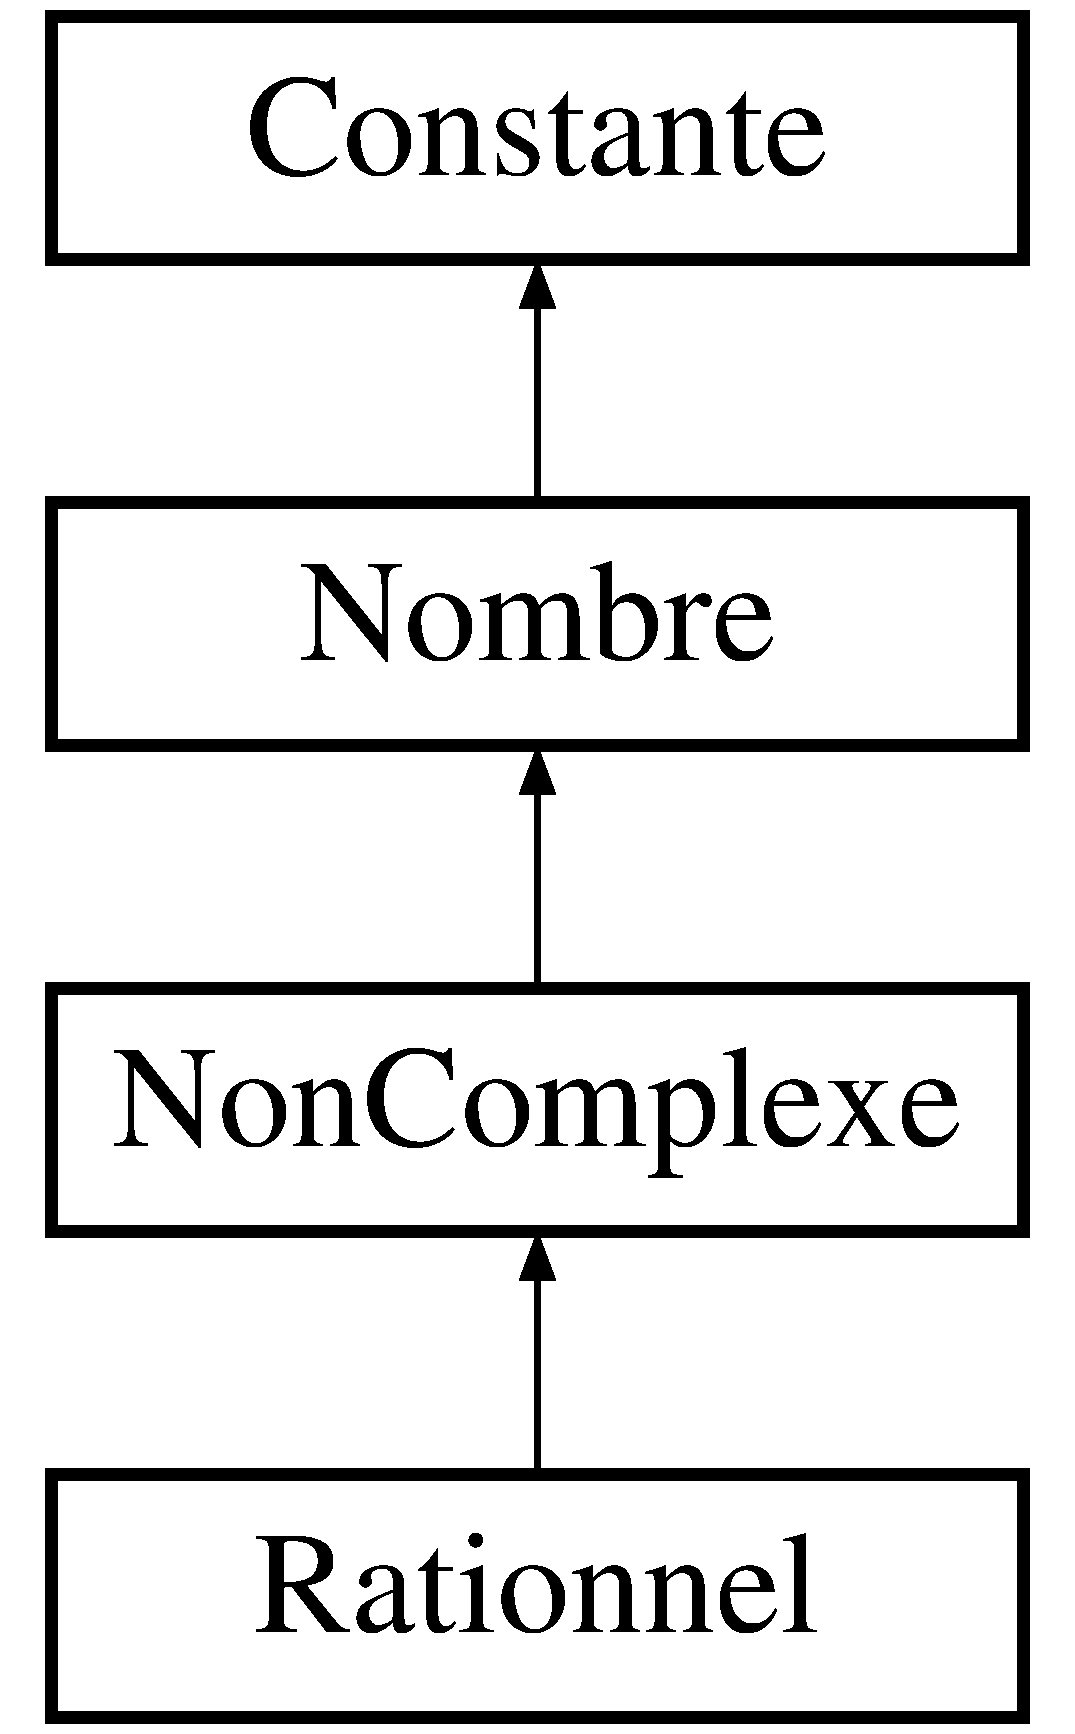
\includegraphics[height=4.000000cm]{classRationnel}
\end{center}
\end{figure}
\subsection*{\-Public \-Member \-Functions}
\begin{DoxyCompactItemize}
\item 
\hyperlink{classRationnel_a4a0ffcb25f5a20c6dc4da18c0c80110d}{\-Rationnel} (const \hyperlink{classEntier}{\-Entier} \&num, const \hyperlink{classEntier}{\-Entier} \&den)
\begin{DoxyCompactList}\small\item\em \-Crée un nombre rationnel. \end{DoxyCompactList}\item 
\hyperlink{classRationnel_aa60d0952f71e99dded642d42e9dffa3f}{\-Rationnel} (const \hyperlink{classNonComplexe}{\-Non\-Complexe} \&num, const \hyperlink{classNonComplexe}{\-Non\-Complexe} \&den)
\begin{DoxyCompactList}\small\item\em \-Crée un nombre rationnel. \end{DoxyCompactList}\item 
\hyperlink{classRationnel_ab5ce094e3a57591f7b7fa6f634490d24}{\-Rationnel} (unsigned int num=0, unsigned int den=1)
\begin{DoxyCompactList}\small\item\em \-Crée un nombre rationnel. \end{DoxyCompactList}\item 
\hyperlink{classRationnel_ab0257aa2fd1b258506ec6d2a268612c6}{$\sim$\-Rationnel} ()
\item 
\hyperlink{classNombre}{\-Nombre} \& \hyperlink{classRationnel_a0b04b9aa79b75d4a9af8cb8b79f753a7}{addition} (const \hyperlink{classNombre}{\-Nombre} \&n) const 
\begin{DoxyCompactList}\small\item\em \-Calcule la somme de ce nombre rationnel et d'un nombre. \-Méthode virtuelle pure héritée et implémentée depuis la classe \hyperlink{classNombre}{\-Nombre}. \end{DoxyCompactList}\item 
\hyperlink{classNombre}{\-Nombre} \& \hyperlink{classRationnel_a568a44d3bb7c39ec7096a939ce067f8f}{soustraction} (const \hyperlink{classNombre}{\-Nombre} \&n) const 
\begin{DoxyCompactList}\small\item\em \-Calcule la soustraction de ce nombre rationnel et d'un nombre. \-Méthode virtuelle pure héritée et implémentée depuis la classe \hyperlink{classNombre}{\-Nombre}. \end{DoxyCompactList}\item 
\hyperlink{classNombre}{\-Nombre} \& \hyperlink{classRationnel_a08cda12f3d5f7ed92a4a133ad2cf0b31}{multiplication} (const \hyperlink{classNombre}{\-Nombre} \&n) const 
\begin{DoxyCompactList}\small\item\em \-Calcule la multiplication de ce nombre rationnel et d'un nombre. \-Méthode virtuelle pure héritée et implémentée depuis la classe \hyperlink{classNombre}{\-Nombre}. \end{DoxyCompactList}\item 
\hyperlink{classNombre}{\-Nombre} \& \hyperlink{classRationnel_a7797b234a41853c34db9a7bae8b77538}{division} (const \hyperlink{classNombre}{\-Nombre} \&n) const 
\begin{DoxyCompactList}\small\item\em \-Calcule la division de ce nombre rationnel et d'un nombre. \-Méthode virtuelle pure héritée et implémentée depuis la classe \hyperlink{classNombre}{\-Nombre}. \end{DoxyCompactList}\item 
\hyperlink{classNonComplexe}{\-Non\-Complexe} \& \hyperlink{classRationnel_ab828112026340067e5b938b94fcbe110}{to\-Entier} () const 
\begin{DoxyCompactList}\small\item\em \-Converti le nombre rationnel en un nombre entier. \-Méthode virtuelle pure héritée et implémentée depuis la classe \hyperlink{classNonComplexe}{\-Non\-Complexe}. \end{DoxyCompactList}\item 
\hyperlink{classNonComplexe}{\-Non\-Complexe} \& \hyperlink{classRationnel_aae5902c11285baa3f2a48fbb94cfa006}{to\-Reel} () const 
\begin{DoxyCompactList}\small\item\em \-Converti le nombre rationnel en un nombre réel. \-Méthode virtuelle pure héritée et implémentée depuis la classe \hyperlink{classNonComplexe}{\-Non\-Complexe}. \end{DoxyCompactList}\item 
\hyperlink{classNonComplexe}{\-Non\-Complexe} \& \hyperlink{classRationnel_abee7f0032fc3edb4e0e4922174f988c9}{to\-Rationnel} () const 
\begin{DoxyCompactList}\small\item\em \-Converti le nombre rationnel en un nombre rationnel. \-Méthode virtuelle pure héritée et implémentée depuis la classe \hyperlink{classNonComplexe}{\-Non\-Complexe}. \end{DoxyCompactList}\item 
\hyperlink{classNonComplexe}{\-Non\-Complexe} \& \hyperlink{classRationnel_a5f58000bd9f49cb352b389460e4ec7d9}{to\-Complexe} () const 
\begin{DoxyCompactList}\small\item\em \-Converti le nombre rationnel en un nombre complexe. \-Méthode virtuelle pure héritée et implémentée depuis la classe \hyperlink{classNonComplexe}{\-Non\-Complexe}. \end{DoxyCompactList}\item 
void \hyperlink{classRationnel_a12ee060e5fca5f4291b222983d727268}{simplifier} ()
\item 
const \hyperlink{classEntier}{\-Entier} \& \hyperlink{classRationnel_aace94cd795afce78654255e32d627910}{get\-Num} () const 
\begin{DoxyCompactList}\small\item\em \-Retourne le numérateur de ce nombre rationnel. \end{DoxyCompactList}\item 
const \hyperlink{classEntier}{\-Entier} \& \hyperlink{classRationnel_aa0a393337f84b8aa3f1fa8958b551d7e}{get\-Den} () const 
\begin{DoxyCompactList}\small\item\em \-Retourne le dénominateur de ce nombre rationnel. \end{DoxyCompactList}\item 
virtual \hyperlink{classRationnel}{\-Rationnel} $\ast$ \hyperlink{classRationnel_a422ec3e0c4465d08c4e9deceda6c442c}{clone} () const 
\begin{DoxyCompactList}\small\item\em \-Crée une nouvelle instance de cette classe. \-Méthode virtuelle pure héritée et implémentée depuis la classe \hyperlink{classConstante}{\-Constante}. \end{DoxyCompactList}\item 
\-Q\-String \hyperlink{classRationnel_a41bc89d21ce161818f67ccfe296766c0}{to\-String} () const 
\begin{DoxyCompactList}\small\item\em \-Retourne une chaine de caractères correspondant aux informations encapsulées par un nombre rationnel. \-Méthode virtuelle pure héritée et implémentée depuis la classe \hyperlink{classConstante}{\-Constante}. \end{DoxyCompactList}\end{DoxyCompactItemize}


\subsection{\-Detailed \-Description}
\-Classe permettant de créer et manipuler des constantes de type \hyperlink{classRationnel}{\-Rationnel}. \{ hérite de \hyperlink{classNonComplexe}{\-Non\-Complexe} \}. 

\subsection{\-Constructor \& \-Destructor \-Documentation}
\hypertarget{classRationnel_a4a0ffcb25f5a20c6dc4da18c0c80110d}{\index{\-Rationnel@{\-Rationnel}!\-Rationnel@{\-Rationnel}}
\index{\-Rationnel@{\-Rationnel}!Rationnel@{\-Rationnel}}
\subsubsection[{\-Rationnel}]{\setlength{\rightskip}{0pt plus 5cm}{\bf \-Rationnel\-::\-Rationnel} (
\begin{DoxyParamCaption}
\item[{const {\bf \-Entier} \&}]{num, }
\item[{const {\bf \-Entier} \&}]{den}
\end{DoxyParamCaption}
)}}\label{classRationnel_a4a0ffcb25f5a20c6dc4da18c0c80110d}


\-Crée un nombre rationnel. 


\begin{DoxyParams}{\-Parameters}
{\em num} & \-Le numérateur de ce nombre rationnel. \\
\hline
{\em den} & \-Le dénominateur de ce nombre rationnel.\\
\hline
\end{DoxyParams}
\-Crée un nombre rationnel. \hypertarget{classRationnel_aa60d0952f71e99dded642d42e9dffa3f}{\index{\-Rationnel@{\-Rationnel}!\-Rationnel@{\-Rationnel}}
\index{\-Rationnel@{\-Rationnel}!Rationnel@{\-Rationnel}}
\subsubsection[{\-Rationnel}]{\setlength{\rightskip}{0pt plus 5cm}{\bf \-Rationnel\-::\-Rationnel} (
\begin{DoxyParamCaption}
\item[{const {\bf \-Non\-Complexe} \&}]{num, }
\item[{const {\bf \-Non\-Complexe} \&}]{den}
\end{DoxyParamCaption}
)}}\label{classRationnel_aa60d0952f71e99dded642d42e9dffa3f}


\-Crée un nombre rationnel. 


\begin{DoxyParams}{\-Parameters}
{\em num} & \-Le numérateur de ce nombre rationnel. \\
\hline
{\em den} & \-Le dénominateur de ce nombre rationnel.\\
\hline
\end{DoxyParams}
\-Crée un nombre rationnel. \hypertarget{classRationnel_ab5ce094e3a57591f7b7fa6f634490d24}{\index{\-Rationnel@{\-Rationnel}!\-Rationnel@{\-Rationnel}}
\index{\-Rationnel@{\-Rationnel}!Rationnel@{\-Rationnel}}
\subsubsection[{\-Rationnel}]{\setlength{\rightskip}{0pt plus 5cm}{\bf \-Rationnel\-::\-Rationnel} (
\begin{DoxyParamCaption}
\item[{unsigned int}]{num = {\ttfamily 0}, }
\item[{unsigned int}]{den = {\ttfamily 1}}
\end{DoxyParamCaption}
)}}\label{classRationnel_ab5ce094e3a57591f7b7fa6f634490d24}


\-Crée un nombre rationnel. 


\begin{DoxyParams}{\-Parameters}
{\em num} & \-Le numérateur de ce nombre rationnel. \\
\hline
{\em den} & \-Le dénominateur de ce nombre rationnel.\\
\hline
\end{DoxyParams}
\-Crée un nombre rationnel. \hypertarget{classRationnel_ab0257aa2fd1b258506ec6d2a268612c6}{\index{\-Rationnel@{\-Rationnel}!$\sim$\-Rationnel@{$\sim$\-Rationnel}}
\index{$\sim$\-Rationnel@{$\sim$\-Rationnel}!Rationnel@{\-Rationnel}}
\subsubsection[{$\sim$\-Rationnel}]{\setlength{\rightskip}{0pt plus 5cm}{\bf \-Rationnel\-::$\sim$\-Rationnel} (
\begin{DoxyParamCaption}
{}
\end{DoxyParamCaption}
)}}\label{classRationnel_ab0257aa2fd1b258506ec6d2a268612c6}
\-Détruit cette instance de la classe \hyperlink{classRationnel}{\-Rationnel}. 

\subsection{\-Member \-Function \-Documentation}
\hypertarget{classRationnel_a0b04b9aa79b75d4a9af8cb8b79f753a7}{\index{\-Rationnel@{\-Rationnel}!addition@{addition}}
\index{addition@{addition}!Rationnel@{\-Rationnel}}
\subsubsection[{addition}]{\setlength{\rightskip}{0pt plus 5cm}{\bf \-Nombre} \& {\bf \-Rationnel\-::addition} (
\begin{DoxyParamCaption}
\item[{const {\bf \-Nombre} \&}]{n}
\end{DoxyParamCaption}
) const\hspace{0.3cm}{\ttfamily  \mbox{[}virtual\mbox{]}}}}\label{classRationnel_a0b04b9aa79b75d4a9af8cb8b79f753a7}


\-Calcule la somme de ce nombre rationnel et d'un nombre. \-Méthode virtuelle pure héritée et implémentée depuis la classe \hyperlink{classNombre}{\-Nombre}. 


\begin{DoxyParams}{\-Parameters}
{\em n} & \-Un nombre. \\
\hline
\end{DoxyParams}
\begin{DoxyReturn}{\-Returns}
\-La somme de ce nombre rationnel et d'un nombre.
\end{DoxyReturn}
\-Calcule la somme de ce nombre rationnel et d'un nombre. 

\-Implements \hyperlink{classNonComplexe_a1ed6f047d5c576f03616535e3e92ab39}{\-Non\-Complexe}.

\hypertarget{classRationnel_a422ec3e0c4465d08c4e9deceda6c442c}{\index{\-Rationnel@{\-Rationnel}!clone@{clone}}
\index{clone@{clone}!Rationnel@{\-Rationnel}}
\subsubsection[{clone}]{\setlength{\rightskip}{0pt plus 5cm}{\bf \-Rationnel} $\ast$ {\bf \-Rationnel\-::clone} (
\begin{DoxyParamCaption}
{}
\end{DoxyParamCaption}
) const\hspace{0.3cm}{\ttfamily  \mbox{[}inline, virtual\mbox{]}}}}\label{classRationnel_a422ec3e0c4465d08c4e9deceda6c442c}


\-Crée une nouvelle instance de cette classe. \-Méthode virtuelle pure héritée et implémentée depuis la classe \hyperlink{classConstante}{\-Constante}. 

\begin{DoxyReturn}{\-Returns}
\-La nouvelle instance de cette classe.
\end{DoxyReturn}
\-Crée une nouvelle instance de cette classe. 

\-Implements \hyperlink{classNonComplexe_a7f1a3881b59680f3d3a7809c75ab2138}{\-Non\-Complexe}.

\hypertarget{classRationnel_a7797b234a41853c34db9a7bae8b77538}{\index{\-Rationnel@{\-Rationnel}!division@{division}}
\index{division@{division}!Rationnel@{\-Rationnel}}
\subsubsection[{division}]{\setlength{\rightskip}{0pt plus 5cm}{\bf \-Nombre} \& {\bf \-Rationnel\-::division} (
\begin{DoxyParamCaption}
\item[{const {\bf \-Nombre} \&}]{n}
\end{DoxyParamCaption}
) const\hspace{0.3cm}{\ttfamily  \mbox{[}virtual\mbox{]}}}}\label{classRationnel_a7797b234a41853c34db9a7bae8b77538}


\-Calcule la division de ce nombre rationnel et d'un nombre. \-Méthode virtuelle pure héritée et implémentée depuis la classe \hyperlink{classNombre}{\-Nombre}. 


\begin{DoxyParams}{\-Parameters}
{\em n} & \-Un nombre. \\
\hline
\end{DoxyParams}
\begin{DoxyReturn}{\-Returns}
\-La division de ce nombre rationnel et d'un nombre.
\end{DoxyReturn}
\-Calcule la division de ce nombre rationnel et d'un nombre. 

\-Implements \hyperlink{classNonComplexe_a1af698f4c7d50e69f2c7dfa3e7998cdd}{\-Non\-Complexe}.

\hypertarget{classRationnel_aa0a393337f84b8aa3f1fa8958b551d7e}{\index{\-Rationnel@{\-Rationnel}!get\-Den@{get\-Den}}
\index{get\-Den@{get\-Den}!Rationnel@{\-Rationnel}}
\subsubsection[{get\-Den}]{\setlength{\rightskip}{0pt plus 5cm}const {\bf \-Entier} \& {\bf \-Rationnel\-::get\-Den} (
\begin{DoxyParamCaption}
{}
\end{DoxyParamCaption}
) const\hspace{0.3cm}{\ttfamily  \mbox{[}inline\mbox{]}}}}\label{classRationnel_aa0a393337f84b8aa3f1fa8958b551d7e}


\-Retourne le dénominateur de ce nombre rationnel. 

\begin{DoxyReturn}{\-Returns}
\-Un nombre entier.
\end{DoxyReturn}
\-Retourne le dénominateur de ce nombre rationnel. \hypertarget{classRationnel_aace94cd795afce78654255e32d627910}{\index{\-Rationnel@{\-Rationnel}!get\-Num@{get\-Num}}
\index{get\-Num@{get\-Num}!Rationnel@{\-Rationnel}}
\subsubsection[{get\-Num}]{\setlength{\rightskip}{0pt plus 5cm}const {\bf \-Entier} \& {\bf \-Rationnel\-::get\-Num} (
\begin{DoxyParamCaption}
{}
\end{DoxyParamCaption}
) const\hspace{0.3cm}{\ttfamily  \mbox{[}inline\mbox{]}}}}\label{classRationnel_aace94cd795afce78654255e32d627910}


\-Retourne le numérateur de ce nombre rationnel. 

\begin{DoxyReturn}{\-Returns}
\-Un nombre entier.
\end{DoxyReturn}
\-Retourne le numérateur de ce nombre rationnel. \hypertarget{classRationnel_a08cda12f3d5f7ed92a4a133ad2cf0b31}{\index{\-Rationnel@{\-Rationnel}!multiplication@{multiplication}}
\index{multiplication@{multiplication}!Rationnel@{\-Rationnel}}
\subsubsection[{multiplication}]{\setlength{\rightskip}{0pt plus 5cm}{\bf \-Nombre} \& {\bf \-Rationnel\-::multiplication} (
\begin{DoxyParamCaption}
\item[{const {\bf \-Nombre} \&}]{n}
\end{DoxyParamCaption}
) const\hspace{0.3cm}{\ttfamily  \mbox{[}virtual\mbox{]}}}}\label{classRationnel_a08cda12f3d5f7ed92a4a133ad2cf0b31}


\-Calcule la multiplication de ce nombre rationnel et d'un nombre. \-Méthode virtuelle pure héritée et implémentée depuis la classe \hyperlink{classNombre}{\-Nombre}. 


\begin{DoxyParams}{\-Parameters}
{\em n} & \-Un nombre. \\
\hline
\end{DoxyParams}
\begin{DoxyReturn}{\-Returns}
\-La multiplication de ce nombre rationnel et d'un nombre.
\end{DoxyReturn}
\-Calcule la multiplication de ce nombre rationnel et d'un nombre. 

\-Implements \hyperlink{classNonComplexe_a7343c4742a895813a4b031fb67170dc8}{\-Non\-Complexe}.

\hypertarget{classRationnel_a12ee060e5fca5f4291b222983d727268}{\index{\-Rationnel@{\-Rationnel}!simplifier@{simplifier}}
\index{simplifier@{simplifier}!Rationnel@{\-Rationnel}}
\subsubsection[{simplifier}]{\setlength{\rightskip}{0pt plus 5cm}void {\bf \-Rationnel\-::simplifier} (
\begin{DoxyParamCaption}
{}
\end{DoxyParamCaption}
)}}\label{classRationnel_a12ee060e5fca5f4291b222983d727268}
\-Simplifie un nombre rationnel si cela est possible. \hypertarget{classRationnel_a568a44d3bb7c39ec7096a939ce067f8f}{\index{\-Rationnel@{\-Rationnel}!soustraction@{soustraction}}
\index{soustraction@{soustraction}!Rationnel@{\-Rationnel}}
\subsubsection[{soustraction}]{\setlength{\rightskip}{0pt plus 5cm}{\bf \-Nombre} \& {\bf \-Rationnel\-::soustraction} (
\begin{DoxyParamCaption}
\item[{const {\bf \-Nombre} \&}]{n}
\end{DoxyParamCaption}
) const\hspace{0.3cm}{\ttfamily  \mbox{[}virtual\mbox{]}}}}\label{classRationnel_a568a44d3bb7c39ec7096a939ce067f8f}


\-Calcule la soustraction de ce nombre rationnel et d'un nombre. \-Méthode virtuelle pure héritée et implémentée depuis la classe \hyperlink{classNombre}{\-Nombre}. 


\begin{DoxyParams}{\-Parameters}
{\em n} & \-Un nombre. \\
\hline
\end{DoxyParams}
\begin{DoxyReturn}{\-Returns}
\-La soustraction de ce nombre rationnel et d'un nombre.
\end{DoxyReturn}
\-Calcule la soustraction de ce nombre rationnel et d'un nombre. 

\-Implements \hyperlink{classNonComplexe_ac7e41f7e2f5422687985a5fe501e243f}{\-Non\-Complexe}.

\hypertarget{classRationnel_a5f58000bd9f49cb352b389460e4ec7d9}{\index{\-Rationnel@{\-Rationnel}!to\-Complexe@{to\-Complexe}}
\index{to\-Complexe@{to\-Complexe}!Rationnel@{\-Rationnel}}
\subsubsection[{to\-Complexe}]{\setlength{\rightskip}{0pt plus 5cm}{\bf \-Non\-Complexe} \& {\bf \-Rationnel\-::to\-Complexe} (
\begin{DoxyParamCaption}
{}
\end{DoxyParamCaption}
) const\hspace{0.3cm}{\ttfamily  \mbox{[}virtual\mbox{]}}}}\label{classRationnel_a5f58000bd9f49cb352b389460e4ec7d9}


\-Converti le nombre rationnel en un nombre complexe. \-Méthode virtuelle pure héritée et implémentée depuis la classe \hyperlink{classNonComplexe}{\-Non\-Complexe}. 

\begin{DoxyReturn}{\-Returns}
\-Une référence vers un nombre non complexe emmagasinant en réalité un nombre complexe.
\end{DoxyReturn}
\-Converti le nombre rationnel en un nombre complexe. 

\-Implements \hyperlink{classNonComplexe_ad29a8407072d909cd204945d5cd5bc17}{\-Non\-Complexe}.

\hypertarget{classRationnel_ab828112026340067e5b938b94fcbe110}{\index{\-Rationnel@{\-Rationnel}!to\-Entier@{to\-Entier}}
\index{to\-Entier@{to\-Entier}!Rationnel@{\-Rationnel}}
\subsubsection[{to\-Entier}]{\setlength{\rightskip}{0pt plus 5cm}{\bf \-Non\-Complexe} \& {\bf \-Rationnel\-::to\-Entier} (
\begin{DoxyParamCaption}
{}
\end{DoxyParamCaption}
) const\hspace{0.3cm}{\ttfamily  \mbox{[}virtual\mbox{]}}}}\label{classRationnel_ab828112026340067e5b938b94fcbe110}


\-Converti le nombre rationnel en un nombre entier. \-Méthode virtuelle pure héritée et implémentée depuis la classe \hyperlink{classNonComplexe}{\-Non\-Complexe}. 

\begin{DoxyReturn}{\-Returns}
\-Une référence vers un nombre non complexe emmagasinant en réalité un nombre entier.
\end{DoxyReturn}
\-Converti le nombre rationnel en un nombre entier. 

\-Implements \hyperlink{classNonComplexe_af5751554285a6bf0bb1433a059bbfcdd}{\-Non\-Complexe}.

\hypertarget{classRationnel_abee7f0032fc3edb4e0e4922174f988c9}{\index{\-Rationnel@{\-Rationnel}!to\-Rationnel@{to\-Rationnel}}
\index{to\-Rationnel@{to\-Rationnel}!Rationnel@{\-Rationnel}}
\subsubsection[{to\-Rationnel}]{\setlength{\rightskip}{0pt plus 5cm}{\bf \-Non\-Complexe} \& {\bf \-Rationnel\-::to\-Rationnel} (
\begin{DoxyParamCaption}
{}
\end{DoxyParamCaption}
) const\hspace{0.3cm}{\ttfamily  \mbox{[}virtual\mbox{]}}}}\label{classRationnel_abee7f0032fc3edb4e0e4922174f988c9}


\-Converti le nombre rationnel en un nombre rationnel. \-Méthode virtuelle pure héritée et implémentée depuis la classe \hyperlink{classNonComplexe}{\-Non\-Complexe}. 

\begin{DoxyReturn}{\-Returns}
\-Une référence vers un nombre non complexe emmagasinant en réalité un nombre rationnel.
\end{DoxyReturn}
\-Converti le nombre rationnel en un nombre rationnel. 

\-Implements \hyperlink{classNonComplexe_a5c416e7c9d4c011c67b69b112cc30cc1}{\-Non\-Complexe}.

\hypertarget{classRationnel_aae5902c11285baa3f2a48fbb94cfa006}{\index{\-Rationnel@{\-Rationnel}!to\-Reel@{to\-Reel}}
\index{to\-Reel@{to\-Reel}!Rationnel@{\-Rationnel}}
\subsubsection[{to\-Reel}]{\setlength{\rightskip}{0pt plus 5cm}{\bf \-Non\-Complexe} \& {\bf \-Rationnel\-::to\-Reel} (
\begin{DoxyParamCaption}
{}
\end{DoxyParamCaption}
) const\hspace{0.3cm}{\ttfamily  \mbox{[}virtual\mbox{]}}}}\label{classRationnel_aae5902c11285baa3f2a48fbb94cfa006}


\-Converti le nombre rationnel en un nombre réel. \-Méthode virtuelle pure héritée et implémentée depuis la classe \hyperlink{classNonComplexe}{\-Non\-Complexe}. 

\begin{DoxyReturn}{\-Returns}
\-Une référence vers un nombre non complexe emmagasinant en réalité un nombre réel.
\end{DoxyReturn}
\-Converti le nombre rationnel en un nombre réel. 

\-Implements \hyperlink{classNonComplexe_a0bd70b66aeb18213beb9d777287540de}{\-Non\-Complexe}.

\hypertarget{classRationnel_a41bc89d21ce161818f67ccfe296766c0}{\index{\-Rationnel@{\-Rationnel}!to\-String@{to\-String}}
\index{to\-String@{to\-String}!Rationnel@{\-Rationnel}}
\subsubsection[{to\-String}]{\setlength{\rightskip}{0pt plus 5cm}\-Q\-String {\bf \-Rationnel\-::to\-String} (
\begin{DoxyParamCaption}
{}
\end{DoxyParamCaption}
) const\hspace{0.3cm}{\ttfamily  \mbox{[}virtual\mbox{]}}}}\label{classRationnel_a41bc89d21ce161818f67ccfe296766c0}


\-Retourne une chaine de caractères correspondant aux informations encapsulées par un nombre rationnel. \-Méthode virtuelle pure héritée et implémentée depuis la classe \hyperlink{classConstante}{\-Constante}. 

\begin{DoxyReturn}{\-Returns}
\-Une chaine de caractères correspondant aux informations encapsulées par un nombre rationnel.
\end{DoxyReturn}
\-Retourne une chaine de caractères correspondant aux informations encapsulées par un nombre rationnel. 

\-Implements \hyperlink{classNonComplexe_abae1947a8f9f582f94d5e791ce4624d6}{\-Non\-Complexe}.



\-The documentation for this class was generated from the following files\-:\begin{DoxyCompactItemize}
\item 
\hyperlink{Rationnel_8h}{\-Rationnel.\-h}\item 
\-Rationnel.\-cpp\end{DoxyCompactItemize}

\hypertarget{classReel}{\section{\-Reel \-Class \-Reference}
\label{classReel}\index{\-Reel@{\-Reel}}
}


\-Classe permettant de créer et manipuler des constantes de type \hyperlink{classReel}{\-Reel}. \{ hérite de \hyperlink{classNonComplexe}{\-Non\-Complexe} \}.  




{\ttfamily \#include $<$\-Reel.\-h$>$}

\-Inheritance diagram for \-Reel\-:\begin{figure}[H]
\begin{center}
\leavevmode
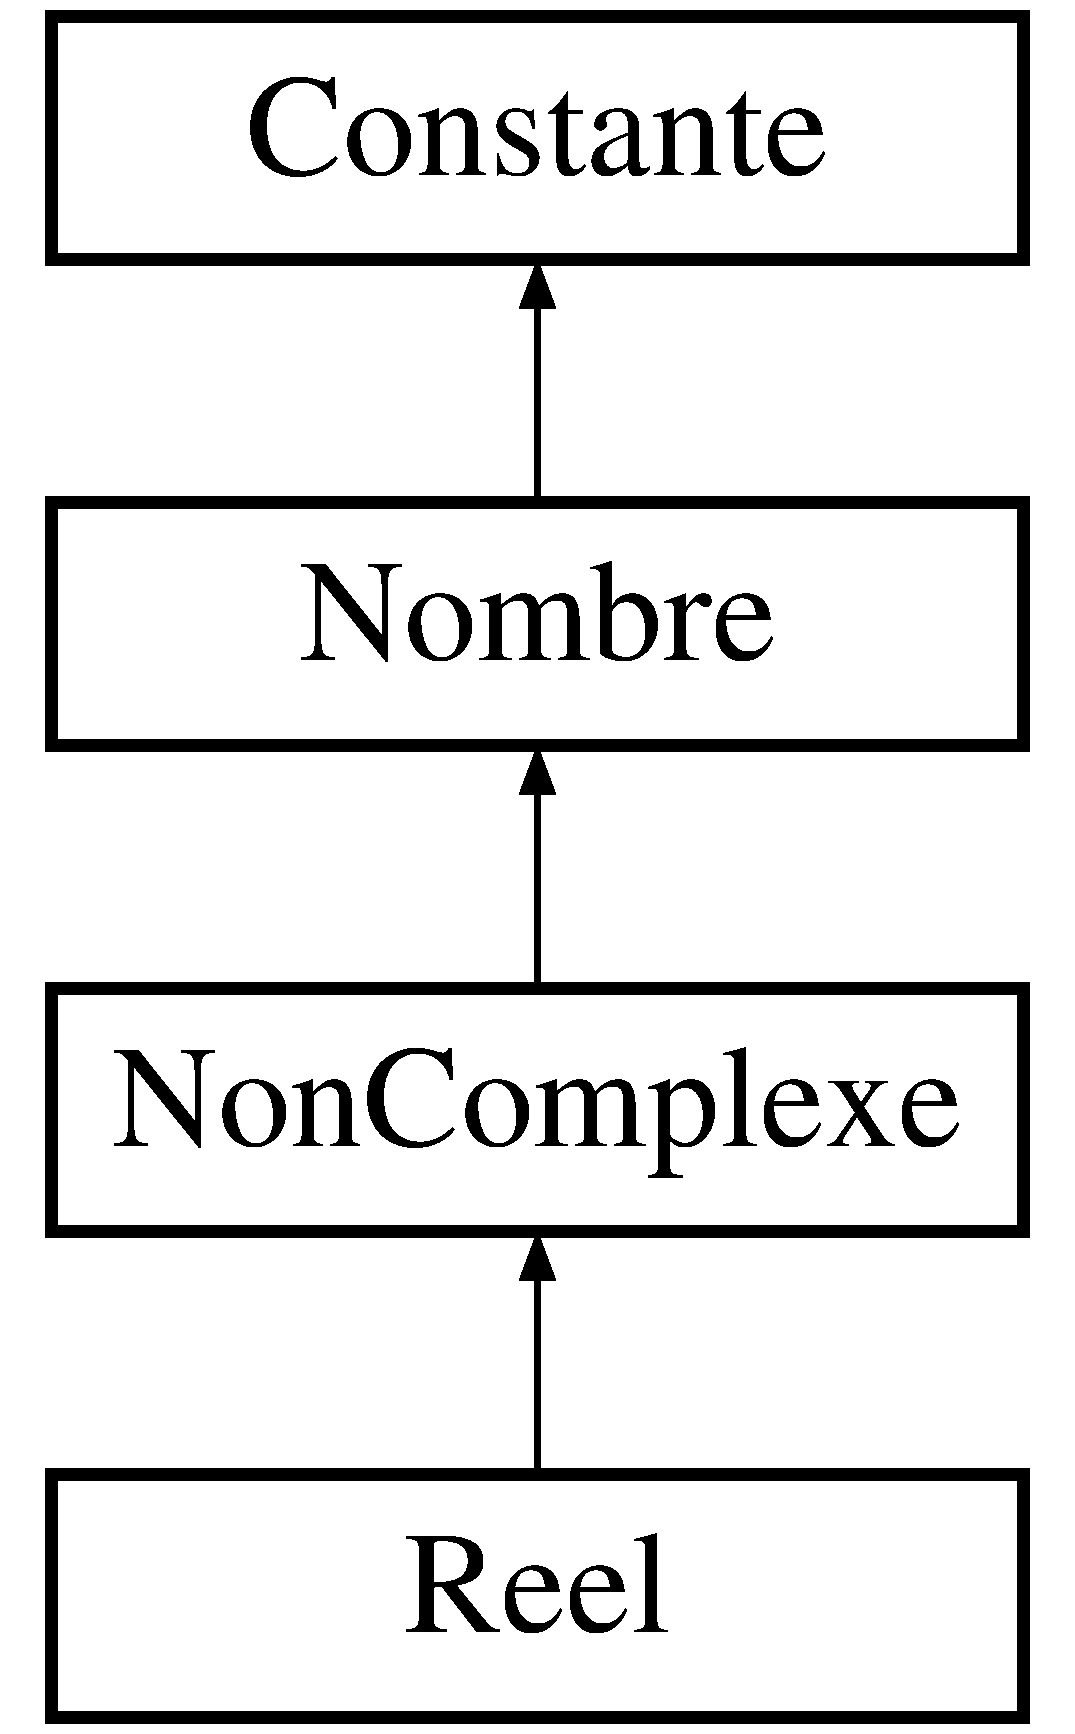
\includegraphics[height=4.000000cm]{classReel}
\end{center}
\end{figure}
\subsection*{\-Public \-Member \-Functions}
\begin{DoxyCompactItemize}
\item 
\hyperlink{classReel_a7415b4d1f436ac9499173ab43bc42fa4}{\-Reel} (float x=0)
\begin{DoxyCompactList}\small\item\em \-Crée un nombre reel. \end{DoxyCompactList}\item 
\hyperlink{classNombre}{\-Nombre} \& \hyperlink{classReel_a9bad18cd80469dfb8a16900f699abf2a}{addition} (const \hyperlink{classNombre}{\-Nombre} \&n) const 
\begin{DoxyCompactList}\small\item\em \-Calcule la somme de ce nombre reel et d'un nombre. \-Méthode virtuelle pure héritée et implémentée depuis la classe \hyperlink{classNombre}{\-Nombre}. \end{DoxyCompactList}\item 
\hyperlink{classNombre}{\-Nombre} \& \hyperlink{classReel_a5ab824ed0b29698abbe95d0edb671f97}{soustraction} (const \hyperlink{classNombre}{\-Nombre} \&n) const 
\begin{DoxyCompactList}\small\item\em \-Calcule la soustraction de ce nombre reel et d'un nombre. \-Méthode virtuelle pure héritée et implémentée depuis la classe \hyperlink{classNombre}{\-Nombre}. \end{DoxyCompactList}\item 
\hyperlink{classNombre}{\-Nombre} \& \hyperlink{classReel_a5bdfb76995bdea709a971fa2d134de46}{multiplication} (const \hyperlink{classNombre}{\-Nombre} \&n) const 
\begin{DoxyCompactList}\small\item\em \-Calcule la multiplication de ce nombre reel et d'un nombre. \-Méthode virtuelle pure héritée et implémentée depuis la classe \hyperlink{classNombre}{\-Nombre}. \end{DoxyCompactList}\item 
\hyperlink{classNombre}{\-Nombre} \& \hyperlink{classReel_a041d68cd7ee92fe30178ef1270d4628b}{division} (const \hyperlink{classNombre}{\-Nombre} \&n) const 
\begin{DoxyCompactList}\small\item\em \-Calcule la division de ce nombre reel et d'un nombre. \-Méthode virtuelle pure héritée et implémentée depuis la classe \hyperlink{classNombre}{\-Nombre}. \end{DoxyCompactList}\item 
\hyperlink{classNonComplexe}{\-Non\-Complexe} \& \hyperlink{classReel_ad9e955b349afd277bf6694aab9d928cf}{to\-Entier} () const 
\begin{DoxyCompactList}\small\item\em \-Converti le nombre reel en un nombre entier. \-Méthode virtuelle pure héritée et implémentée depuis la classe \hyperlink{classNonComplexe}{\-Non\-Complexe}. \end{DoxyCompactList}\item 
\hyperlink{classNonComplexe}{\-Non\-Complexe} \& \hyperlink{classReel_a022e6e5c75053769c7fa4f8e8bfc6fa6}{to\-Reel} () const 
\begin{DoxyCompactList}\small\item\em \-Converti le nombre reel en un nombre réel. \-Méthode virtuelle pure héritée et implémentée depuis la classe \hyperlink{classNonComplexe}{\-Non\-Complexe}. \end{DoxyCompactList}\item 
\hyperlink{classNonComplexe}{\-Non\-Complexe} \& \hyperlink{classReel_ad2c2981a8a9f140efadfef310a1c58fc}{to\-Rationnel} () const 
\begin{DoxyCompactList}\small\item\em \-Converti le nombre reel en un nombre rationnel. \-Méthode virtuelle pure héritée et implémentée depuis la classe \hyperlink{classNonComplexe}{\-Non\-Complexe}. \end{DoxyCompactList}\item 
\hyperlink{classNonComplexe}{\-Non\-Complexe} \& \hyperlink{classReel_ab8195ae116be9eca6cd69b9b03a311ba}{to\-Complexe} () const 
\begin{DoxyCompactList}\small\item\em \-Converti le nombre reel en un nombre complexe. \-Méthode virtuelle pure héritée et implémentée depuis la classe \hyperlink{classNonComplexe}{\-Non\-Complexe}. \end{DoxyCompactList}\item 
float \hyperlink{classReel_a8e0faff44febfaf4d952c6bad91b3a3f}{get\-X} () const 
\begin{DoxyCompactList}\small\item\em \-Retourne le reel de ce nombre reel. \end{DoxyCompactList}\item 
virtual \hyperlink{classReel}{\-Reel} $\ast$ \hyperlink{classReel_ab53c7d10a93c702bd7ccde897fc396df}{clone} () const 
\begin{DoxyCompactList}\small\item\em \-Crée une nouvelle instance de cette classe. \-Méthode virtuelle pure héritée et implémentée depuis la classe \hyperlink{classConstante}{\-Constante}. \end{DoxyCompactList}\item 
\-Q\-String \hyperlink{classReel_a990e8324822ba3dbc64fc7ff727411e2}{to\-String} () const 
\begin{DoxyCompactList}\small\item\em \-Retourne une chaine de caractères correspondant aux informations encapsulées par un nombre reel. \-Méthode virtuelle pure héritée et implémentée depuis la classe \hyperlink{classConstante}{\-Constante}. \end{DoxyCompactList}\end{DoxyCompactItemize}


\subsection{\-Detailed \-Description}
\-Classe permettant de créer et manipuler des constantes de type \hyperlink{classReel}{\-Reel}. \{ hérite de \hyperlink{classNonComplexe}{\-Non\-Complexe} \}. 

\subsection{\-Constructor \& \-Destructor \-Documentation}
\hypertarget{classReel_a7415b4d1f436ac9499173ab43bc42fa4}{\index{\-Reel@{\-Reel}!\-Reel@{\-Reel}}
\index{\-Reel@{\-Reel}!Reel@{\-Reel}}
\subsubsection[{\-Reel}]{\setlength{\rightskip}{0pt plus 5cm}{\bf \-Reel\-::\-Reel} (
\begin{DoxyParamCaption}
\item[{float}]{x = {\ttfamily 0}}
\end{DoxyParamCaption}
)\hspace{0.3cm}{\ttfamily  \mbox{[}inline\mbox{]}}}}\label{classReel_a7415b4d1f436ac9499173ab43bc42fa4}


\-Crée un nombre reel. 


\begin{DoxyParams}{\-Parameters}
{\em x} & \-La valeur de ce nombre reel.\\
\hline
\end{DoxyParams}
\-Crée un nombre reel de valeur donnée. 

\subsection{\-Member \-Function \-Documentation}
\hypertarget{classReel_a9bad18cd80469dfb8a16900f699abf2a}{\index{\-Reel@{\-Reel}!addition@{addition}}
\index{addition@{addition}!Reel@{\-Reel}}
\subsubsection[{addition}]{\setlength{\rightskip}{0pt plus 5cm}{\bf \-Nombre} \& {\bf \-Reel\-::addition} (
\begin{DoxyParamCaption}
\item[{const {\bf \-Nombre} \&}]{n}
\end{DoxyParamCaption}
) const\hspace{0.3cm}{\ttfamily  \mbox{[}virtual\mbox{]}}}}\label{classReel_a9bad18cd80469dfb8a16900f699abf2a}


\-Calcule la somme de ce nombre reel et d'un nombre. \-Méthode virtuelle pure héritée et implémentée depuis la classe \hyperlink{classNombre}{\-Nombre}. 


\begin{DoxyParams}{\-Parameters}
{\em n} & \-Un nombre. \\
\hline
\end{DoxyParams}
\begin{DoxyReturn}{\-Returns}
\-La somme de ce nombre reel et d'un nombre.
\end{DoxyReturn}
\-Calcule la somme de ce nombre reel et d'un nombre. 

\-Implements \hyperlink{classNonComplexe_a1ed6f047d5c576f03616535e3e92ab39}{\-Non\-Complexe}.

\hypertarget{classReel_ab53c7d10a93c702bd7ccde897fc396df}{\index{\-Reel@{\-Reel}!clone@{clone}}
\index{clone@{clone}!Reel@{\-Reel}}
\subsubsection[{clone}]{\setlength{\rightskip}{0pt plus 5cm}{\bf \-Reel} $\ast$ {\bf \-Reel\-::clone} (
\begin{DoxyParamCaption}
{}
\end{DoxyParamCaption}
) const\hspace{0.3cm}{\ttfamily  \mbox{[}inline, virtual\mbox{]}}}}\label{classReel_ab53c7d10a93c702bd7ccde897fc396df}


\-Crée une nouvelle instance de cette classe. \-Méthode virtuelle pure héritée et implémentée depuis la classe \hyperlink{classConstante}{\-Constante}. 

\begin{DoxyReturn}{\-Returns}
\-La nouvelle instance de cette classe.
\end{DoxyReturn}
\-Crée une nouvelle instance de cette classe. 

\-Implements \hyperlink{classNonComplexe_a7f1a3881b59680f3d3a7809c75ab2138}{\-Non\-Complexe}.

\hypertarget{classReel_a041d68cd7ee92fe30178ef1270d4628b}{\index{\-Reel@{\-Reel}!division@{division}}
\index{division@{division}!Reel@{\-Reel}}
\subsubsection[{division}]{\setlength{\rightskip}{0pt plus 5cm}{\bf \-Nombre} \& {\bf \-Reel\-::division} (
\begin{DoxyParamCaption}
\item[{const {\bf \-Nombre} \&}]{n}
\end{DoxyParamCaption}
) const\hspace{0.3cm}{\ttfamily  \mbox{[}virtual\mbox{]}}}}\label{classReel_a041d68cd7ee92fe30178ef1270d4628b}


\-Calcule la division de ce nombre reel et d'un nombre. \-Méthode virtuelle pure héritée et implémentée depuis la classe \hyperlink{classNombre}{\-Nombre}. 


\begin{DoxyParams}{\-Parameters}
{\em n} & \-Un nombre. \\
\hline
\end{DoxyParams}
\begin{DoxyReturn}{\-Returns}
\-La division de ce nombre reel et d'un nombre.
\end{DoxyReturn}
\-Calcule la division de ce nombre reel et d'un nombre. 

\-Implements \hyperlink{classNonComplexe_a1af698f4c7d50e69f2c7dfa3e7998cdd}{\-Non\-Complexe}.

\hypertarget{classReel_a8e0faff44febfaf4d952c6bad91b3a3f}{\index{\-Reel@{\-Reel}!get\-X@{get\-X}}
\index{get\-X@{get\-X}!Reel@{\-Reel}}
\subsubsection[{get\-X}]{\setlength{\rightskip}{0pt plus 5cm}float {\bf \-Reel\-::get\-X} (
\begin{DoxyParamCaption}
{}
\end{DoxyParamCaption}
) const\hspace{0.3cm}{\ttfamily  \mbox{[}inline\mbox{]}}}}\label{classReel_a8e0faff44febfaf4d952c6bad91b3a3f}


\-Retourne le reel de ce nombre reel. 

\begin{DoxyReturn}{\-Returns}
\-Un reel.
\end{DoxyReturn}
\-Retourne le reel de ce nombre reel. \hypertarget{classReel_a5bdfb76995bdea709a971fa2d134de46}{\index{\-Reel@{\-Reel}!multiplication@{multiplication}}
\index{multiplication@{multiplication}!Reel@{\-Reel}}
\subsubsection[{multiplication}]{\setlength{\rightskip}{0pt plus 5cm}{\bf \-Nombre} \& {\bf \-Reel\-::multiplication} (
\begin{DoxyParamCaption}
\item[{const {\bf \-Nombre} \&}]{n}
\end{DoxyParamCaption}
) const\hspace{0.3cm}{\ttfamily  \mbox{[}virtual\mbox{]}}}}\label{classReel_a5bdfb76995bdea709a971fa2d134de46}


\-Calcule la multiplication de ce nombre reel et d'un nombre. \-Méthode virtuelle pure héritée et implémentée depuis la classe \hyperlink{classNombre}{\-Nombre}. 


\begin{DoxyParams}{\-Parameters}
{\em n} & \-Un nombre. \\
\hline
\end{DoxyParams}
\begin{DoxyReturn}{\-Returns}
\-La multiplication de ce nombre reel et d'un nombre.
\end{DoxyReturn}
\-Calcule la multiplication de ce nombre reel et d'un nombre. 

\-Implements \hyperlink{classNonComplexe_a7343c4742a895813a4b031fb67170dc8}{\-Non\-Complexe}.

\hypertarget{classReel_a5ab824ed0b29698abbe95d0edb671f97}{\index{\-Reel@{\-Reel}!soustraction@{soustraction}}
\index{soustraction@{soustraction}!Reel@{\-Reel}}
\subsubsection[{soustraction}]{\setlength{\rightskip}{0pt plus 5cm}{\bf \-Nombre} \& {\bf \-Reel\-::soustraction} (
\begin{DoxyParamCaption}
\item[{const {\bf \-Nombre} \&}]{n}
\end{DoxyParamCaption}
) const\hspace{0.3cm}{\ttfamily  \mbox{[}virtual\mbox{]}}}}\label{classReel_a5ab824ed0b29698abbe95d0edb671f97}


\-Calcule la soustraction de ce nombre reel et d'un nombre. \-Méthode virtuelle pure héritée et implémentée depuis la classe \hyperlink{classNombre}{\-Nombre}. 


\begin{DoxyParams}{\-Parameters}
{\em n} & \-Un nombre. \\
\hline
\end{DoxyParams}
\begin{DoxyReturn}{\-Returns}
\-La soustraction de ce nombre reel et d'un nombre.
\end{DoxyReturn}
\-Calcule la soustraction de ce nombre reel et d'un nombre. 

\-Implements \hyperlink{classNonComplexe_ac7e41f7e2f5422687985a5fe501e243f}{\-Non\-Complexe}.

\hypertarget{classReel_ab8195ae116be9eca6cd69b9b03a311ba}{\index{\-Reel@{\-Reel}!to\-Complexe@{to\-Complexe}}
\index{to\-Complexe@{to\-Complexe}!Reel@{\-Reel}}
\subsubsection[{to\-Complexe}]{\setlength{\rightskip}{0pt plus 5cm}{\bf \-Non\-Complexe} \& {\bf \-Reel\-::to\-Complexe} (
\begin{DoxyParamCaption}
{}
\end{DoxyParamCaption}
) const\hspace{0.3cm}{\ttfamily  \mbox{[}virtual\mbox{]}}}}\label{classReel_ab8195ae116be9eca6cd69b9b03a311ba}


\-Converti le nombre reel en un nombre complexe. \-Méthode virtuelle pure héritée et implémentée depuis la classe \hyperlink{classNonComplexe}{\-Non\-Complexe}. 

\begin{DoxyReturn}{\-Returns}
\-Une référence vers un nombre non complexe emmagasinant en réalité un nombre complexe.
\end{DoxyReturn}
\-Converti le nombre reel en un nombre complexe. 

\-Implements \hyperlink{classNonComplexe_ad29a8407072d909cd204945d5cd5bc17}{\-Non\-Complexe}.

\hypertarget{classReel_ad9e955b349afd277bf6694aab9d928cf}{\index{\-Reel@{\-Reel}!to\-Entier@{to\-Entier}}
\index{to\-Entier@{to\-Entier}!Reel@{\-Reel}}
\subsubsection[{to\-Entier}]{\setlength{\rightskip}{0pt plus 5cm}{\bf \-Non\-Complexe} \& {\bf \-Reel\-::to\-Entier} (
\begin{DoxyParamCaption}
{}
\end{DoxyParamCaption}
) const\hspace{0.3cm}{\ttfamily  \mbox{[}virtual\mbox{]}}}}\label{classReel_ad9e955b349afd277bf6694aab9d928cf}


\-Converti le nombre reel en un nombre entier. \-Méthode virtuelle pure héritée et implémentée depuis la classe \hyperlink{classNonComplexe}{\-Non\-Complexe}. 

\begin{DoxyReturn}{\-Returns}
\-Une référence vers un nombre non complexe emmagasinant en réalité un nombre entier.
\end{DoxyReturn}
\-Converti le nombre reel en un nombre entier. 

\-Implements \hyperlink{classNonComplexe_af5751554285a6bf0bb1433a059bbfcdd}{\-Non\-Complexe}.

\hypertarget{classReel_ad2c2981a8a9f140efadfef310a1c58fc}{\index{\-Reel@{\-Reel}!to\-Rationnel@{to\-Rationnel}}
\index{to\-Rationnel@{to\-Rationnel}!Reel@{\-Reel}}
\subsubsection[{to\-Rationnel}]{\setlength{\rightskip}{0pt plus 5cm}{\bf \-Non\-Complexe} \& {\bf \-Reel\-::to\-Rationnel} (
\begin{DoxyParamCaption}
{}
\end{DoxyParamCaption}
) const\hspace{0.3cm}{\ttfamily  \mbox{[}virtual\mbox{]}}}}\label{classReel_ad2c2981a8a9f140efadfef310a1c58fc}


\-Converti le nombre reel en un nombre rationnel. \-Méthode virtuelle pure héritée et implémentée depuis la classe \hyperlink{classNonComplexe}{\-Non\-Complexe}. 

\begin{DoxyReturn}{\-Returns}
\-Une référence vers un nombre non complexe emmagasinant en réalité un nombre rationnel.
\end{DoxyReturn}
\-Converti le nombre reel en un nombre rationnel. 

\-Implements \hyperlink{classNonComplexe_a5c416e7c9d4c011c67b69b112cc30cc1}{\-Non\-Complexe}.

\hypertarget{classReel_a022e6e5c75053769c7fa4f8e8bfc6fa6}{\index{\-Reel@{\-Reel}!to\-Reel@{to\-Reel}}
\index{to\-Reel@{to\-Reel}!Reel@{\-Reel}}
\subsubsection[{to\-Reel}]{\setlength{\rightskip}{0pt plus 5cm}{\bf \-Non\-Complexe} \& {\bf \-Reel\-::to\-Reel} (
\begin{DoxyParamCaption}
{}
\end{DoxyParamCaption}
) const\hspace{0.3cm}{\ttfamily  \mbox{[}virtual\mbox{]}}}}\label{classReel_a022e6e5c75053769c7fa4f8e8bfc6fa6}


\-Converti le nombre reel en un nombre réel. \-Méthode virtuelle pure héritée et implémentée depuis la classe \hyperlink{classNonComplexe}{\-Non\-Complexe}. 

\begin{DoxyReturn}{\-Returns}
\-Une référence vers un nombre non complexe emmagasinant en réalité un nombre réel.
\end{DoxyReturn}
\-Converti le nombre reel en un nombre réel. 

\-Implements \hyperlink{classNonComplexe_a0bd70b66aeb18213beb9d777287540de}{\-Non\-Complexe}.

\hypertarget{classReel_a990e8324822ba3dbc64fc7ff727411e2}{\index{\-Reel@{\-Reel}!to\-String@{to\-String}}
\index{to\-String@{to\-String}!Reel@{\-Reel}}
\subsubsection[{to\-String}]{\setlength{\rightskip}{0pt plus 5cm}\-Q\-String {\bf \-Reel\-::to\-String} (
\begin{DoxyParamCaption}
{}
\end{DoxyParamCaption}
) const\hspace{0.3cm}{\ttfamily  \mbox{[}inline, virtual\mbox{]}}}}\label{classReel_a990e8324822ba3dbc64fc7ff727411e2}


\-Retourne une chaine de caractères correspondant aux informations encapsulées par un nombre reel. \-Méthode virtuelle pure héritée et implémentée depuis la classe \hyperlink{classConstante}{\-Constante}. 

\begin{DoxyReturn}{\-Returns}
\-Une chaine de caractères correspondant aux informations encapsulées par un nombre reel.
\end{DoxyReturn}
\-Retourne une chaine de caractères correspondant aux informations encapsulées par un nombre reel. 

\-Implements \hyperlink{classNonComplexe_abae1947a8f9f582f94d5e791ce4624d6}{\-Non\-Complexe}.



\-The documentation for this class was generated from the following files\-:\begin{DoxyCompactItemize}
\item 
\hyperlink{Reel_8h}{\-Reel.\-h}\item 
\-Reel.\-cpp\end{DoxyCompactItemize}

\chapter{\-File \-Documentation}
\hypertarget{BackUpPiles_8h}{\section{\-Back\-Up\-Piles.\-h \-File \-Reference}
\label{BackUpPiles_8h}\index{\-Back\-Up\-Piles.\-h@{\-Back\-Up\-Piles.\-h}}
}


\-Fichier header de la classe \hyperlink{classBackUpPiles}{\-Back\-Up\-Piles}.  


{\ttfamily \#include \char`\"{}\-Pile.\-h\char`\"{}}\*
{\ttfamily \#include $<$\-Q\-Message\-Box$>$}\*
\subsection*{\-Classes}
\begin{DoxyCompactItemize}
\item 
class \hyperlink{classBackUpPiles}{\-Back\-Up\-Piles}
\begin{DoxyCompactList}\small\item\em \-Classe permettant de garder en mémoire une liste des piles (pointeurs vers des objets de type \-Memento) ce qui permet donc de réaliser le \-Undo et le \-Redo de la pile. \end{DoxyCompactList}\end{DoxyCompactItemize}


\subsection{\-Detailed \-Description}
\-Fichier header de la classe \hyperlink{classBackUpPiles}{\-Back\-Up\-Piles}. \begin{DoxyAuthor}{\-Author}
\-Tudor \-Luchiancenco \& \-Kévin \-Njo \-Ewele 
\end{DoxyAuthor}

\hypertarget{Calculatrice_8h}{\section{\-Calculatrice.\-h \-File \-Reference}
\label{Calculatrice_8h}\index{\-Calculatrice.\-h@{\-Calculatrice.\-h}}
}


\-Fichier header de la classe \hyperlink{classCalculatrice}{\-Calculatrice}.  


{\ttfamily \#include $<$\-Q\-String$>$}\*
{\ttfamily \#include $<$\-Q\-Reg\-Exp$>$}\*
{\ttfamily \#include \char`\"{}\-Entier.\-h\char`\"{}}\*
{\ttfamily \#include \char`\"{}\-Reel.\-h\char`\"{}}\*
{\ttfamily \#include \char`\"{}\-Rationnel.\-h\char`\"{}}\*
{\ttfamily \#include \char`\"{}\-Complexe.\-h\char`\"{}}\*
\subsection*{\-Classes}
\begin{DoxyCompactItemize}
\item 
class \hyperlink{classCalculatrice}{\-Calculatrice}
\begin{DoxyCompactList}\small\item\em \-Classe permettant de créer les différentes types de constantes et de traiter les opérations. \end{DoxyCompactList}\end{DoxyCompactItemize}
\subsection*{\-Enumerations}
\begin{DoxyCompactItemize}
\item 
enum {\bfseries enum\-Type} \{ \*
{\bfseries \-E\-N\-T\-I\-E\-R}, 
{\bfseries \-R\-E\-E\-L}, 
{\bfseries \-R\-A\-T\-I\-O\-N\-N\-E\-L}, 
{\bfseries \-C\-O\-M\-P\-L\-E\-X\-E}, 
\*
{\bfseries \-E\-X\-P\-R\-E\-S\-S\-I\-O\-N}, 
{\bfseries \-O\-P\-E\-R\-A\-T\-E\-U\-R}
 \}
\end{DoxyCompactItemize}


\subsection{\-Detailed \-Description}
\-Fichier header de la classe \hyperlink{classCalculatrice}{\-Calculatrice}. \begin{DoxyAuthor}{\-Author}
\-Tudor \-Luchiancenco \& \-Kévin \-Njo \-Ewele 
\end{DoxyAuthor}

\hypertarget{CalculatriceException_8h}{\section{\-Calculatrice\-Exception.\-h \-File \-Reference}
\label{CalculatriceException_8h}\index{\-Calculatrice\-Exception.\-h@{\-Calculatrice\-Exception.\-h}}
}


\-Fichier header de la classe \hyperlink{classCalculatriceException}{\-Calculatrice\-Exception}.  


{\ttfamily \#include $<$\-Q\-String$>$}\*
{\ttfamily \#include $<$stdexcept$>$}\*
\subsection*{\-Classes}
\begin{DoxyCompactItemize}
\item 
class \hyperlink{classCalculatriceException}{\-Calculatrice\-Exception}
\begin{DoxyCompactList}\small\item\em \-Classe permettant de gérer les exceptions (problèmes d'éxécution). \{ hérite de std\-::exception \}. \end{DoxyCompactList}\end{DoxyCompactItemize}


\subsection{\-Detailed \-Description}
\-Fichier header de la classe \hyperlink{classCalculatriceException}{\-Calculatrice\-Exception}. \begin{DoxyAuthor}{\-Author}
\-Tudor \-Luchiancenco \& \-Kévin \-Njo \-Ewele 
\end{DoxyAuthor}

\hypertarget{Complexe_8h}{\section{\-Complexe.\-h \-File \-Reference}
\label{Complexe_8h}\index{\-Complexe.\-h@{\-Complexe.\-h}}
}


\-Fichier header de la classe \hyperlink{classComplexe}{\-Complexe}.  


{\ttfamily \#include \char`\"{}\-Non\-Complexe.\-h\char`\"{}}\*
{\ttfamily \#include \char`\"{}\-Nombre.\-h\char`\"{}}\*
\subsection*{\-Classes}
\begin{DoxyCompactItemize}
\item 
class \hyperlink{classComplexe}{\-Complexe}
\begin{DoxyCompactList}\small\item\em \-Classe permettant de créer et manipuler des constantes de type \hyperlink{classComplexe}{\-Complexe}. \{ hérite de \hyperlink{classNombre}{\-Nombre} \}. \end{DoxyCompactList}\end{DoxyCompactItemize}


\subsection{\-Detailed \-Description}
\-Fichier header de la classe \hyperlink{classComplexe}{\-Complexe}. \begin{DoxyAuthor}{\-Author}
\-Tudor \-Luchiancenco \& \-Kévin \-Njo \-Ewele 
\end{DoxyAuthor}

\hypertarget{Constante_8h}{\section{\-Constante.\-h \-File \-Reference}
\label{Constante_8h}\index{\-Constante.\-h@{\-Constante.\-h}}
}


\-Fichier header de la classe \hyperlink{classConstante}{\-Constante}.  


{\ttfamily \#include $<$\-Q\-Text\-Stream$>$}\*
{\ttfamily \#include \char`\"{}\-Calculatrice\-Exception.\-h\char`\"{}}\*
\subsection*{\-Classes}
\begin{DoxyCompactItemize}
\item 
class \hyperlink{classConstante}{\-Constante}
\begin{DoxyCompactList}\small\item\em \-Classe abstraite étant utilisée comme interface pour les classes qui en héritent. \end{DoxyCompactList}\end{DoxyCompactItemize}
\subsection*{\-Functions}
\begin{DoxyCompactItemize}
\item 
\hypertarget{Constante_8h_ab55c8a6e65e13388d5ce68d9af01ce89}{\-Q\-Text\-Stream \& {\bfseries operator$<$$<$} (\-Q\-Text\-Stream \&f, const \hyperlink{classConstante}{\-Constante} \&c)}\label{Constante_8h_ab55c8a6e65e13388d5ce68d9af01ce89}

\end{DoxyCompactItemize}


\subsection{\-Detailed \-Description}
\-Fichier header de la classe \hyperlink{classConstante}{\-Constante}. \begin{DoxyAuthor}{\-Author}
\-Tudor \-Luchiancenco \& \-Kévin \-Njo \-Ewele 
\end{DoxyAuthor}

\hypertarget{dialog_8h}{\section{dialog.\-h \-File \-Reference}
\label{dialog_8h}\index{dialog.\-h@{dialog.\-h}}
}


\-Fichier header de la classe \hyperlink{classDialog}{\-Dialog}.  


{\ttfamily \#include $<$\-Q\-Dialog$>$}\*
\subsection*{\-Classes}
\begin{DoxyCompactItemize}
\item 
class \hyperlink{classDialog}{\-Dialog}
\end{DoxyCompactItemize}


\subsection{\-Detailed \-Description}
\-Fichier header de la classe \hyperlink{classDialog}{\-Dialog}. \begin{DoxyAuthor}{\-Author}
\-Tudor \-Luchiancenco \& \-Kévin \-Njo \-Ewele 
\end{DoxyAuthor}

\hypertarget{Entier_8h}{\section{\-Entier.\-h \-File \-Reference}
\label{Entier_8h}\index{\-Entier.\-h@{\-Entier.\-h}}
}


\-Fichier header de la classe \hyperlink{classEntier}{\-Entier}.  


{\ttfamily \#include \char`\"{}\-Non\-Complexe.\-h\char`\"{}}\*
{\ttfamily \#include \char`\"{}\-Rationnel.\-h\char`\"{}}\*
{\ttfamily \#include \char`\"{}\-Reel.\-h\char`\"{}}\*
{\ttfamily \#include \char`\"{}\-Complexe.\-h\char`\"{}}\*
\subsection*{\-Classes}
\begin{DoxyCompactItemize}
\item 
class \hyperlink{classEntier}{\-Entier}
\begin{DoxyCompactList}\small\item\em \-Classe permettant de créer et manipuler des constantes de type \hyperlink{classEntier}{\-Entier}. \{ hérite de \hyperlink{classNonComplexe}{\-Non\-Complexe} \}. \end{DoxyCompactList}\end{DoxyCompactItemize}
\subsection*{\-Functions}
\begin{DoxyCompactItemize}
\item 
\hypertarget{Entier_8h_acf8e9299cf32eef32d8461cd7c1cb8c4}{int {\bfseries factorielle} (int n)}\label{Entier_8h_acf8e9299cf32eef32d8461cd7c1cb8c4}

\end{DoxyCompactItemize}


\subsection{\-Detailed \-Description}
\-Fichier header de la classe \hyperlink{classEntier}{\-Entier}. \begin{DoxyAuthor}{\-Author}
\-Tudor \-Luchiancenco \& \-Kévin \-Njo \-Ewele 
\end{DoxyAuthor}

\hypertarget{Expression_8h}{\section{\-Expression.\-h \-File \-Reference}
\label{Expression_8h}\index{\-Expression.\-h@{\-Expression.\-h}}
}


\-Fichier header de la classe \hyperlink{classExpression}{\-Expression}.  


{\ttfamily \#include $<$\-Q\-Text\-Stream$>$}\*
{\ttfamily \#include $<$\-Q\-String$>$}\*
{\ttfamily \#include \char`\"{}\-Constante.\-h\char`\"{}}\*
\subsection*{\-Classes}
\begin{DoxyCompactItemize}
\item 
class \hyperlink{classExpression}{\-Expression}
\begin{DoxyCompactList}\small\item\em \-Classe permettant de créer et manipuler des constantes de type \hyperlink{classExpression}{\-Expression}. \{ hérite de \hyperlink{classConstante}{\-Constante} \}. \end{DoxyCompactList}\end{DoxyCompactItemize}


\subsection{\-Detailed \-Description}
\-Fichier header de la classe \hyperlink{classExpression}{\-Expression}. \begin{DoxyAuthor}{\-Author}
\-Tudor \-Luchiancenco \& \-Kévin \-Njo \-Ewele 
\end{DoxyAuthor}

\hypertarget{LogMessage_8h}{\section{\-Log\-Message.\-h \-File \-Reference}
\label{LogMessage_8h}\index{\-Log\-Message.\-h@{\-Log\-Message.\-h}}
}


\-Fichier header de la classe \hyperlink{classLogMessage}{\-Log\-Message}.  


{\ttfamily \#include $<$\-Q\-String$>$}\*
{\ttfamily \#include $<$ctime$>$}\*
\subsection*{\-Classes}
\begin{DoxyCompactItemize}
\item 
class \hyperlink{classLogMessage}{\-Log\-Message}
\begin{DoxyCompactList}\small\item\em \-Classe permettant de créer et manipuler des messages de log. \end{DoxyCompactList}\end{DoxyCompactItemize}
\subsection*{\-Enumerations}
\begin{DoxyCompactItemize}
\item 
enum \hyperlink{LogMessage_8h_a1d3861c8dbb6437102a5f0d835982b80}{enum\-Importance} \{ {\bfseries \-F\-A\-I\-B\-L\-E}, 
{\bfseries \-M\-O\-Y\-E\-N\-N\-E}, 
{\bfseries \-E\-L\-E\-V\-E\-E}
 \}
\end{DoxyCompactItemize}


\subsection{\-Detailed \-Description}
\-Fichier header de la classe \hyperlink{classLogMessage}{\-Log\-Message}. \begin{DoxyAuthor}{\-Author}
\-Tudor \-Luchiancenco \& \-Kévin \-Njo \-Ewele 
\end{DoxyAuthor}


\subsection{\-Enumeration \-Type \-Documentation}
\hypertarget{LogMessage_8h_a1d3861c8dbb6437102a5f0d835982b80}{\index{\-Log\-Message.\-h@{\-Log\-Message.\-h}!enum\-Importance@{enum\-Importance}}
\index{enum\-Importance@{enum\-Importance}!LogMessage.h@{\-Log\-Message.\-h}}
\subsubsection[{enum\-Importance}]{\setlength{\rightskip}{0pt plus 5cm}enum {\bf enum\-Importance}}}\label{LogMessage_8h_a1d3861c8dbb6437102a5f0d835982b80}
$<$ \-Les degrés d'importance d'un message de log. 
\hypertarget{LogSystem_8h}{\section{\-Log\-System.\-h \-File \-Reference}
\label{LogSystem_8h}\index{\-Log\-System.\-h@{\-Log\-System.\-h}}
}


\-Fichier header de la classe \hyperlink{classLogSystem}{\-Log\-System}.  


{\ttfamily \#include \char`\"{}\-Log\-Message.\-h\char`\"{}}\*
{\ttfamily \#include $<$\-Q\-String$>$}\*
\subsection*{\-Classes}
\begin{DoxyCompactItemize}
\item 
class \hyperlink{classLogSystem}{\-Log\-System}
\begin{DoxyCompactList}\small\item\em \-Classe permettant d'écrire des messages de log dans un fichier spécifique. \end{DoxyCompactList}\end{DoxyCompactItemize}


\subsection{\-Detailed \-Description}
\-Fichier header de la classe \hyperlink{classLogSystem}{\-Log\-System}. \begin{DoxyAuthor}{\-Author}
\-Tudor \-Luchiancenco \& \-Kévin \-Njo \-Ewele 
\end{DoxyAuthor}

\hypertarget{mainwindow_8h}{\section{mainwindow.\-h \-File \-Reference}
\label{mainwindow_8h}\index{mainwindow.\-h@{mainwindow.\-h}}
}


\-Fichier header de la classe \hyperlink{classMainWindow}{\-Main\-Window}.  


{\ttfamily \#include $<$\-Q\-Main\-Window$>$}\*
{\ttfamily \#include $<$iterator$>$}\*
{\ttfamily \#include $<$\-Q\-String$>$}\*
{\ttfamily \#include $<$\-Q\-List$>$}\*
{\ttfamily \#include $<$\-Q\-Text\-Stream$>$}\*
{\ttfamily \#include $<$\-Q\-Char$>$}\*
{\ttfamily \#include \char`\"{}\-Calculatrice.\-h\char`\"{}}\*
{\ttfamily \#include \char`\"{}dialog.\-h\char`\"{}}\*
\subsection*{\-Classes}
\begin{DoxyCompactItemize}
\item 
class \hyperlink{classMainWindow}{\-Main\-Window}
\end{DoxyCompactItemize}
\subsection*{\-Functions}
\begin{DoxyCompactItemize}
\item 
\hypertarget{mainwindow_8h_addbc789542445d2e1b8cf01582c975e3}{int {\bfseries rand\-Int} ()}\label{mainwindow_8h_addbc789542445d2e1b8cf01582c975e3}

\end{DoxyCompactItemize}


\subsection{\-Detailed \-Description}
\-Fichier header de la classe \hyperlink{classMainWindow}{\-Main\-Window}. \begin{DoxyAuthor}{\-Author}
\-Tudor \-Luchiancenco \& \-Kévin \-Njo \-Ewele 
\end{DoxyAuthor}

\hypertarget{Nombre_8h}{\section{\-Nombre.\-h \-File \-Reference}
\label{Nombre_8h}\index{\-Nombre.\-h@{\-Nombre.\-h}}
}


\-Fichier header de la classe \hyperlink{classNombre}{\-Nombre}.  


{\ttfamily \#include $<$\-Q\-String$>$}\*
{\ttfamily \#include \char`\"{}\-Constante.\-h\char`\"{}}\*
\subsection*{\-Classes}
\begin{DoxyCompactItemize}
\item 
class \hyperlink{classNombre}{\-Nombre}
\begin{DoxyCompactList}\small\item\em \-Classe abstraite étant utilisée comme interface pour les classes qui en héritent. \{ hérite de \hyperlink{classConstante}{\-Constante} \}. \end{DoxyCompactList}\end{DoxyCompactItemize}


\subsection{\-Detailed \-Description}
\-Fichier header de la classe \hyperlink{classNombre}{\-Nombre}. \begin{DoxyAuthor}{\-Author}
\-Tudor \-Luchiancenco \& \-Kévin \-Njo \-Ewele 
\end{DoxyAuthor}

\hypertarget{NonComplexe_8h}{\section{\-Non\-Complexe.\-h \-File \-Reference}
\label{NonComplexe_8h}\index{\-Non\-Complexe.\-h@{\-Non\-Complexe.\-h}}
}


\-Fichier header de la classe \hyperlink{classNonComplexe}{\-Non\-Complexe}.  


{\ttfamily \#include \char`\"{}\-Nombre.\-h\char`\"{}}\*
\subsection*{\-Classes}
\begin{DoxyCompactItemize}
\item 
class \hyperlink{classNonComplexe}{\-Non\-Complexe}
\begin{DoxyCompactList}\small\item\em \-Classe permettant de créer et manipuler des constantes de type \hyperlink{classNonComplexe}{\-Non\-Complexe}, fourni également une interface aux classes qui en héritent. \{ hérite de \hyperlink{classNombre}{\-Nombre} \}. \end{DoxyCompactList}\end{DoxyCompactItemize}


\subsection{\-Detailed \-Description}
\-Fichier header de la classe \hyperlink{classNonComplexe}{\-Non\-Complexe}. \begin{DoxyAuthor}{\-Author}
\-Tudor \-Luchiancenco \& \-Kévin \-Njo \-Ewele 
\end{DoxyAuthor}

\hypertarget{Operateur_8h}{\section{\-Operateur.\-h \-File \-Reference}
\label{Operateur_8h}\index{\-Operateur.\-h@{\-Operateur.\-h}}
}


\-Fichier header de la classe \hyperlink{classOperateur}{\-Operateur}.  


{\ttfamily \#include $<$\-Q\-String$>$}\*
{\ttfamily \#include \char`\"{}\-Calculatrice\-Exception.\-h\char`\"{}}\*
\subsection*{\-Classes}
\begin{DoxyCompactItemize}
\item 
class \hyperlink{classOperateur}{\-Operateur}
\begin{DoxyCompactList}\small\item\em \-Classe permettant de créer et manipuler des opérateurs. \end{DoxyCompactList}\end{DoxyCompactItemize}
\subsection*{\-Enumerations}
\begin{DoxyCompactItemize}
\item 
enum \hyperlink{Operateur_8h_a5cba6a46a0d2fa21cdb37232c23cd8f9}{enum\-Operateur} \{ \*
{\bfseries \-A\-D\-D}, 
{\bfseries \-S\-O\-U\-S}, 
{\bfseries \-M\-U\-L}, 
{\bfseries \-D\-I\-V}, 
\*
{\bfseries \-P\-O\-W}, 
{\bfseries \-M\-O\-D}, 
{\bfseries \-F\-A\-C\-T}, 
{\bfseries \-C\-O\-S}, 
\*
{\bfseries \-S\-I\-N}, 
{\bfseries \-T\-A\-N}, 
{\bfseries \-C\-O\-S\-H}, 
{\bfseries \-S\-I\-N\-H}, 
\*
{\bfseries \-T\-A\-N\-H}, 
{\bfseries \-L\-N}, 
{\bfseries \-I\-N\-V}, 
{\bfseries \-L\-O\-G}, 
\*
{\bfseries \-S\-Q\-R\-T}, 
{\bfseries \-E\-V\-A\-L}, 
{\bfseries \-S\-Q\-R}, 
{\bfseries \-C\-U\-B\-E}, 
\*
{\bfseries \-S\-I\-G\-N}, 
{\bfseries \-S\-W\-A\-P}, 
{\bfseries \-S\-U\-M}, 
{\bfseries \-M\-E\-A\-N}, 
\*
{\bfseries \-C\-L\-E\-A\-R}, 
{\bfseries \-D\-U\-P}, 
{\bfseries \-D\-R\-O\-P}
 \}
\end{DoxyCompactItemize}


\subsection{\-Detailed \-Description}
\-Fichier header de la classe \hyperlink{classOperateur}{\-Operateur}. \begin{DoxyAuthor}{\-Author}
\-Tudor \-Luchiancenco \& \-Kévin \-Njo \-Ewele 
\end{DoxyAuthor}


\subsection{\-Enumeration \-Type \-Documentation}
\hypertarget{Operateur_8h_a5cba6a46a0d2fa21cdb37232c23cd8f9}{\index{\-Operateur.\-h@{\-Operateur.\-h}!enum\-Operateur@{enum\-Operateur}}
\index{enum\-Operateur@{enum\-Operateur}!Operateur.h@{\-Operateur.\-h}}
\subsubsection[{enum\-Operateur}]{\setlength{\rightskip}{0pt plus 5cm}enum {\bf enum\-Operateur}}}\label{Operateur_8h_a5cba6a46a0d2fa21cdb37232c23cd8f9}
$<$ \-Les opérateurs valides. 
\hypertarget{Pile_8h}{\section{\-Pile.\-h \-File \-Reference}
\label{Pile_8h}\index{\-Pile.\-h@{\-Pile.\-h}}
}


\-Fichier header de la classe \hyperlink{classPile}{\-Pile}.  


{\ttfamily \#include \char`\"{}\-Q\-Stack\char`\"{}}\*
{\ttfamily \#include \char`\"{}\-Constante.\-h\char`\"{}}\*
\subsection*{\-Classes}
\begin{DoxyCompactItemize}
\item 
class \hyperlink{classPile}{\-Pile}
\begin{DoxyCompactList}\small\item\em \-Classe permettant de stocker les différentes constantes et résultats de calculs de l'utilisateur de la calculatrice. \{ hérite de \-Q\-Stack$<$\-Constante$\ast$$>$ \}. \end{DoxyCompactList}\item 
class \hyperlink{classPile_1_1Memento}{\-Pile\-::\-Memento}
\end{DoxyCompactItemize}


\subsection{\-Detailed \-Description}
\-Fichier header de la classe \hyperlink{classPile}{\-Pile}. \begin{DoxyAuthor}{\-Author}
\-Tudor \-Luchiancenco \& \-Kévin \-Njo \-Ewele 
\end{DoxyAuthor}

\hypertarget{PileAffichage_8h}{\section{\-Pile\-Affichage.\-h \-File \-Reference}
\label{PileAffichage_8h}\index{\-Pile\-Affichage.\-h@{\-Pile\-Affichage.\-h}}
}


\-Fichier header de la classe \hyperlink{classPileAffichage}{\-Pile\-Affichage}.  


{\ttfamily \#include $<$\-Q\-Stack$>$}\*
{\ttfamily \#include $<$\-Q\-String$>$}\*
\subsection*{\-Classes}
\begin{DoxyCompactItemize}
\item 
class \hyperlink{classPileAffichage}{\-Pile\-Affichage}
\begin{DoxyCompactList}\small\item\em \-Classe permettant de stocker les différentes constantes et résultats de calculs de l'utilisateur de la calculatrice, mais également les opérateurs. \{ hérite de \-Q\-Stack$<$\-Q\-String$>$ \}. \end{DoxyCompactList}\end{DoxyCompactItemize}


\subsection{\-Detailed \-Description}
\-Fichier header de la classe \hyperlink{classPileAffichage}{\-Pile\-Affichage}. \begin{DoxyAuthor}{\-Author}
\-Tudor \-Luchiancenco \& \-Kévin \-Njo \-Ewele 
\end{DoxyAuthor}

\hypertarget{Rationnel_8h}{\section{\-Rationnel.\-h \-File \-Reference}
\label{Rationnel_8h}\index{\-Rationnel.\-h@{\-Rationnel.\-h}}
}


\-Fichier header de la classe \hyperlink{classRationnel}{\-Rationnel}.  


{\ttfamily \#include \char`\"{}\-Non\-Complexe.\-h\char`\"{}}\*
{\ttfamily \#include \char`\"{}\-Entier.\-h\char`\"{}}\*
{\ttfamily \#include \char`\"{}\-Reel.\-h\char`\"{}}\*
{\ttfamily \#include \char`\"{}\-Complexe.\-h\char`\"{}}\*
\subsection*{\-Classes}
\begin{DoxyCompactItemize}
\item 
class \hyperlink{classRationnel}{\-Rationnel}
\begin{DoxyCompactList}\small\item\em \-Classe permettant de créer et manipuler des constantes de type \hyperlink{classRationnel}{\-Rationnel}. \{ hérite de \hyperlink{classNonComplexe}{\-Non\-Complexe} \}. \end{DoxyCompactList}\end{DoxyCompactItemize}
\subsection*{\-Functions}
\begin{DoxyCompactItemize}
\item 
\hypertarget{Rationnel_8h_a849af74e3699c79923a435b22f6942ba}{\hyperlink{classEntier}{\-Entier} {\bfseries pgcd} (const \hyperlink{classEntier}{\-Entier} \&a, const \hyperlink{classEntier}{\-Entier} \&b)}\label{Rationnel_8h_a849af74e3699c79923a435b22f6942ba}

\end{DoxyCompactItemize}


\subsection{\-Detailed \-Description}
\-Fichier header de la classe \hyperlink{classRationnel}{\-Rationnel}. \begin{DoxyAuthor}{\-Author}
\-Tudor \-Luchiancenco \& \-Kévin \-Njo \-Ewele 
\end{DoxyAuthor}

\hypertarget{Reel_8h}{\section{\-Reel.\-h \-File \-Reference}
\label{Reel_8h}\index{\-Reel.\-h@{\-Reel.\-h}}
}


\-Fichier header de la classe \hyperlink{classReel}{\-Reel}.  


{\ttfamily \#include \char`\"{}\-Non\-Complexe.\-h\char`\"{}}\*
{\ttfamily \#include \char`\"{}\-Entier.\-h\char`\"{}}\*
{\ttfamily \#include \char`\"{}\-Rationnel.\-h\char`\"{}}\*
{\ttfamily \#include \char`\"{}\-Complexe.\-h\char`\"{}}\*
\subsection*{\-Classes}
\begin{DoxyCompactItemize}
\item 
class \hyperlink{classReel}{\-Reel}
\begin{DoxyCompactList}\small\item\em \-Classe permettant de créer et manipuler des constantes de type \hyperlink{classReel}{\-Reel}. \{ hérite de \hyperlink{classNonComplexe}{\-Non\-Complexe} \}. \end{DoxyCompactList}\end{DoxyCompactItemize}


\subsection{\-Detailed \-Description}
\-Fichier header de la classe \hyperlink{classReel}{\-Reel}. \begin{DoxyAuthor}{\-Author}
\-Tudor \-Luchiancenco \& \-Kévin \-Njo \-Ewele 
\end{DoxyAuthor}

\printindex
\end{document}
